\section{Introduction}
The main goal of many scientific disciplines can be summarized to the following:

\begin{enumerate}
\item Formulate a set of mathematical equations to model a phenomena of interest
\item Analyze solutions to these equations in order to extract information and make predictions.
\end{enumerate}

The result of (1) is often a system of partial differential equations, thus the second becomes solving those equations.
\ \\ 
\begin{definition}[Partial Differential Equation]
    A partial differential equation (PDE) is a differential equation containing partial derivatives of the dependent variable with respect to more than one independent variable.
\end{definition}

\subsection{Classification Of PDEs}
\subsubsection{Order of PDE}
The order of a PDE is determined by the highest derivative in the equation.
\begin{align*}
\frac{\partial u}{\partial t} + {(\frac{\partial u}{\partial x})}^2 &= 0 \ \ \ \ \Longrightarrow  \text{First Order}
\\
\frac{\partial^4 u}{\partial y^4} + \frac{\partial u}{\partial x} &= c \ \ \ \ \Longrightarrow  \text{Fourth Order}
\end{align*}
Do not mistake the order of the PDE with its degree, the degree of the PDE is the highest exponent appearing in the equation.
\subsubsection{Linearity} 
A linear PDE is one that is of first degree in all of it's field variables and partial derivatives.
\begin{alignat*}{2}
&\frac{\partial u}{\partial t} + \frac{\partial u}{\partial x} = 0 &\dquad &\text{linear}
\\
&\frac{\partial^4 u}{\partial y^4} + \frac{\partial u}{\partial x} = y &\dquad &\text{linear}
\\
&\frac{\partial u}{\partial t} + {(\frac{\partial u}{\partial x})}^2 = 0 &\dquad &\text{nonlinear}
\\
&\frac{\partial^3 u}{\partial x^3} + {(\frac{\partial^2 u}{\partial y^2})}^5 = \sin(x) &\dquad &\text{nonlinear}
\end{alignat*}

A linear operator can be defined for any linear equation, taking the first equation in the previous list, the linear operator $L$ can be defined as.
\[
L = \frac{\partial u }{\partial t} + \frac{\partial u}{\partial x}
\]
And the equation can be written as.
\[
    L(u)=0    
\]

\subsubsection{Homogeneity}
Let $L$ be a linear operator. Then a linear partial differential equation can be written in the form.
\[
    L(u) = f(x_1,x_2, \dots , t)    
\]
If $f = 0$ then the equation is homogeneous, otherwise it is inhomogeneous.
\begin{align*}
\frac{\partial u}{\partial t} + \frac{\partial u}{\partial x} &= 0 \dquad \text{homogeneous}
\\
\frac{\partial^4 u}{\partial y^4} + \frac{\partial u}{\partial x} &= y \dquad \text{inhomogeneous}
\end{align*}

\newpage

\subsection{Boundary Conditions}
\
\begin{definition}[Boundary Conditions]
    Boundary conditions are constraints describes the function at the ends of it's region and they are necessary for the solution of a boundary value problem.
\end{definition}
\begin{definition}[Boundary Value Problem]
    BVP is a differential equation to be solved in a domain on whose boundary the function is known.
\end{definition}
We will be interested in one type of boundary conditions in this course which is the Dirichlet Conditions, specifies the value that the unknown function needs to take on along the boundary of the domain. For example, the Laplace equation on a circle with Dirichlet condition will be.
\[
    \nabla^2 u(x) = 0 \quad \forall x \in G    
\]
\[
    u(x) = f(x) \quad \forall x \in \Gamma    
\]
\begin{center}
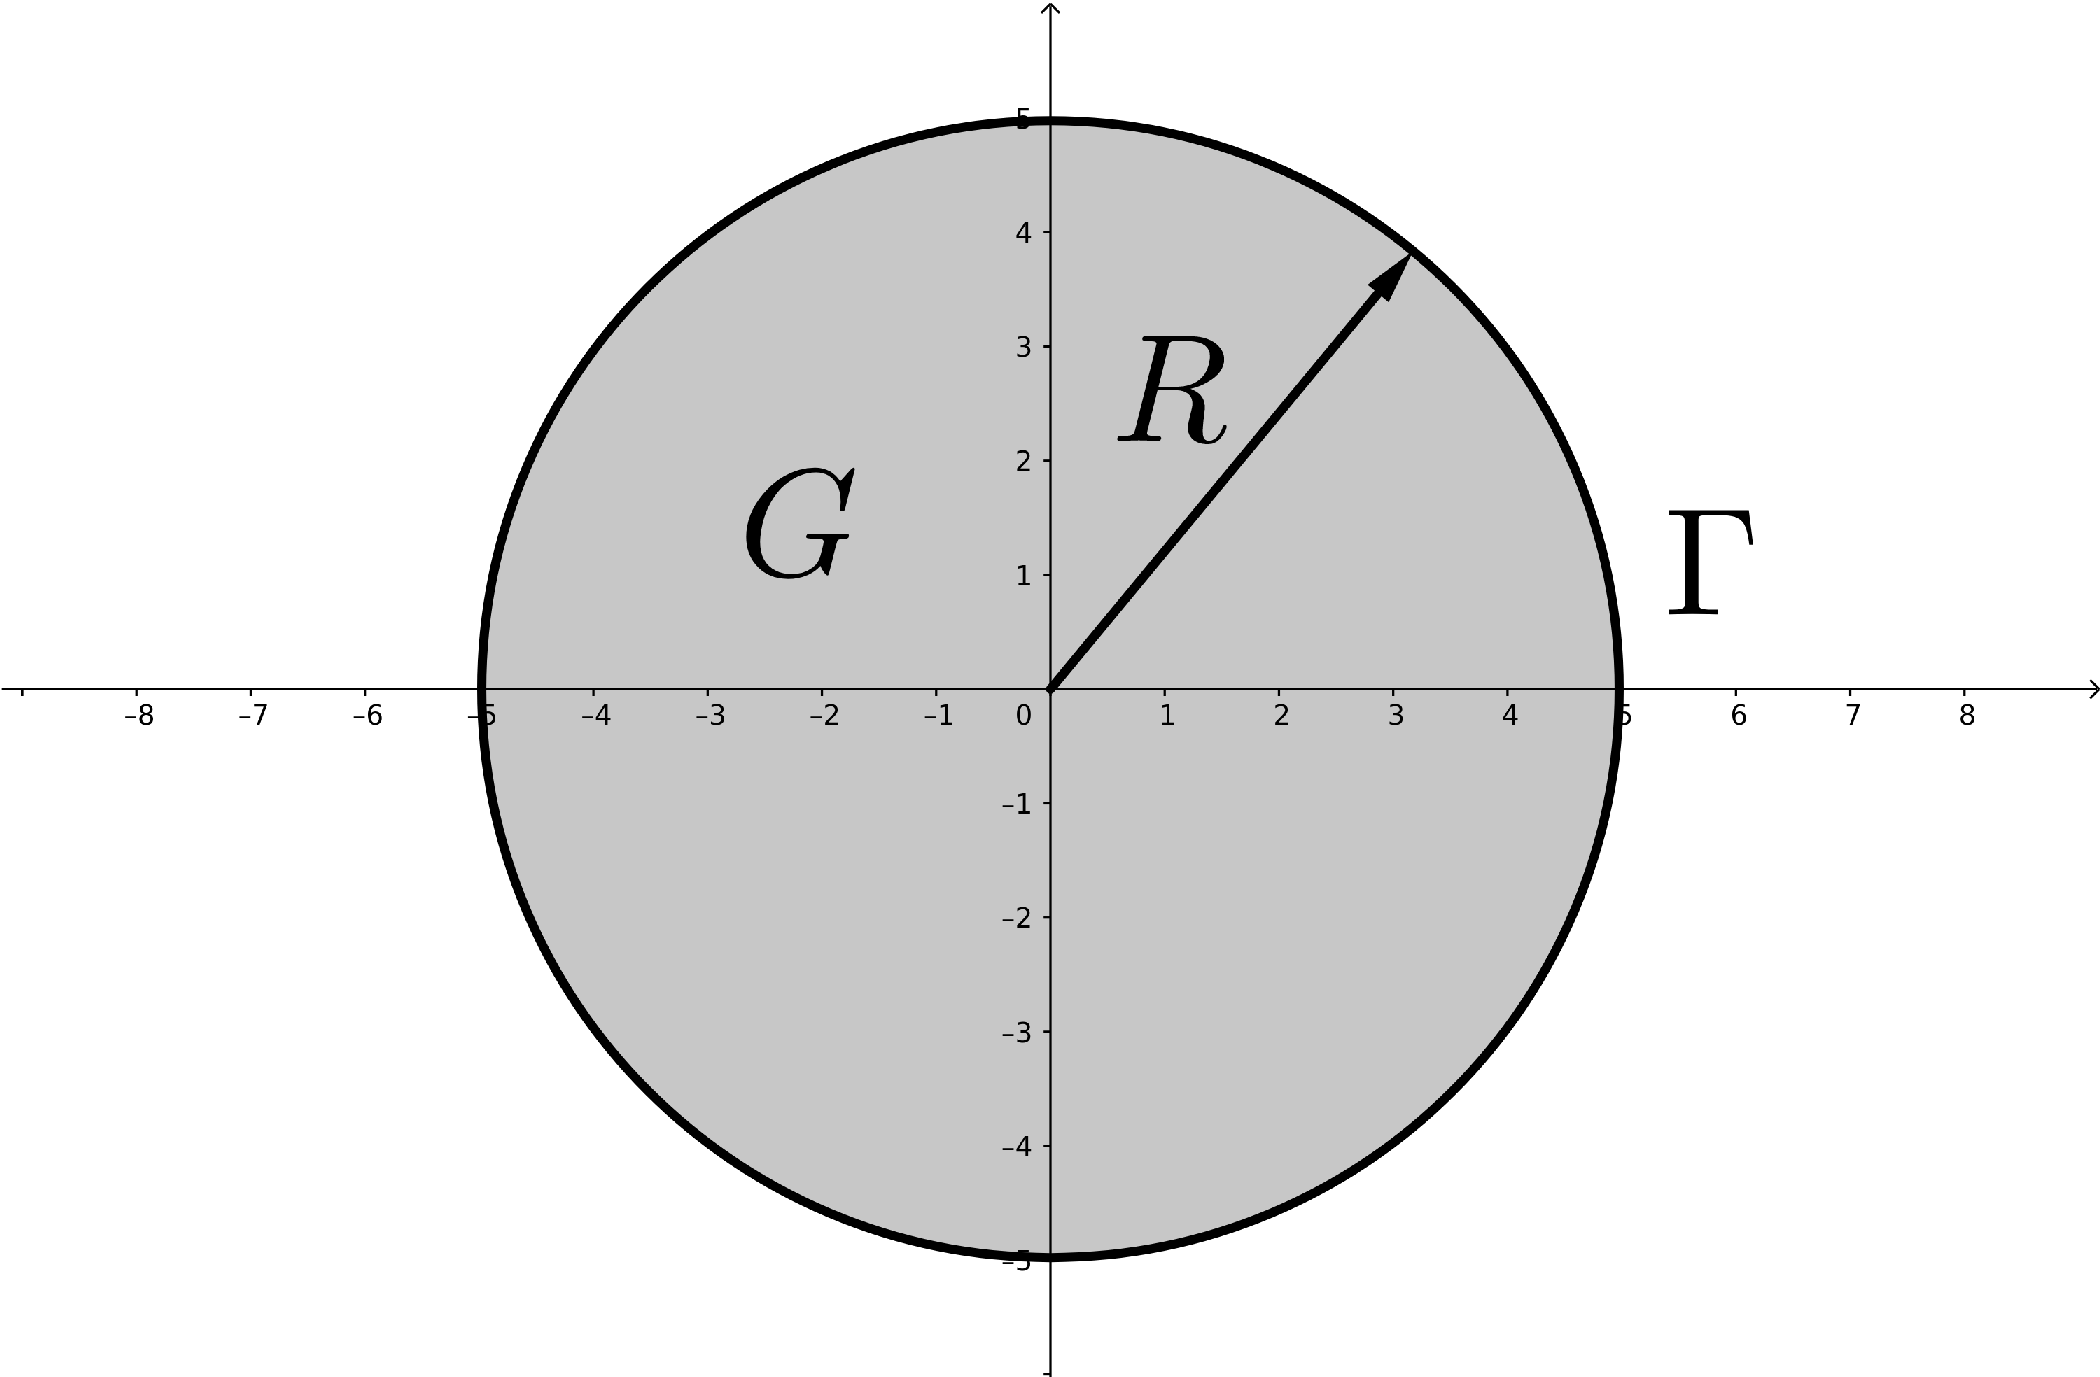
\includegraphics[scale=0.1]{laplacecircle.png} 
\end{center}
\[
    G = \left\lbrace (x,y):x^2+y^2 < R^2 \right\rbrace  \dquad \Gamma = \left\lbrace (x,y):x^2+y^2 = R^2 \right\rbrace    
\]
\begin{definition}[Dirichlet Problems]
    are problems that has only boundary conditions
\end{definition}
\subsection{Initial Condition}
\
\begin{definition}[The Initial Condition]
    is a condition that a solution must have at only on instant of time, which is the starting time as it can be found experimentally.
\end{definition}
An example is the heat equation with initial condition.
\[
    \frac{\partial u(x,t)}{\partial t}  = c^2 \frac{\partial u(x,t)}{\partial x}
\]
\[
    u(x,0) = f(x)
\]
\begin{definition}[Cauchy Problems]
    are problems that has only initial conditions
\end{definition}

\begin{figure*}[b]
    \begin{minipage}[h]{\textwidth}
        \begin{enrichment}{Dirichlet}{Dirichlet.jpg}{2.4}{.8}{.17}
            Peter Gustav Lejeune Dirichlet (1805-1859)  Born in Düren, Germany, Dirichlet's work on boundary value problems, particularly for the Poisson equation, laid the foundation for modern PDE theory. Dirichlet introduced "Dirichlet boundary conditions," enabling unique solutions and influencing various scientific and engineering disciplines. His principle for potential theory remains vital in mathematical physics, making him a prominent figure in PDE history.
        \end{enrichment}
    \end{minipage}
\end{figure*}


\newpage
\section{Canonical Form}
In this section, we shall show that coordinate transformations can be employed successfully to reduce second-order linear PDEs to some standard forms known as canonical forms. 
\\
These transformed equations can sometimes be solved rather easily.


Consider the following PDE with variable coefficients. We are aiming to transform this equation into its canonical form
\begin{equation}
A\left(x,y\right)\frac{\partial^2 u\left(x,y\right)}{\partial x^2} + 2B\left(x,y\right)\frac{\partial^2 u\left(x,y\right)}{\partial x\partial y}+C\left(x,y\right)\frac{\partial^2 u\left(x,y\right)}{\partial y^2}+F\left(x,y,u,\frac{\partial u}{\partial x},\frac{\partial u}{\partial y}\right) = 0
\end{equation}
The first three terms are called the principle terms and the last term is called the Young term
\vspace*{.2cm}
\begin{definition}[Young Term]
    are terms which does not contain second order derivatives of the function
\end{definition}
\par
We start by preforming a change of variables such that.
\[
    \xi = \xi\left(x,y\right)\quad,\quad\eta = \eta\left(x,y\right)    
\]
Taking into consideration the Jacobian of the transformation
\[
    J =\begin{vmatrix} \frac{\partial\xi}{\partial x}  & \frac{\partial\eta}{\partial x} 
        \\\\
        \frac{\partial\xi}{\partial y} & \frac{\partial\eta}{\partial y} \end{vmatrix} \neq 0    
\]
Then we find our derivatives.
\begin{align*}
\frac{\partial u}{\partial x} &= \frac{\partial u}{\partial\xi}\frac{\partial\xi}{\partial x}+\frac{\partial u}{\partial\eta}\frac{\partial\eta}{\partial x}
\\
\frac{\partial^2 u}{\partial x^2} &= \frac{\partial u}{\partial\xi}\frac{\partial^2\xi}{\partial x^2}+\frac{\partial\xi}{\partial x}\left[\frac{\partial^2 u}{\partial\xi^2}\frac{\partial\xi}{\partial x}+\frac{\partial^2 u}{\partial\eta\partial\xi}\frac{\partial\eta}{\partial x}\right]+\frac{\partial u}{\partial\eta}\frac{\partial^2\eta}{\partial x^2}+\frac{\partial\eta}{\partial x}\left[\frac{\partial^2 u}{\partial\eta^2}\frac{\partial\eta}{\partial x}+\frac{\partial^2 u}{\partial\eta\partial\xi}\frac{\partial\xi}{\partial x}\right]
\end{align*}
Adding similar terms and simplifying
\begin{equation}
\frac{\partial^2 u}{\partial x^2} = {(\frac{\partial\xi}{\partial x})}^2\frac{\partial^2 u}{\partial\xi^2}+2\frac{\partial\xi}{\partial x}\frac{\partial\eta}{\partial x}\frac{\partial^2 u}{\partial\eta\partial\xi}+{(\frac{\partial\eta}{\partial x})}^2\frac{\partial^2 u}{\partial\eta^2}+Y.T
\end{equation}

And in similar way we can get.

\begin{equation}
\frac{\partial^2 u}{\partial y^2} = {(\frac{\partial\xi}{\partial y})}^2\frac{\partial^2 u}{\partial\xi^2}+2\frac{\partial\xi}{\partial y}\frac{\partial\eta}{\partial y}\frac{\partial^2 u}{\partial\eta\partial\xi}+{(\frac{\partial\eta}{\partial y})}^2\frac{\partial^2 u}{\partial\eta^2}+Y.T
\end{equation}

\begin{equation}
\frac{\partial^2 u}{\partial y\partial x} = \frac{\partial\xi}{\partial x}\frac{\partial\xi}{\partial y}\frac{\partial^2 u}{\partial\xi^2}+\left[\frac{\partial\xi}{\partial x}\frac{\partial\eta}{\partial y}+\frac{\partial\xi}{\partial y}\frac{\partial\eta}{\partial x}\right]\frac{\partial^2 u}{\partial\xi\partial\eta}+\frac{\partial\eta}{\partial x}\frac{\partial\eta}{\partial y}\frac{\partial^2 u}{\partial\eta^2} + Y.T
\end{equation}

Substituting (2), (3), and (4) in (1) we get.
\begin{align*}
       A&\left[{(\frac{\partial\xi}{\partial x})}^2\frac{\partial^2 u}{\partial\xi^2}+2\frac{\partial\xi}{\partial x}\frac{\partial\eta}{\partial x}\frac{\partial^2 u}{\partial\eta\partial\xi}+{(\frac{\partial\eta}{\partial x})}^2\frac{\partial^2 u}{\partial\eta^2}\right]
    \\ +2B&\left[\frac{\partial\xi}{\partial x}\frac{\partial\xi}{\partial y}\frac{\partial^2 u}{\partial\xi^2}+\left[\frac{\partial\xi}{\partial x}\frac{\partial\eta}{\partial y}+\frac{\partial\xi}{\partial y}\frac{\partial\eta}{\partial x}\right]\frac{\partial^2 u}{\partial\xi\partial\eta}+\frac{\partial\eta}{\partial x}\frac{\partial\eta}{\partial y}\frac{\partial^2 u}{\partial\eta^2}\right] 
    \\ +C&\left[{(\frac{\partial\xi}{\partial y})}^2\frac{\partial^2 u}{\partial\xi^2}+2\frac{\partial\xi}{\partial y}\frac{\partial\eta}{\partial y}\frac{\partial^2 u}{\partial\eta\partial\xi}+{(\frac{\partial\eta}{\partial y})}^2\frac{\partial^2 u}{\partial\eta^2}\right]+Y.T =0    
\end{align*}
\newpage
Rearranging terms.
\begin{align*}
\left[A{(\frac{\partial\xi}{\partial x})}^2+2B\frac{\partial\xi}{\partial x}\frac{\partial\xi}{\partial y}+C{(\frac{\partial\xi}{\partial y})}^2\right]\frac{\partial^2 u}{\partial\xi^2}+\left[A{(\frac{\partial\eta}{\partial x})}^2+2B\frac{\partial\eta}{\partial x}\frac{\partial\eta}{\partial y}+C{(\frac{\partial\eta}{\partial y})}^2\right]\frac{\partial^2 u}{\partial\eta^2}\\
+\left[2A\frac{\partial\xi}{\partial x}\frac{\partial\eta}{\partial x}+2B\left[\frac{\partial\xi}{\partial x}\frac{\partial\eta}{\partial y}+\frac{\partial\xi}{\partial y}\frac{\partial\eta}{\partial x}\right]+2C\frac{\partial\xi}{\partial y}\frac{\partial\eta}{\partial y}\right]\frac{\partial^2 u}{\partial\eta\partial\xi}+Y.T=0
\end{align*}
We now try to find $\xi$ and $\eta$ such that.
\[
    \left[A{(\frac{\partial\xi}{\partial x})}^2+2B\frac{\partial\xi}{\partial x}\frac{\partial\xi}{\partial y}+C{(\frac{\partial\xi}{\partial y})}^2\right] =0    
\]
\[
    \left[A{(\frac{\partial\eta}{\partial x})}^2+2B\frac{\partial\eta}{\partial x}\frac{\partial\eta}{\partial y}+C{(\frac{\partial\eta}{\partial y})}^2\right]=0    
\]

We notice that both equations are the same quadratic equation, thus we solve for one of them to find both $\xi$ and $\eta$, we choose the first one and start by dividing the equation by $\displaystyle {\left(\frac{\partial\xi}{\partial y}\right)}^2$.
\[
    A\frac{{(\frac{\partial\xi}{\partial x})}^2}{{(\frac{\partial\xi}{\partial y})}^2}+2B\frac{\left(\frac{\partial\xi}{\partial x}\right)}{\left(\frac{\partial\xi}{\partial y}\right)}+C =0    
\]
\[
    A{(\frac{\partial y}{\partial x})}^2-2B\frac{\partial y}{\partial x}+C =0    
\]

Now using the quadratic formula to solve for $\displaystyle \frac{\partial y}{\partial x}$.

\[
    \frac{\partial y}{\partial x} = \frac{-\left(-2B\right)\pm\sqrt{{(-2B)}^2 -4AC}}{2A} = \frac{B\pm\sqrt{B^2 -AC}}{A}    
\]

This is called the characteristic equation.

\begin{enrichment*}{Equations Classification}
PDEs are classified based on the value of the expression under the root

$B^2 > AC \dquad \forall x,y\in G$, Hyperbolic PDE (the general case of the wave equation) 

$B^2 < AC \dquad \forall x,y\in G$, Elliptic PDE (the general case of the Laplace equation) 

$B^2 = AC \dquad \forall x,y\in G$, Parabolic PDE (the general case of the Heat equation) 
\end{enrichment*}
\begin{example}
    Transform to the canonical form.
    \[
        4y^2\frac{\partial^2 u}{\partial x^2}-e^{2x}\frac{\partial^2 u}{\partial y^2}+\underbrace{6y^3}_{\text{Y.T}} = 0    
    \]
    We start by determining the functions A,B, and C.
    \[
        A\left(x,y\right)=4y^2 \quad,\quad B\left(x,y\right)=0 \quad,\quad C\left(x,y\right)=-e^{2x}    
    \]
    We conclude from this that it has the form of a Hyperbolic PDE.
    \[
        B^2 =0 \quad>\quad AC=-4y^2e^{2x} \quad \forall y\neq0 , \forall x    
    \]
    Now we use the characteristic equation to determine the value of $\xi$ and $\eta$.
    \begin{align*}
        \frac{\partial y}{\partial x} &= \frac{B\pm\sqrt{B^2 -AC}}{A}\\
        \\
        &= \frac{\pm\sqrt{4y^2 e^{2x}}}{4y^2}=\pm\frac{e^x}{2y}
    \end{align*}
    Rearranging and integrating.
    \begin{align*}
        2ydy &= \pm e^x dx
        \\
        \int 2ydy &= \pm \int e^x dx
        \\
        y^2 &= \pm e^x + constant
        \\
        y^2 \pm e^x &= constant 
    \end{align*}
    We now set $\xi$ and $\eta$.
    \[
        \xi = e^x + y^2 \quad , \quad \eta = e^x - y^2    
    \]
    We now start getting the canonical form.
    \begin{align*}
        \hspace{5cm}
        \frac{\partial u}{\partial x} &= \frac{\partial u}{\partial\xi}\frac{\partial\xi}{\partial x} + \frac{\partial u }{\partial\eta}\frac{\partial\eta}{\partial x}
        \\
        &= \frac{\partial u}{\partial\xi}e^x+\frac{\partial u}{\partial\eta}e^x
        \\
        \frac{\partial^2 u}{\partial x^2} &= e^x\left[\frac{\partial^2 u}{\partial\xi^2} e^x + \frac{\partial^2 u}{\partial\eta\partial\xi}e^x\right]+e^x\left[\frac{\partial^2 u}{\partial\eta^2} e^x + \frac{\partial^2 u}{\partial\xi\partial\eta}e^x\right]+Y.T
        \\
        &= e^{2x}\frac{\partial^2 u}{\partial\xi^2}+2e^{2x}\frac{\partial^2 u}{\partial\xi\partial\eta}+e^{2x}\frac{\partial^2 u}{\partial\eta^2}+Y.T
        \\
        \frac{\partial^2 u}{\partial y^2} &= 4y^2\frac{\partial^2 u}{\partial\xi^2}-8y^2\frac{\partial^2 u}{\partial\xi\partial\eta}+4y^2\frac{\partial^2 u}{\partial\eta^2}+Y.T
    \end{align*}
    Substituting in our original equation.
    \[
        4y^2\left[e^{2x}\frac{\partial^2 u}{\partial\xi^2}+2e^{2x}\frac{\partial^2 u}{\partial\xi\partial\eta}+e^{2x}\frac{\partial^2 u}{\partial\eta^2}\right]-e^{2x}\left[4y^2\frac{\partial^2 u}{\partial\xi^2}-8y^2\frac{\partial^2 u}{\partial\xi\eta}+4y^2\frac{\partial^2 u}{\partial\eta^2}\right]+Y.T = 0    
    \]
    \begin{align*}
        16y^2 e^{2x}\frac{\partial^2 u}{\partial\xi\partial\eta}+Y.T &= 0
        \\
        \frac{\partial^2 u}{\partial\xi\partial\eta} +Y.T &= 0
    \end{align*}
\end{example}
\begin{example}
    Transform to the canonical form
    \[
        x^2\frac{\partial^2 u}{\partial x^2}+y^2\frac{\partial^2 u}{\partial y^2} = 0  
    \]
    Determining the functions A,B, and C.
    \[
        A\left(x,y\right)=x^2 \quad,\quad B\left(x,y\right)=0 \quad,\quad C\left(x,y\right)=y^2    
    \]
    It has the form of a Elliptic PDE.
    \[
        B^2 =0 \quad<\quad AC=x^2 y^{2} \quad,\quad \forall y, x  
    \]
    Using the characteristic equation.
    \[
        \frac{\partial y}{\partial x} = \frac{B\pm\sqrt{B^2 -AC}}{A} = \frac{\pm\sqrt{-x^2 y^2}}{x^2}=\pm i\frac{y}{x}    
    \]
    \begin{align*}
        \int\frac{dy}{y} &= \pm i\int\frac{dx}{x}
        \\
        \ln\left(y\right) &= \pm i \ln\left(x\right)+\text{constant}
    \end{align*}
    We will choose $\xi$ to be the imaginary part and $\eta$ to be the real part.
    \[
        \xi = \ln\left(x\right) \quad , \quad \eta = \ln\left(y\right)    
    \]
    Now to get the canonical form.
    \begin{align*}
        \frac{\partial u}{\partial x} &= \frac{\partial u}{\partial\xi}\frac{\partial\xi}{\partial x} + \frac{\partial u }{\partial\eta}\frac{\partial\eta}{\partial x}
        \\
        &= \frac{\partial u}{\partial\xi}\frac{1}{x}+\frac{\partial u}{\partial\eta}\left(0\right)
        \\
        \frac{\partial^2 u}{\partial x^2} &= \frac{1}{x}\left[\frac{\partial^2 u}{\partial\xi^2}\frac{1}{x}+\frac{\partial^2 u}{\partial\eta\partial\xi}\left(0\right)\right] + Y.T
        \\
        \frac{\partial^2 u}{\partial x^2} &=\frac{1}{x^2}\frac{\partial^2 u}{\partial\xi^2}+Y.T
        \\
        \frac{\partial^2 u}{\partial y^2} &=\frac{1}{y^2}\frac{\partial^2 u}{\partial\eta^2}+Y.T
    \end{align*}
    Substituting in our original equation.
    \begin{align*}
        x^2\left[\frac{1}{x^2}\frac{\partial^2 u}{\partial\xi^2}\right]+y^2\left[\frac{1}{y^2}\frac{\partial^2 u}{\partial\eta^2}\right]+Y.T &= 0
        \\
        \frac{\partial^2 u}{\partial\xi^2}+\frac{\partial^2 u}{\partial\eta^2}+Y.T &=0
    \end{align*}
\end{example}
\begin{example}
    Transform to the canonical form
    \[
        y^2\frac{\partial^2 u}{\partial x^2}+2xy\frac{\partial^2 u}{\partial x\partial y}+x^2\frac{\partial^2 u}{\partial y^2} = 0  
    \]
    Determining the functions A,B, and C.
    \[
        A\left(x,y\right)=y^2  \quad,\quad  B\left(x,y\right)=xy  \quad,\quad  C\left(x,y\right)=x^2    
    \]
    It has the form of a Parabolic PDE.
    \[
        B^2 =x^2 y^2 \quad=\quad AC=x^2 y^2, \quad\forall y, x  
    \]
    Using the characteristic equation.
    \begin{align*}
        \frac{\partial y}{\partial x} &= \frac{B\pm\sqrt{B^2 -AC}}{A} = \frac{xy}{y^2}=\frac{x}{y}
        \\
        \int y dy &= \int x dx 
        \\
        y^2 &= x^2 +\text{constant}
    \end{align*}
    We will assign $\xi$ to be this function
    \[
        \xi = y^2 - x^2
    \]
    And for $\eta$ it's Optional but to make the solution easier we will assign the previous function with different sign  
    \[
        \eta = y^2 + x^2 \ \ \text{or} \ \ \eta = - y^2 - x^2
    \]
    Rest of the solution same as Hyperbolic and elliptic PDEs
    The Canonical form in the end will be 
    \begin{align*}
        \frac{\partial^2 u}{\partial\xi^2}+Y.T &=0
        \\
        \text{or}
        \\
        \frac{\partial^2 u}{\partial\eta^2}+Y.T &=0
    \end{align*}
\end{example}

\begin{observation}
    The Canonical form of all Hyperbolic equations is 
    \[
        \frac{\partial^2 u}{\partial\xi\partial\eta} +Y.T = 0
    \]
\end{observation}
\begin{observation}
    The Canonical form of all elliptic equations is 
    \[
        \frac{\partial^2 u}{\partial\xi^2}+\frac{\partial^2 u}{\partial\eta^2}+Y.T =0
    \]
\end{observation}
\begin{observation}
    The Canonical form of all Parabolic equations is 
    \begin{align*}
        \frac{\partial^2 u}{\partial\xi^2}+Y.T &=0
        \\
        \text{or}
        \\
        \frac{\partial^2 u}{\partial\eta^2}+Y.T &=0
    \end{align*}
\end{observation}

\newpage
\section{Heat Equation}
The heat equation is a prototypical example for a parabolic equation. The general form of the heat equation is the following.
\[
    \frac{\partial u(x,t)}{\partial t} = c^2\nabla^2 u(x,t) = C^2\left[\frac{\partial^2 u(x)}{\partial x^{2}_{1}} + \frac{\partial^2 u(x)}{\partial x^{2}_{2}} + \frac{\partial^2 u(x)}{\partial x^{2}_{3}} + \dots\right]    
\]
We will be studying the heat equation only in one dimension thus this reduces to.
\[
    \frac{\partial u(x,t)}{\partial t} = c^2 \frac{\partial^2 u(x,t)}{\partial x^2}     
\]
\subsection{Fourier Transform}
The Fourier transform of the function $f(x)$ is defined as.
\[
    \mathscr{F}\left[f\left(x\right)\right]=\frac{1}{\sqrt{2\pi}}\int_{-\infty}^{\infty}e^{ixs}f\left(x\right)dx= g\left(s\right)    
\] 
The inverse Fourier transform is 
\[
    \mathscr{F}^{-1}\left[g\left(s\right)\right]=\frac{1}{\sqrt{2\pi}}\int_{-\infty}^{\infty}e^{-ixs}g\left(s\right)ds= f\left(x\right)    
\]
\setcounter{equation}{0}
Now let's see The result of Fourier transform acting on a derivative
\begin{align}
    \mathscr{F}\left[\frac{df\left(x\right)}{dx}\right]=\frac{1}{\sqrt{2\pi}}\int_{-\infty}^{\infty}e^{ixs}\frac{df\left(x\right)}{dx}dx
\end{align}
Notice that
\begin{align}
\frac{d}{dx}\left[e^{ixs}f\left(x\right)\right] &= e^{ixs}\frac{df\left(x\right)}{dx} + ise^{ixs}f\left(x\right)
\\
e^{ixs}\frac{df\left(x\right)}{dx} &= \frac{d}{dx}\left[e^{ixs}f\left(x\right)\right] -ise^{ixs}f\left(x\right)
\end{align}
Substitute (3) in (2)
\begin{align*}
\mathscr{F}\left[\frac{df\left(x\right)}{dx}\right] &= \frac{1}{\sqrt{2\pi}}
\int_{-\infty}^{\infty}\frac{d}{dx}\left[e^{ixs}f\left(x\right)\right]dx - is\frac{1}{\sqrt{2\pi}}\int_{-\infty}^{\infty}e^{ixs}f\left(x\right)dx
\\
\mathscr{F}\left[\frac{df\left(x\right)}{dx}\right] &= \frac{1}{\sqrt{2\pi}}{\left[e^{ixs}f\left(x\right)\right]}_{-\infty}^{\infty} - is \mathscr{F}\left[f\left(x\right)\right]
\end{align*}
The first term must vanish as we assume $f$ is absolutely intgrable on $\mathbb{R}$
\begin{align*}
\mathscr{F}\left[\frac{df\left(x\right)}{dx}\right] &= - is \mathscr{F}\left[f\left(x\right)\right]
\end{align*}
In the same way the Fourier transform for the second derivative will yield
\begin{align*}
\mathscr{F}\left[\frac{d^2f\left(x\right)}{dx^2}\right] &=  \mathscr{F}\left[\frac{d}{dx}\frac{df\left(x\right)}{dx}\right]
\\
&= - is\mathscr{F}\left[\frac{df\left(x\right)}{dx}\right] = -s^2 \mathscr{F}\left[f\left(x\right)\right]
\end{align*}
and in general
\[
    \mathscr{F}\left[\frac{d^nf\left(x\right)}{dx^n}\right] = {(-is)}^n\mathscr{F}\left[f\left(x\right)\right]    
\]
\setcounter{equation}{0}
\subsection{Cauchy Problem}
\begin{figure*}[b]
    \begin{minipage}[h]{\textwidth}
        \begin{enrichment}{Augustin-Louis Cauchy}{Cauchy.jpg}{2.4}{.8}{.17}
            Baron Augustin-Louis Cauchy (1789-1857) was a French mathematician and physicist 
            His work included the theory of characteristics for first-order PDEs and the Cauchy-Kovalevskaya theorem, which greatly influenced the study and practical applications of PDEs in various fields. Cauchy's rigorous approach set a standard for future mathematicians and remains a cornerstone of PDE theory.
        \end{enrichment} 
    \end{minipage}
\end{figure*}

Consider the following one dimensional heat equation Cauchy problem
\begin{equation}
    \begin{cases}
        \displaystyle \frac{\partial u(x,t)}{\partial t} = c^2\frac{\partial^2 u(x,t)}{\partial x^2}, \quad c \neq 0 , \quad -\infty < x< \infty
        \\
        \text{I.C} \quad \Longrightarrow \quad u(x,0) = \phi(x)
    \end{cases}
\end{equation}
The Fourier transform of $u(x,t)$ is
\[
    \mathscr{F}[u(x,t)] = \frac{1}{\sqrt{2\pi}}\int_{-\infty}^{\infty}e^{ix\xi}u\left(x,t\right)dx= \nu\left(\xi,t\right)    
\]
Preforming the transform on both sides of equation (1)
\begin{equation}
\frac{\partial\nu(\xi,t)}{\partial t} = -c^2 \xi^2 \nu(\xi,t)
\end{equation}
And the new initial condition.
\begin{equation}
\mathscr{F}[u(x,0)] = \nu(\xi,0) =\mathscr{F}[\phi(x)] = \frac{1}{\sqrt{2\pi}}\int_{-\infty}^{\infty}e^{ix\xi}\phi\left(x\right)dx = \psi(\xi)
\end{equation}
The solution of (2) is.
\[
    \nu(\xi,t) = Ae^{-c^2 \xi^2 t}    
\]
And A can be found from using new initial condition. 
\begin{equation}
\nu(\xi,t)= \psi(\xi)e^{-c^2 \xi^2 t}
\end{equation}
To find $u(x,t)$ we preform the inverse Fourier transform on (4).
\begin{align*}
u(x,t) &= \mathscr{F}^{-1}[\nu(\xi,t)] = \frac{1}{\sqrt{2\pi}}\int_{-\infty}^{\infty}e^{-ix\xi}\nu(\xi,t)d\xi
\\
&= \frac{1}{\sqrt{2\pi}}\int_{-\infty}^{\infty}e^{-ix\xi}e^{-c^2 \xi^2 t}\psi(\xi)d\xi
\end{align*}
Substituting the value of $\psi$ from (3) and changing the variable of integration to y to prevent the variables from mixing.
\[
    u(x,t) = \frac{1}{\sqrt{2\pi}}\int_{-\infty}^{\infty}e^{-ix\xi}e^{-c^2 \xi^2 t}\left[\frac{1}{\sqrt{2\pi}}\int_{-\infty}^{\infty}e^{iy\xi}\phi\left(y\right)dy\right]d\xi    
\]
Simplify.
\begin{equation}
u(x,t) = \frac{1}{2\pi}\int_{-\infty}^{\infty}\left[\int_{-\infty}^{\infty}e^{iy\xi -ix\xi - c^2 \xi^2 t} d\xi \right] \phi(y)dy
\end{equation}
Considering the inner integral.
\begin{equation}
J = \int_{-\infty}^{\infty}e^{iy\xi -ix\xi - c^2 \xi^2 t} d\xi
\end{equation}
Simplifying the power by completing the square.
\begin{align*}
iy\xi -ix\xi - c^2 \xi^2 t &= -tc^2\left(\xi^2-\frac{i\xi}{tc^2}(y-x)\right)
\\
&= -tc^2\left({\left(\xi-\frac{i}{tc^2}(y-x)\right)}^2 + \frac{{(y-x)}^2}{4t^2 c^4}\right)
\end{align*}
Substituting in (6)
\begin{align*}
J   &= \int_{-\infty}^{\infty}e^{\textstyle -tc^2{(\xi-\frac{i}{tc^2}(y-x))}^2}e^{\textstyle -tc^2\frac{{(y-x)}^2}{4t^2 c^4}} d\xi
\\
    &=e^{\textstyle -\frac{{(y-x)}^2}{4tc^2}} \int_{-\infty}^{\infty}e^{\textstyle -tc^2{(\xi-\frac{i}{tc^2}(y-x))}^2} d\xi
\end{align*}
Substitute  $\eta$ where 
\[
    \eta = \xi-\frac{i}{tc^2}(y-x)   \dquad \Longrightarrow d\eta = d\xi   
\]
\[
    J =e^{\textstyle -\frac{{(y-x)}^2}{4tc^2}} \int_{-\infty}^{\infty}e^{-tc^2\eta^2} d\eta 
\]
It is now clear that J is a Gaussian integral that we can easily find its value.
\[
    J = e^{\textstyle -\frac{{(y-x)}^2}{4tc^2}}\sqrt{\frac{\pi}{tc^2}}    
\]
Substituting in (5) we finally get u.
\[
    u(x,t) = \frac{1}{2\sqrt{\pi tc^2}}\int_{-\infty}^{\infty}e^{\textstyle -\frac{{(y-x)}^2}{4tc^2}} \phi(y)dy    
\]
This equation is called Poisson's Formula.


\begin{figure*}[b]
    \begin{minipage}[h]{\textwidth}
        \begin{enrichment}{Siméon Poisson}{Poisson.jpg}{2.4}{.8}{.17}
            Siméon Denis Poisson (1781-1840) Born in Pithiviers, France, Poisson was mathematician, engineer, and physicist who made significant contributions to various fields of mathematics and science. 
            His work on the Poisson equation, which describes potential fields like electricity and gravity, has widespread applications in physics and engineering. Poisson's legacy continues through various mathematical concepts named after him, making him a prominent figure in 19th-century mathematics and physics.
        \end{enrichment}        
    \end{minipage}
\end{figure*}

\setcounter{equation}{0}
\subsection{Mixed Homogeneous Problem}
\ 
\begin{definition}[Mixed Problem]
    is a problem that has both Dirichlet boundary condition and Cauchy initial condition
\end{definition}
Consider the following one dimensional heat equation 
\begin{equation}
    \begin{cases}
        \displaystyle \frac{\partial u(x,t)}{\partial t} = c^2\frac{\partial^2 u(x,t)}{\partial x^2} \quad,\quad c\neq0 \quad,\quad 0<x<L
        \\
        \text{I.C} \quad \Longrightarrow \quad u(x,0) = \phi(x)
        \\
        \text{B.C} \quad \Longrightarrow \quad u(0,t) = u(L,t) = 0
    \end{cases}
\end{equation}
Using the separation of variables method.
\begin{equation}
u(x,t) = X(x)T(t)
\end{equation}
Substituting in (1)
\begin{align*}
X(x)\dot{T}(t) &= c^2 X''(x)T(t)
\\
\frac{\dot{T}(t)}{c^2 T(t)} &= \frac{X''(x)}{X(x)} = \lambda
\end{align*}
Now there are 3 cases for $\lambda$
\begin{enumerate}
\item if $\lambda > 0$ then the solution of $X(x)$ will be 
\[
X(x) = A \cosh(\sqrt{\lambda} x) + B \sinh(\sqrt{\lambda}x)
\]
And by using the boundary condition $u(0,t) = 0$ we get that $X(0) = 0$ then
\begin{align*}
    0 &= A \cosh(\sqrt{\lambda} 0) + B \sinh(\sqrt{\lambda}0)\\
    \therefore 0 &= A
\end{align*}
And by using the boundary condition $u(L,t) = 0$ we get that $X(L) = 0$ then
\[
    0 = B \sinh(\sqrt{\lambda}L)    
\]
\[
    \text{either B = 0 or } \sinh(\sqrt{\lambda}L) = 0    
\]    
$\sinh(\sqrt{\lambda}L)$ cannot equal to zero because it's roots are $i \pi n , n \in \mathbb{N}$ 
they are imaginary except when n = 0 but that cannot happen because we choose $\lambda > 0$ and $L > 0$
\[
    \therefore B = 0
\]
Then the $X(x) = 0$ then $u(x,t) = 0 $ which is a trivial solution
\item if $\lambda = 0$ then $X(x) = 0 $ then $u(x,t) = 0 $ which is also a trivial solution
\item if $\lambda < 0$ then the solution of $X(x)$ will be 
\[
X(x) = A \cos(\sqrt{-\lambda} x) + B \sin(\sqrt{-\lambda}x)
\]
And by using the boundary condition $u(0,t) = 0$ we get that $X(0) = 0$ then
\begin{align*}
    A \cos(\sqrt{-\lambda} 0) + B \sin(\sqrt{-\lambda}0) &= 0 
    \\
    \therefore A &= 0
    \\
    \therefore X(x) = B \sin(\sqrt{-\lambda}x)
\end{align*} 
And by using the boundary condition $u(L,t) = 0$ we get that $X(L) = 0$ then
\[
     B \sin  (\sqrt{-\lambda}L) = 0
\]
Now if B = 0 it gives trivial solution then $\sin(\sqrt{-\lambda}L) = 0$ 
\begin{align*}
    \because \sin(\sqrt{-\lambda}L) &= 0 \\
    \therefore \sqrt{-\lambda} L &= n \pi \\
    -\lambda &= \frac{n^2 \pi^2}{L^2}\\
    \lambda &= -\frac{n^2 \pi^2}{L^2}
\end{align*}
\end{enumerate}
Therefore $X(x)$ will be.
\begin{align*}
\frac{X''(x)}{X(x)} &= \lambda = -\frac{n^2 \pi^2}{L^2}
\\
X(x) &= B \sin\left(\frac{n\pi}{L}x\right)
\end{align*}
Now solving for $T(t)$ using our constant.
\begin{align*}
\dot{T}(t) &= -\frac{c^2 n^2 \pi^2}{L^2} T(t)
\\
T(t) &= Ae^{\textstyle -\frac{c^2 n^2 \pi^2}{L^2}}
\end{align*}
Substituting in (2).
\[
    u(x,t) = \sum_{n=1}^{\infty} b_n e^{\textstyle -\frac{c^2 n^2 \pi^2}{L^2}}\sin\left(\frac{n\pi}{L}x\right)    
\]
Using the initial condition.
\[
    u(x,0) = \phi(x) = \sum_{n=1}^{\infty} b_n \sin\left(\frac{n\pi}{L}x\right)    
\]
Now we found Fourier coefficient which is our final step to determine $u(x,t)$.
\begin{enrichment*}{Fourier Coefficient}
    \[
        f(x) = \frac{a_0}{2}  + \sum_{n=1}^{\infty}\left[a_n \cos\left(\frac{n\pi x}{L}\right) + b_n \sin\left(\frac{n\pi x}{L}\right) \right]
    \]
    \[
        a_0 = \frac{1}{2L}\int_{0}^{L}f(x)dx
    \]
    \[
        a_n = \frac{1}{L}\int_{0}^{L}f(x)\cos\left(\frac{n\pi x}{L}\right)dx
    \]
    \[
        b_n = \frac{1}{L}\int_{0}^{L}f(x)\sin\left(\frac{n\pi x}{L}\right)dx
    \]
\end{enrichment*}

\setcounter{equation}{0}
\subsection{Mixed In-Homogeneous Problem}
Consider a more general heat equation than the previous one. Notice that the boundary conditions are functions not zeros as before.

\begin{equation}
    \begin{cases}
        \displaystyle \frac{\partial u(x,t)}{\partial t} = c^2 \frac{\partial^2 u(x,t)}{\partial x^2} + f(x,t) \quad,\quad c\neq 0 \quad,\quad 0<x<L
        \\
        \text{I.C} \quad \Longrightarrow \quad u(x,0) = \phi(x)
        \\
        \text{B.C} \quad \Longrightarrow \quad
        \begin{cases}
            u(0,t) = A(t)
            \\
            u(L,t) = B(t)        
        \end{cases}  
    \end{cases}
\end{equation}
We start by defining a new function $v(x,t)$ as.
\[
v(x,t) = u(x,t) - u_E(x,t)    
\]
We find the equilibrium temperature $u_E(x,t)$ by solving 
\begin{equation}
    \begin{cases}
        \displaystyle \frac{\partial^2 u_E(x,t)}{\partial x^2}  = 0
        \\
        \text{B.C} \quad \Longrightarrow \quad
            \begin{cases}
                u_E(0,t) = A(t)
                \\
                u_E(L,t) = B(t)        
            \end{cases} 
    \end{cases}
\end{equation}
We get that $u_E(x,t) = c_1 x + c_2$ and by using the B.C we can find $c_1,c_2$ as following
\[
u_E(x,t) = \frac{x}{L}[B(t)-A(t)] +A(t)    
\]
\begin{equation}
\therefore v(x,t) = u(x,t) -  \frac{x}{L}[B(t)-A(t)] -A(t)
\end{equation}
Therefore we have the new equation.
\begin{align*}
\frac{\partial v(x,t)}{\partial t} &= \frac{\partial u(x,t)}{\partial t} - \frac{\partial u_E(x,t)}{\partial t}
\\
\frac{\partial^2 v(x,t)}{\partial x^2} &= \frac{\partial^2 u(x,t)}{\partial x^2}
\\
\frac{\partial v(x,t)}{\partial t} - c^2 \frac{\partial^2 v(x,t)}{\partial x^2} &= \left[ \frac{\partial u(x,t)}{\partial t} - c^2 \frac{\partial^2 u(x,t)}{\partial x^2}\right] - \frac{\partial u_E(x,t)}{\partial t}
\\
&= f(x,t) - \frac{\partial u_E(x,t)}{\partial t} = g(x,t)
\end{align*}
We finally have the new problem.
\begin{equation}
    \begin{cases}
        \displaystyle \frac{\partial v(x,t)}{\partial t} = c^2 \frac{\partial^2 v(x,t)}{\partial x^2} + g(x,t)
        \\
        \text{I.C} \quad \Longrightarrow \quad v(x,0) = \phi(x) - \frac{x}{L}[B(0)-A(0)] -A(0)= \psi(x)
        \\
        \text{B.C} \quad \Longrightarrow \quad
            \begin{cases}
                v(0,t) = u(0,t) - A(t) = 0
                \\
                v(L,t)= u(L,t) - B(t) = 0        
            \end{cases}    
    \end{cases}
\end{equation}
We have solved a similar problem before and know that the solution for the homogeneous equation in $v$ will be of the form.
\begin{equation}
v(x,t) = \sum_{n=0}^{\infty} T_n (t) \sin\left(\frac{n\pi x}{L}\right)
\end{equation}
Similarly 
\begin{equation}
    g(x,t) = \sum_{n=0}^{\infty} g_n (t) \sin\left(\frac{n\pi x}{L}\right)
\end{equation}
Substitute (5) , (6) in (4)
\[
    \sum_{n=1}^{\infty} \frac{d T_n (t)}{dt}\sin\left(\frac{n\pi x}{L}\right) 
    = c^2 \sum_{n=1}^{\infty} \left(-\frac{n^2 \pi^2}{L^2}\right) T_n(t)\sin\left(\frac{n\pi x}{L}\right)
    + \sum_{n=0}^{\infty} g_n (t) \sin\left(\frac{n\pi x}{L}\right)
\]
By comparing the coefficients of $\displaystyle \sin\left(\frac{n\pi x}{L}\right)$ in both sides we get that 
\[
    \frac{d T_n (t)}{dt}+c^2\frac{n^2 \pi^2}{L^2} T_n(t)
    =g_n(t)
\]
This is a linear ODE in the form of 
\[
    y'+f(x)y = g(x)
\]
It's solution is 
\[
\mu y = \int_{0}^{t} \mu g(x) dx + c \dquad \text{where} \dquad \mu = e^{\smallint f(x) dx}
\]
Then in our case
\[
\mu = e^{\textstyle \int c^2\frac{n^2 \pi^2}{L^2} dt} = e^{\textstyle c^2\frac{n^2 \pi^2}{L^2} t}
\]
\[
\therefore T_n(t) = e^{\textstyle -\frac{n^2 c^2 \pi^2}{L^2}t}c + e^{\textstyle -\frac{n^2 c^2 \pi^2}{L^2}t}\int_{0}^{t} e^{\frac{n^2 c^2 \pi^2}{L^2}s} G(s) ds
\]
And to get c put $t = 0$
\[
T_n(0) = c
\]
\begin{equation*}
    \therefore  T_n (t) = e^{\textstyle -\frac{n^2 c^2 \pi^2}{L^2}t}T_n(0) +\int_{0}^{t} e^{\textstyle \frac{n^2 c^2 \pi^2}{L^2}(s-t)} G(s) ds      
\end{equation*}
Now by substitute $T_n (t)$ in (5) we get $v(x,t)$ then we can obtain $u(x,t)$ by $u = v + u_E$.
\newpage
\setcounter{equation}{0}
\subsection{Cauchy In-Homogeneous Problem}
Also known as Heat with a source Cauchy problem
\\
Consider the in-homogeneous heat equation on the whole line
\begin{equation}
    \begin{cases}
        \displaystyle \frac{\partial u\left(x,t \right)}{\partial t} = c^2 \frac{\partial^2 u(x,t)}{\partial x^2} + f(x,t),\quad c\neq 0,\quad-\infty<x<\infty,\quad t>0
        \\
        u\left(x,0 \right) = \phi\left(x\right)
    \end{cases}
\end{equation}
Where $f(x, t)$ and $\phi(x)$ are arbitrary given functions. 
\\$f(x, t)$ is called the source term, and it measures the physical effect of an external heat source.
\par
From the superposition principle, we know that the solution of the in-homogeneous equation can
be written as the sum of the solution of the homogeneous equation, and a particular solution of the
in-homogeneous equation. 
\\
Thus we can break problem (1) into the following two problems
\begin{equation}
    \begin{cases}
        \displaystyle \frac{\partial u_h\left(x,t \right)}{\partial t} = c^2 \frac{\partial^2 u_h(x,t)}{\partial x^2}
        \\
        u_h\left(x,0 \right) = \phi\left(x\right)
    \end{cases}
\end{equation}
\begin{equation}
    \begin{cases}
        \displaystyle \frac{\partial u_p\left(x,t \right)}{\partial t} = c^2 \frac{\partial^2 u_p(x,t)}{\partial x^2}+ f(x,t)
        \\
        u_p\left(x,0 \right) = 0
    \end{cases}
\end{equation}
Obviously, $u = u_h + u_p$ will solve the original problem (1).
\\
We have solved problem (2) before, and arrived at the solution
\begin{equation}
    u_h(x,t) = \int_{-\infty}^{\infty}S(x-y,t) \phi(y)dy        
\end{equation}
Where $S(x,t)$ is the heat kernel and it's equal to $\displaystyle \frac{\textstyle e^{-\frac{x^2}{4tc^2}}}{2\sqrt{\pi tc^2}}$.
\\
Notice that the physical meaning of expression (4) is that the heat
kernel averages out the initial temperature distribution along the entire rod.
\par
Since $f(x, t)$ plays the role of an external heat source, it is clear that this heat contribution must be averaged out too. 
But in this case one needs to average not only over the entire rod, but over time as well, 
since the heat contribution at an earlier time will effect the temperatures at all later times. 
We claim that the solution to (3) is given by
\begin{equation}
    u_p(x,t) = \int_{0}^{t}\int_{-\infty}^{\infty}S(x-y,t-s) f(y,s)dyds
\end{equation}
Combining (4) and (5) we obtain the solution to the IVP (1)
\begin{equation}
    u(x,t)  = \int_{-\infty}^{\infty}S(x-y,t) \phi(y)dy + \int_{0}^{t}\int_{-\infty}^{\infty}S(x-y,t-s) f(y,s)dyds
\end{equation}
Now substitute the heat kernel
\[
    u(x,t) = \frac{1}{2\sqrt{\pi tc^2}}\int_{-\infty}^{\infty}e^{\textstyle -\frac{{(x-y)}^2}{4tc^2}} \phi(y)dy + \int_{0}^{t} \frac{1}{2\sqrt{\pi (t-s)c^2}} \int_{-\infty}^{\infty}e^{\textstyle -\frac{{(x-y)}^2}{4(t-s)c^2}} f(y,s)dyds            
\]
One can draw parallels between formula (6) and the solution to the in-homogeneous ODE analogous
to the heat equation. consider the IVP for the following ODE.
\begin{equation}
    \begin{cases}
        \displaystyle \frac{du(t)}{dt} - A u(t) = f(x,t)
        \\
        u(0) = \phi
    \end{cases}
\end{equation}
Using an integrating factor $e^{-At}$,the ODE in (7) yields
\[
\frac{d}{dt}\left(e^{-At}u\right)= e^{-At} \frac{du}{dt} - Ae^{-At} u  = e^{-At}(u'-Au) = e^{-At} f(t)
\]
Then
\[
    e^{-At}u = \int_{0}^{t} e^{-As} f(s)ds + C
\]
Using the initial condition to get $C$ at $t=0$
\[
C = \phi    
\]
\[
    u = e^{At}\phi + \int_{0}^{t} e^{A(t-s)} f(s)ds
\]
We now need to show that (6) indeed solves problem (1) by direct substitution. 
\\
Since we have solved the homogeneous equation before, it suffices to show that $u_p$ solves problem (3). 
\par
By differentiating (5) with respect to t gives
\[
    \frac{\partial u_p}{\partial t} = \int_{-\infty}^{\infty}S(x-y,0) f(y,t) dy  + \int_{0}^{t}\int_{-\infty}^{\infty}\frac{\partial}{\partial t}S(x-y,t-s) f(y,s)dyds    
\]
\begin{enrichment*}{}
    The heat kernel solves the heat equation and has the Dirac delta function as its initial
    means that $S_t =c^2 S_{xx}$ and $S(x-y,0) = \delta(x-y)$
    \\
    When integrating the Dirac Delta function we would get
    \[
        \int_{-\infty}^{\infty}\delta(x-y) dy = 1
    \]
    If we have another function $f(y,t)$ multiplied to the Dirac Delta function and integrating them we would get
    \[
        \int_{-\infty}^{\infty}\delta(x-y) f(y,t) dy = f(x,t)\int_{-\infty}^{\infty}\delta(x-y) dy = f(x,t) 
    \]
\end{enrichment*}
\begin{align*}
    \frac{\partial u_p}{\partial t} &= \int_{-\infty}^{\infty}\delta(x-y) f(y,t) dy  + \int_{0}^{t}\int_{-\infty}^{\infty}c^2 \frac{\partial^2}{\partial x^2}S(x-y,t-s) f(y,s)dyds
    \\
    &= f(x,t) + c^2 \frac{\partial^2}{\partial x^2} \int_{0}^{t}\int_{-\infty}^{\infty}S(x-y,t-s) f(y,s)dyds
    \\
    &= f(x,t) + c^2 \frac{\partial^2 u_p}{\partial x^2}
\end{align*}
Which shows that $u_p(x,t)$ solves the in-homogeneous heat equation. It is also clear that
\[
\lim_{t \to 0} u_p(x,t)  = \lim_{t \to 0}\int_{0}^{t} \int_{-\infty}^{\infty}S(x-y,t-s) f(y,s)dyds = 0
\]
Therefore $u_p(x,t)$ indeed solves problem (3) which finishes the proof that (6) solves the original IVP (1).
\begin{enrichment*}{Duhamel's principle}
    If one can solve an initial value problem for a homogeneous linear differential equation then an in-homogeneous linear differential equation can be solved as well.
\end{enrichment*}    


\newpage
\setcounter{equation}{0}
\section{Wave Equation}
The wave equation is the prototypical example for hyperbolic PDEs, it is a second order linear PDE that is used extensively in physics in studying the propagation of waves and wave fields. 
\\
The general form of the wave equation is.
\[
\frac{\partial^2 u(x,t)}{\partial t^2} = c^2\nabla^2 u(x,t) = C^2\left[\frac{\partial^2 u(x)}{\partial x^{2}_{1}} + \frac{\partial^2 u(x)}{\partial x^{2}_{2}} + \frac{\partial^2 u(x)}{\partial x^{2}_{3}} + \dots\right]    
\]
We will be studying one dimensional and three dimensional wave equations.
\setcounter{equation}{0}
\subsection{Cauchy Problem (1D)}
Consider the following one dimensional wave equation Cauchy problem.
\begin{equation}
    \begin{cases}
        \displaystyle \frac{\partial^2 u\left(x,t \right)}{\partial t^2} = c^2\frac{\partial^2 u\left(x,t \right)}{\partial x^2},\quad c\neq 0,\quad t>0
        \\
        \text{I.C} \quad \Longrightarrow \quad 
        \begin{cases}
            u\left(x,0 \right) = \phi\left(x\right)
            \\
            \displaystyle \frac{\partial u\left(x,0 \right)}{\partial t} = \psi\left(x\right)
        \end{cases}
    \end{cases}
\end{equation}
We start by preforming a change of variables such that.
\[
    \xi = x+ct \quad , \quad \eta = x-ct    
\]
\begin{align*}
\frac{\partial u}{\partial t} &= \frac{\partial u}{\partial \xi}\frac{\partial \xi}{\partial t} + \frac{\partial u}{\partial \eta} \frac{\partial \eta}{\partial t}
\\
\frac{\partial^2 u}{\partial t^2} &= \frac{\partial}{\partial t}\left[ \frac{\partial u}{\partial \xi}\frac{\partial \xi}{\partial t} + \frac{\partial u}{\partial \eta} \frac{\partial \eta}{\partial t}\right]
\\
&= \frac{\partial}{\partial t}\left[ \frac{\partial u}{\partial \xi}\frac{\partial \xi}{\partial t}\right] + \frac{\partial}{\partial t}\left[\frac{\partial u}{\partial \eta} \frac{\partial \eta}{\partial t}\right]
\\
&= \frac{\partial u}{\partial \xi}\frac{\partial^2 \xi}{\partial t^2} + \frac{\partial \xi}{\partial t}\left[\frac{\partial^2 u}{\partial \xi^2}\frac{\partial \xi}{\partial t} + \frac{\partial^2 u}{\partial\eta \partial\xi}\frac{\partial \eta}{\partial t} \right]+\frac{\partial u}{\partial \eta}\frac{\partial^2 \eta}{\partial t^2}+\frac{\partial \eta}{\partial t}\left[\frac{\partial^2 u}{\partial \eta^2}\frac{\partial \eta}{\partial t}+\frac{\partial^2 u}{\partial\xi\partial\eta}\frac{\partial\xi}{\partial t}\right]
\end{align*}
Adding similar terms and simplifying.
\[
\because \frac{\partial\xi}{\partial t}=c \quad,\quad \frac{\partial\eta}{\partial t}=-c \quad,\quad \frac{\partial^2\xi}{\partial t^2}=0 \quad,\quad \frac{\partial^2\eta}{\partial t^2}=0    
\]
\begin{equation}
\therefore \frac{\partial^2 u}{\partial t^2} = c^2\frac{\partial^2 u}{\partial\xi^2}-2c^2\frac{\partial^2 u}{\partial\xi\partial\eta}+c^2\frac{\partial^2 u}{\partial\eta^2}
\end{equation}
In similar manner.
\begin{equation}
\frac{\partial^2 u}{\partial x^2} = \frac{\partial^2 u}{\partial\xi^2}+2\frac{\partial^2 u}{\partial\xi\partial\eta}+\frac{\partial^2 u}{\partial\eta^2}
\end{equation}
Substituting (2) and (3) in (1).
\[
c^2\frac{\partial^2 u}{\partial\xi^2}-2c^2\frac{\partial^2 u}{\partial\xi\partial\eta}+c^2\frac{\partial^2 u}{\partial\eta^2} = c^2\left[\frac{\partial^2 u}{\partial\xi^2}+2\frac{\partial^2 u}{\partial\xi\partial\eta}+\frac{\partial^2 u}{\partial\eta^2}\right]    
\]
\[
    4c^2 \frac{\partial^2 u}{\partial\xi\partial\eta} =0    
\]
\[
    \frac{\partial^2 u}{\partial\xi\partial\eta} = \frac{\partial}{\partial\eta}\left(\frac{\partial u}{\partial\xi}\right)= 0    
\]
We can deduce that $\displaystyle \frac{\partial u}{\partial\xi}$ is only a function in $\xi$ thus.
\begin{align}
u(\xi , \eta) &= f\left(\xi\right)+g\left(\eta \right)\notag
\\
u\left(x,t\right)&=f\left(x+ct\right)+g\left(x-ct\right)
\\
\frac{\partial u\left(x,t\right)}{\partial t} &= cf'\left(x+ct\right)-cg'\left(x-ct\right)\notag
\end{align}
From the initial conditions.
\begin{align}
\phi\left(x\right) &= u\left(x,0\right)= f\left(x\right)+g\left(x\right)\notag
\\ 
\phi'\left(x\right) &= f'\left(x\right)+g'\left(x\right)
\\ 
\psi\left(x\right)&=\frac{\partial u\left(x,0\right)}{\partial t} = cf'\left(x\right)-cg'\left(x\right)
\end{align}
Multiplying (5) by c and adding to (6).
\begin{align}
f'\left(x\right) &= \frac{1}{2c}\left(c\phi'\left(x\right)+\psi\left(x\right)\right)\notag
\\ 
f\left(x\right) &= \frac{1}{2c}\left[c\phi\left(x\right)+\int_0^x \psi\left(s\right)ds\right]+A
\end{align}
Multiplying (5) by c and subtracting (6) from it.
\begin{align}
g'\left(x\right) &= \frac{1}{2c}\left(c\phi'\left(x\right)-\psi\left(x\right)\right)\notag
\\ 
g\left(x\right) &= \frac{1}{2c}\left[c\phi\left(x\right)-\int_0^x \psi\left(s\right)ds\right]+B
\end{align}
Substituting (7) and (8) in (4)
\[
    u\left(x,t\right) = \frac{1}{2c}\left[c\phi\left(x+ct\right)+\int_{0}^{x+ct} \psi\left(s\right)ds\right]+\frac{1}{2c}\left[c\phi\left(x-ct\right)-\int_{0}^{x-ct} \psi\left(s\right)ds\right]+K    
\]
\[
    u\left(x,t\right) = \frac{1}{2}\left[\phi\left(x+ct\right)+\phi\left(x-ct\right)\right]+\frac{1}{2c}\int_{x-ct}^{x+ct} \psi\left(s\right)ds + K    
\]
From the initial condition $u(x,0)$, we find that K=0 and finally we are left with.
\[
    u\left(x,t\right) = \frac{1}{2}\left[\phi\left(x+ct\right)+\phi\left(x-ct\right)\right]+\frac{1}{2c}\int_{x-ct}^{x+ct} \psi\left(s\right)ds    
\]
This Equation is called d'Alembert formula.
\begin{figure*}[b]
    \begin{minipage}[h]{\textwidth}
    \begin{enrichment}{Jean le Rond d'Alembert}{d_Alembert.jpg}{2.4}{.8}{.17}
        Jean le Rond d'Alembert (1717-1783) was a prominent French mathematician, physicist, and philosopher. Born in Paris, d'Alembert made significant contributions to various fields, including mathematics, mechanics, and music.
        In the realm of PDEs, He is best known for solution to the one-dimensional wave equation, also known as d'Alembert's formula. This equation describes the behavior of waves, such as those in vibrating strings or propagating through a medium, and is fundamental in mathematical physics.
    \end{enrichment}    
\end{minipage}
\end{figure*}
\newpage
\setcounter{equation}{0}
\subsection{Mixed Problem (1D)}
Consider the following one dimensional wave equation mixed problem.
\begin{equation}
    \begin{cases}
        \displaystyle \frac{\partial^2 u\left(x,t\right)}{\partial t^2}=\frac{\partial^2 u\left(x,t\right)}{\partial x^2}
        \\
        \text{I.C} \quad \Longrightarrow \quad 
        \begin{cases}
            u\left(x,0 \right) = \phi\left(x\right)
            \\
            \displaystyle \frac{\partial u\left(x,0 \right)}{\partial t} = \psi\left(x\right)
        \end{cases}
        \\
        \text{B.C} \quad \Longrightarrow \quad 
        \begin{cases}
            u\left(0,t \right) = 0
            \\
            u\left(\pi,t\right)=0
        \end{cases}   
    \end{cases}
\end{equation}
We start our solution by separating the variables.
\begin{align}
u\left(x,t\right) &= X\left(x\right)T\left(t\right)
\end{align}
Substituting in (1).
\begin{align*}
\ddot{T}\left(t\right)X\left(x\right)&=T\left(t\right)X''\left(x\right)
\\
\frac{\ddot{T}\left(t\right)}{T\left(t\right)} &= \frac{X''\left(x\right)}{X\left(x\right)}= \text{constant} = - n^2,\quad \forall n \in \mathbb{N}
\\
\text{And like what happened in the heat equation we }&\text{will follow the case that the constant is negative}
\\
X''\left(x\right)&=-n^2 X\left(x\right)
\\
\ddot{T}\left(t\right) &= -n^2 T\left(t\right)
\end{align*}
This is an equation in the form of simple harmonic motion therefore the solution is.
\begin{align*}
X\left(x\right) &= Acos\left(nx\right)+Bsin\left(nx\right)
\\
T\left(t\right) &= Ccos\left(nt\right)+Dsin\left(nt\right)
\end{align*}
Substituting in (2).
\[
    u\left(x,t\right) = \left[Acos\left(nx\right)+Bsin\left(nx\right)\right]\left[Ccos\left(nt\right)+Dsin\left(nt\right)\right]    
\]
Using the boundary condition.
\[
    u\left(0,t\right) = A\left[Ccos\left(nt\right)+Dsin\left(nt\right)\right]=0    
\]
And we choose $A=0$, the general solution for all n will then be.
\[
    u\left(x,t\right) = \sum_{n=0}^{\infty}\left[a_{n}\cos\left(nt\right)+b_{n}\sin\left(nt\right)\right]\sin\left(nx\right)    
\]
Using the initial condition $u(x,0)$
\[
    u\left(x,0\right) = \phi\left(x\right) = \sum_{n=0}^{\infty}a_{n}\sin\left(nx\right)    
\]
And from Fourier coefficients we can find $a_n$
\[
    a_n = \frac{2}{\pi}\int_{0}^{\pi}\phi\left(x\right)\sin\left(nx\right)dx    
\]
To find the other constant $b_{n}$.
\[
    \frac{\partial u\left(x,t\right)}{\partial t} = \sum_{n=0}^{\infty}\left[nb_{n}\cos\left(nt\right)-na_{n}\sin\left(nt\right)\right]\sin\left(nx\right)    
\]
Using the initial condition for the derivative.
\[
    \frac{\partial u\left(x,0\right)}{\partial t} = \psi\left(x\right)= \sum_{n=0}^{\infty}nb_{n}\sin\left(nx\right)    
\]
\[
    nb_n = \frac{2}{\pi} \int_{0}^{\pi}\psi\left(x\right)\sin\left(nx\right)    
\]
\[
    b_n = \frac{2}{n\pi} \int_{0}^{\pi}\psi\left(x\right)\sin\left(nx\right)    
\]
Substitute $a_n$ and $b_n$ to get $u\left(x,t\right)$

\setcounter{equation}{0}
\subsection{Spherical Mean and Darboux's Equation}
The spherical mean of a function $f$ is defined as.
\begin{equation}
M_{f}(x,r) = \frac{1}{\omega_{n}r^{n-1}} \int_{|y-x|=r} f(y)dS_y
\end{equation}
Where $\omega_{n}$ is the surface area of an n-dimensional unit sphere, thus the amount $\omega_{n}r^{n-1}$ is the surface area of an n-dimensional sphere of radius $r$, $dS_y$ is the element of integration on the surface of the sphere, $x = (x_{1},x_{2}, \dots,x_{n})$ and $y = (y_{1},y_{2}, \dots,y_{n})$ are vectors in n-dimensions, where $x$ is the center of the sphere and $y$ is any point of the surface on the sphere, thus we have $|y-x|^2 = {(y_{1}-x_{1})}^2 + {(y_{2}-x_{2})}^2 + \dots + {(y_{n}-x_{n})}^2 = r^2$, and the integral is over the whole surface of the sphere.

We will show that this function satisfy an important partial differential equation, which is the Euler-Poisson-Darboux equation or just Darboux's equation.
\begin{equation}
\frac{\partial^2 V}{\partial r^2} + \frac{n-1}{r}\frac{\partial V}{\partial r} = \nabla_{x}^{2} V
\end{equation} 
Where $\nabla_{x}^{2}$ is the Laplace-Beltrami operator, a generalization of the Laplace operator in n-dimensional spherical coordinates.
\par
\begin{figure*}[b]
    \begin{minipage}[h]{\textwidth}
        \begin{enrichment}{Jean Gaston Darboux}{Darboux.jpg}{2.4}{.8}{.17}
            Born in Nimes Jean Gaston Darboux (1842-1917) was a French mathema-
            \\
            tician his work in PDEs centered on the theory of linear and nonlinear PDEs, 
            which are fundamental to understanding various physical phenomena and mathematical models. 
            He tackled important questions related to the existence, uniqueness, and regularity of solutions to these equations, 
            One of his biggest achievements was his work on integrability conditions for PDEs, which provided a deeper understanding of when such equations could be solved through integration. These conditions, known as Darboux's integrability conditions
        \end{enrichment}    
    \end{minipage}
\end{figure*}
We will start by defining the unit vector $\xi$ such that the vector is normal to the surface.
\begin{center}
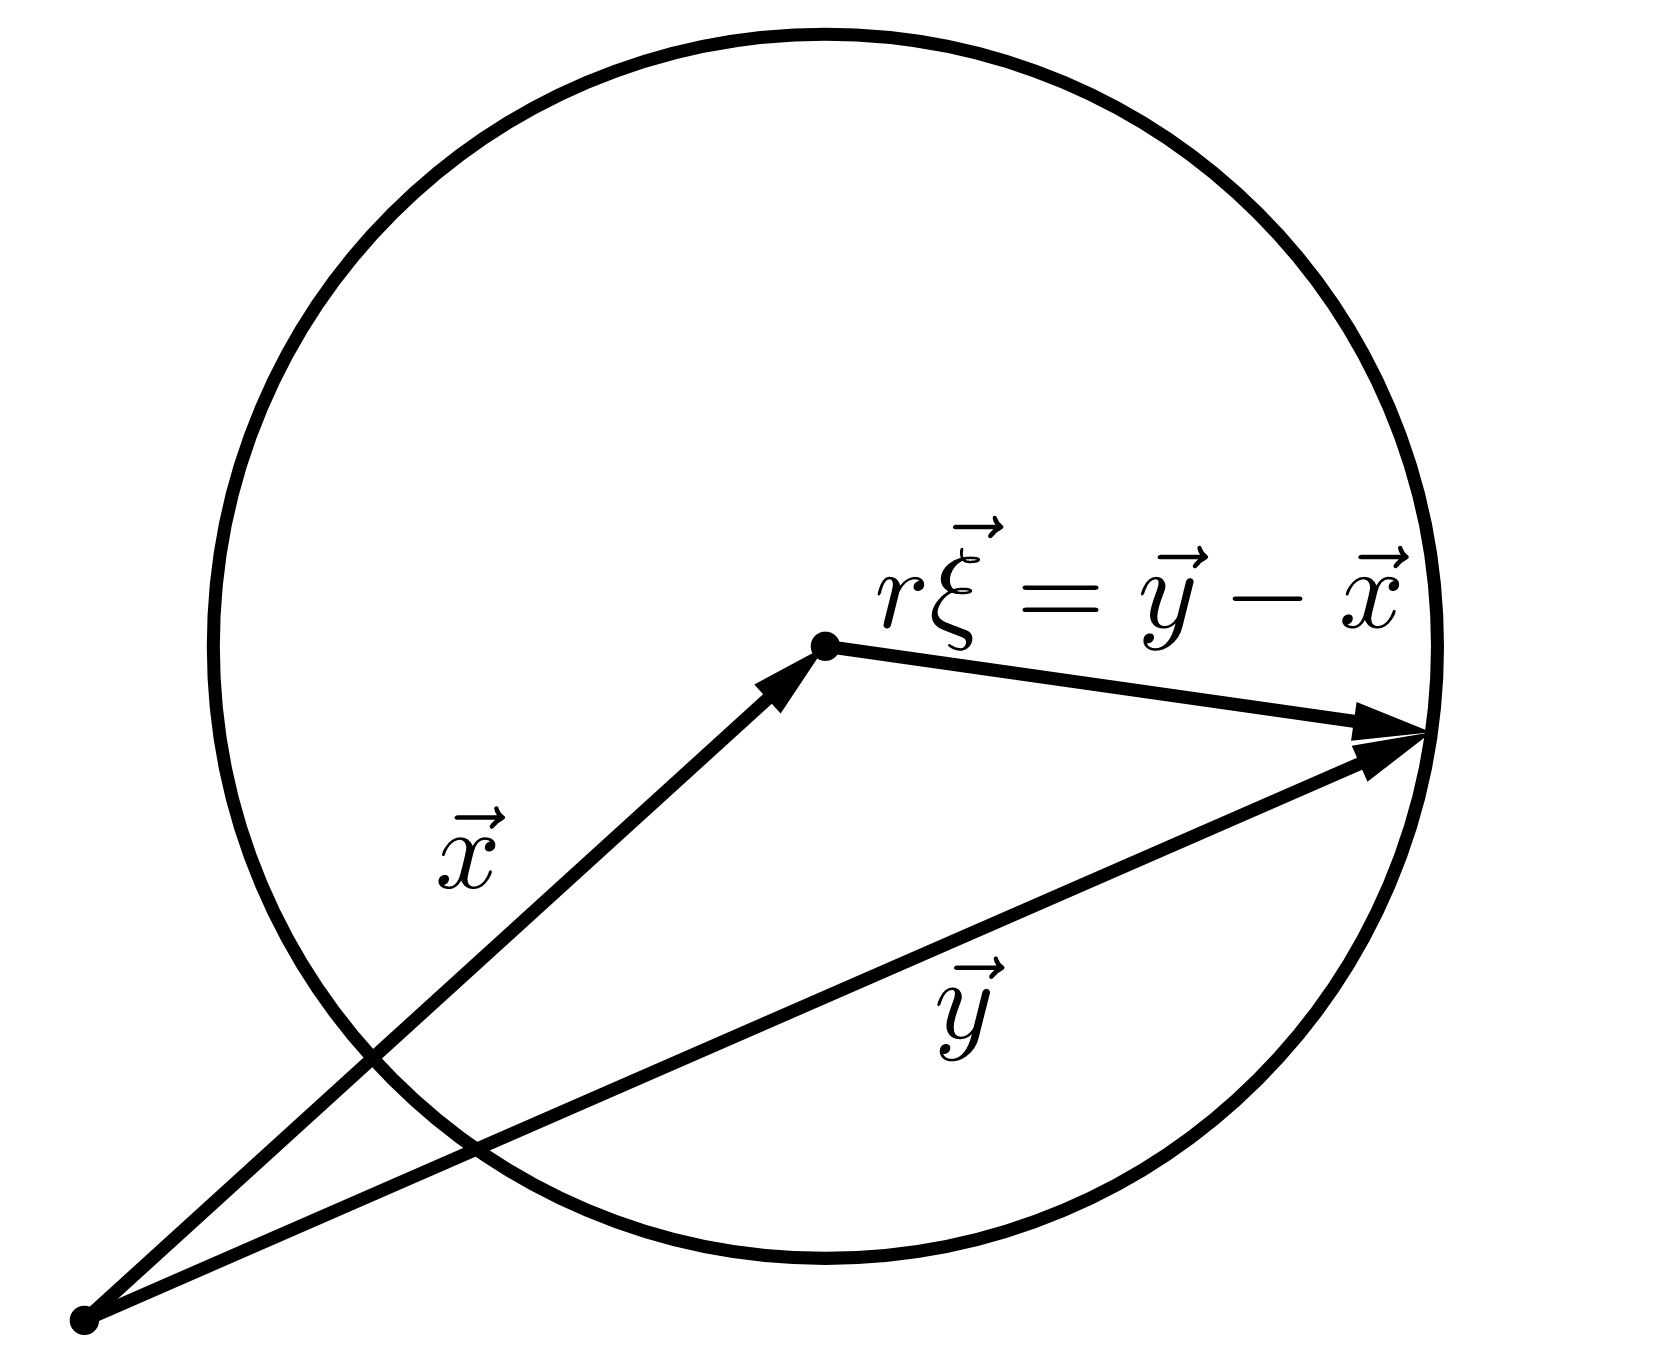
\includegraphics[scale=0.1]{xi.png}
\end{center}
\[
    y-x = \xi r    
\]
\begin{equation}
y = x + \xi r
\end{equation}
\[
    |y-x| = |\xi|r = r \quad,\quad |\xi| = 1    
\]
Thus the surface elements are related as.
\[
    dS_y = r^{n-1} dS_\xi    
\]
Substituting in (1)
\begin{equation}
M_{f}(x,r) = \frac{1}{\omega_{n}} \int_{|\xi|=1} f(x+\xi r)dS_\xi
\end{equation} 
At $r = 0$
\begin{equation}
M_{f}(x,0) = \frac{f(x)}{\omega_{n}} \int_{|\xi|=1} dS_\xi = f(x)
\end{equation}
The integral $\displaystyle \int_{|\xi|=1} dS_\xi$ is the surface area of a unit sphere in n dimensions which is equal to $\omega_n$
\\
From (3) and remembering that $y$, $x$, and $\xi$ are all vectors, then we can write their components as
\[
    y_i = x_i + \xi_i r    
\]
Using this vector notation to differentiate (4) with respect to r.
\begin{align*}
\frac{\partial M_f (x,r)}{\partial r} &= \frac{1}{\omega_n} \int_{|\xi|=1} \frac{\partial f(y)}{\partial r}dS_\xi
\\
&= \frac{1}{\omega_n} \int_{|\xi|=1} \sum_{i=1}^{n} \frac{\partial f(y)}{\partial y_i}\frac{\partial y_i}{\partial r} dS_\xi
\\
&= \frac{1}{\omega_n} \int_{|\xi|=1} \sum_{i=1}^{n} \frac{\partial f(y)}{\partial y_i}\xi_i dS_\xi
\end{align*}
Using the chain rule we find.$\displaystyle \frac{\partial f(y)}{\partial y_i} \frac{\partial x_i}{\partial x_i} = \frac{\partial f(y)}{\partial y_i} \frac{\partial y_i}{\partial x_i}\frac{\partial x_i}{\partial y_i} = \frac{\partial f(y)}{\partial x_i}$, since $\displaystyle \frac{\partial x_i}{\partial y_i} = 1$
\[
    \frac{\partial M_f (x,r)}{\partial r} = \frac{1}{\omega_n} \int_{|\xi|=1} \sum_{i=1}^{n} \frac{\partial f(y)}{\partial x_i}\xi_i dS_\xi    
\]
Using the chain rule one more time.$\displaystyle \frac{\partial f(y)}{\partial x_i} \frac{\partial \xi_i}{\partial \xi_i}= \frac{\partial f(y)}{\partial x_i}\frac{\partial x_i}{\partial \xi_i}\frac{\partial \xi_i}{\partial x_i} = \frac{\partial f(y)}{\partial \xi_i}\frac{1}{r}$, since $\displaystyle \frac{\partial \xi_i}{\partial x_i} = \frac{1}{r}$
\begin{equation}
\frac{\partial M_f (x,r)}{\partial r} = \frac{1}{\omega_n r} \int_{|\xi|=1} \sum_{i=1}^{n} \frac{\partial f(y)}{\partial \xi_i}\xi_i dS_\xi
\end{equation}
\begin{theorem}[Divergence Theorem]
    Also called Green-Gauss-Ostrogradsky theorem relates the volume integral to the surface integral under some conditions, more precisely, the surface integral of a vector field over a closed surface (flux) is equal to the volume integral of the divergence over the region. We will use this later in our treatment.
    \[
        \int\int\int_{Volume} \frac{\partial \textbf{F}(x,y,z)}{\partial x}dV = \int\int_{Surface} \textbf{F}(x,y,z)\cos(\angle x,\vec{n}) dS    
    \]
    Or in general.
    \[
        \int\int\int_{Volume} \nabla \cdot \textbf{F} dV = \int\int_{Surface} \textbf{F}\cdot \vec{n} dS
    \]
\end{theorem}

Comparing the form we have with the divergence theorem we see that the sum we have is the dot product of our vector function with $\xi$
which is the unit vector always normal to the surface of the sphere by our definition, and we can transform our integral to a volume integral.
\begin{enrichment*}{}
    The components $\xi_i$ are direction cosines, i.e $\xi_{1}^{2}+\xi_{2}^{2}+...+\xi_{n}^{2} = 1$
\end{enrichment*}
\[
    \frac{\partial M_f (x,r)}{\partial r} = \frac{1}{\omega_n r} \int_{|\xi|\leq 1} \sum_{i=1}^{n} \frac{\partial^2 f(y)}{\partial \xi_{i}^{2}} d\xi    
\]
Using the chain rule we have.
\begin{align*}
\frac{\partial M_f (x,r)}{\partial r} &= \frac{r^2}{\omega_n r} \int_{|\xi|\leq 1} \sum_{i=1}^{n} \frac{\partial^2 f(y)}{\partial x_{i}^{2}} d\xi
\\
&=\frac{r}{\omega_n} \nabla_{x}^{2} \int_{|\xi|\leq 1} f(y)d\xi
\end{align*}
Notice that .
\[
    \frac{\partial M_f (x,0)}{\partial r} = 0    
\]
Now we will change our volume element from the relation (3).
\begin{enrichment*}{}
    Remember that y is a vector thus $dy = dy_1 dy_2 dy_3 ...dy_n$ and since $dy_i = rd\xi_i$ 
    \\
    Then $dy = rrr...d\xi_1 d\xi_2 d\xi_3 ...$
\end{enrichment*}
\[
    d\xi = \frac{1}{r^n}dy    
\]
Thus we have 
\begin{align*}
\frac{\partial M_f (x,r)}{\partial r} &= \frac{r}{\omega_n r^n} \nabla_{x}^{2} \int_{|y-x|\leq r} f(y)dy
\\
&= \frac{1}{\omega_n r^{n-1}} \nabla_{x}^{2} \int_{|y-x|\leq r} f(y)dy
\\
&= \frac{1}{\omega_n r^{n-1}} \nabla_{x}^{2} \int_{\rho = 0}^{r} \int_{|y-x| = \rho} f(y)dS_y d\rho
\end{align*}
Rearranging and multiply and divide by $\rho^{n-1}$.
\[
    r^{n-1} \frac{\partial M_f (x,r)}{\partial r} =  \nabla_{x}^{2}\int_{\rho = 0}^{r} \rho^{n-1}\frac{1}{\omega_n \rho^{n-1}} \int_{|y-x|= \rho}f(y)dS_y d\rho    
\]
Notice that on the right hand side an expression the same as the spherical mean (4) is attained thus we substitute .
\[
    r^{n-1} \frac{\partial M_f (x,r)}{\partial r} = \nabla_{x}^{2}\int_{\rho = 0}^{r} \rho^{n-1} M_{f}(x,\rho) d\rho    
\]
Differentiating the expression with respect to r.
\begin{align*}
\frac{\partial}{\partial r}\left( r^{n-1} \frac{\partial M_f (x,r)}{\partial r}\right) &= \nabla_{x}^{2} \frac{\partial}{\partial r}\int_{\rho = 0}^{r} \rho^{n-1} M_{f}(x,r) d\rho
\\
r^{n-1} \frac{\partial^2 M_f (x,r)}{\partial r^2} + (n-1)r^{n-2}\frac{\partial M_f (x,r)}{\partial r} &= \nabla_{x}^{2} r^{n-1} M_f (x,r)
\end{align*}
Rearranging and simplifying we finally arrive at Darboux's equation (2) where $ V=M_f (x,r) $.
\[
    \frac{\partial^2 M_f (x,r)}{\partial r^2} + \frac{n-1}{r} \frac{\partial M_f (x,r)}{\partial r} = \nabla_{x}^{2} M_f (x,r)    
\]
\newpage
\setcounter{equation}{0}
\subsection{Kirchhoff's Formula}
We have seen how formula d'Almbert can solve the one dimensional wave equation Cauchy problem but the solution of the wave equation in dimensions higher than one shows to be more complicated. 
Our attempt to solve the three dimensional wave equation 
we will use the results of the spherical mean and Darboux's equation to develop an effective formula to solve three dimensional wave equation Cauchy problems called Kircchoff's formula.
\par
\begin{figure*}[b]
    \begin{minipage}[h]{\textwidth}
    \begin{enrichment}{Gustav Kirchhoff}{Kirchhoff.jpg}{2.4}{.8}{.17}
        Gustav Kirchhoff (1824-1887) was a prominent German physicist
        Kirchhoff made significant advancements in the understanding of wave phenomena and the mathematical modeling of physical systems using PDEs.
        One of Kirchhoff's most notable contributions in PDEs is his formulation of the Kirchhoff equations, which describe the propagation of waves in elastic materials, such as solids and thin plates. These equations are fundamental to the study of vibrations, acoustics, and the behavior of mechanical systems subjected to dynamic loads.
    \end{enrichment}    
\end{minipage}
\end{figure*}
Consider the following three dimensional wave equation Cauchy problem.
\begin{equation}
    \begin{cases}
        \displaystyle \frac{\partial^2 u(x,t)}{\partial t^2} = c^2 \nabla_{x}^{2}u(x,t) \quad,\quad c\neq 0 \quad,\quad t > 0
        \\
        \text{I.C} \quad \Longrightarrow \quad 
        \begin{cases}
            u\left(x,0 \right) = \phi\left(x\right)
            \\
            \displaystyle \frac{\partial u\left(x,0 \right)}{\partial t} = \psi\left(x\right)
        \end{cases} 
    \end{cases}
\end{equation}
where $x = (x_1,x_2,x_3)$ is a three dimensional vector.
\par
we start by considering Darboux's equation in n = 3.
\begin{align}
\frac{\partial^2 M_f (x,r)}{\partial r^2} + \frac{2}{r} \frac{\partial M_f (x,r)}{\partial r} &= \nabla_{x}^{2} M_f (x,r) \notag
\\ 
r\frac{\partial^2 M_f (x,r)}{\partial r^2} + 2 \frac{\partial M_f (x,r)}{\partial r} &= r\nabla_{x}^{2} M_f (x,r)
\end{align}
we notice that.
\begin{align*}
\frac{\partial }{\partial r}\left(rM_f (x,r) \right) &= r\frac{\partial M_f(x,r)}{\partial r} +M_f (x,r)
\\
\frac{\partial^2 }{\partial r^2}\left(rM_f (x,r) \right) &= r\frac{\partial^2 M_f(x,r)}{\partial r^2} + \frac{\partial M_f(x,r)}{\partial r}  + \frac{\partial M_f(x,r)}{\partial r}
\end{align*}
\begin{equation}
\frac{\partial^2 }{\partial r^2}\left(rM_f (x,r) \right) = r\frac{\partial^2 M_f(x,r)}{\partial r^2} + 2\frac{\partial M_f(x,r)}{\partial r}
\end{equation}
substituting (3) in (2).
\begin{equation}
\frac{\partial^2 }{\partial r^2}\left(rM_f (x,r) \right) = r\nabla_{x}^{2} M_f (x,r)
\end{equation}
we now consider the spherical mean of the function $u$ where n = 3 then $\omega_3 = 4\pi$ the surface area of a 3d sphere
\[
    M_{u}(x,t,r) = \frac{1}{4\pi r^2} \int_{|y-x|=r} f(y)dS_y    
\]
calculating the spherical mean of the whole equation (1) we get.
\[
    \frac{\partial^2}{\partial t^2} M_{u}(x,t,r) = c^2 \nabla_{x}^{2}M_{u}(x,t,r)    
\]
multiply by r.
\[
    \frac{\partial^2}{\partial t^2} r M_{u}(x,t,r) = c^2 r\nabla_{x}^{2}M_{u}(x,t,r)    
\]
from (4) we get.
\begin{equation}
    \frac{\partial^2}{\partial t^2} \left[r M_u (x,t,r) \right] = c^2 \frac{\partial^2 }{\partial r^2}\left[r M_u (x,t,r) \right]    
\end{equation} 
the initial conditions will be.
\begin{equation}
rM_{u}(x,0,r) = rM_\phi(x,r) = \frac{r}{4\pi r^2} \int_{|y-x|=r}\phi(y)dS_y
\end{equation}
\begin{equation}
\frac{\partial}{\partial t}\left(rM_{u}(x,0,r)\right) = rM_\psi(x,r) = \frac{r}{4\pi r^2} \int_{|y-x|=r}\psi(y)dS_y
\end{equation}
we notice that this is a one dimensional wave equation 
\[
    \begin{cases}
        \displaystyle \frac{\partial^2}{\partial t^2} \left[r M_u (x,t,r) \right] = c^2 \frac{\partial^2 }{\partial r^2}\left[r M_u (x,t,r) \right]    
        \\
        \text{I.C} \quad \Longrightarrow \quad 
        \begin{cases}
            rM_{u}(x,0,r) = rM_\phi(x,r)
            \\
            \frac{\partial}{\partial t}\left(rM_{u}(x,0,r)\right) = rM_\psi(x,r)
        \end{cases}
    \end{cases}
\]
that can be solved using the method developed earlier d'Alembert formula.
\[
    rM_u(x,t,r) = \frac{1}{2}\left[(r+ct)M_\phi(x,r+ct)+(r-ct)M_\phi(x,r-ct)\right]+\frac{1}{2c}\int_{r-ct}^{r+ct} sM_\psi(x,s)ds    
\]
\begin{equation}
M_u(x,t,r) = \frac{1}{2r}\left[(r+ct)M_\phi(x,r+ct)+(r-ct)M_\phi(x,r-ct)\right]+\frac{1}{2cr}\int_{r-ct}^{r+ct} sM_\psi(x,s)ds
\end{equation}
we note that.
\[
\lim_{r\to 0} M_u(x,t,r) = u(x,t)    
\]
now we start studying the limit to find our target function $u(x,t)$.
\begin{align}
\lim_{r\to 0} M_u(x,t,r) = \lim_{r\to 0}\frac{1}{2r}\left[(r+ct)M_\phi(x,r+ct)+(r-ct)M_\phi(x,r-ct)\right] \notag
\\
+\lim_{r\to 0}\frac{1}{2cr}\int_{r-ct}^{r+ct} sM_\psi(x,s)ds
\end{align}
the first limit can be rearranged to.
\[
    \lim_{r\to 0} \frac{1}{2r}\left[rM_\phi(x,r+ct)+ctM_\phi(x,r+ct)+rM_\phi(x,r-ct)-ctM_\phi(x,r-ct)\right]    
\]
rearranging one more time and noting that the spherical mean function is an even function 
\\
$\displaystyle M_f(r)=M_f(-r)$ thus we can multiply the $r$ variable by negative one.
\begin{align*}
    \lim_{r\to 0} \frac{1}{2r}\left[rM_\phi(x,r+ct)+rM_\phi(x,r-ct)\right] & +\lim_{r\to 0} \frac{1}{2r}ct\left[M_\phi(x,r+ct)-M_\phi(x,ct-r)\right]
    \\
    \frac{1}{2} \lim_{r\to 0} \left[M_\phi(x,r+ct)+M_\phi(x,r-ct)\right] & + ct \lim_{r\to 0} \frac{\left[M_\phi(x,r+ct)-M_\phi(x,ct-r)\right]}{2r}
    \\
    \frac{1}{2} \left[M_\phi(x,ct)+M_\phi(x,-ct)\right] & + ct \frac{\partial M_\phi(x,ct)}{\partial ct}
\end{align*}
the first limit is equal to $M_\phi(x,ct)$ due to the function being even and we notice that the second limit is the definition of the derivative$\displaystyle f'(x) = \lim_{h\to 0} \frac{f(x+h) - f(x-h)}{2h}$ with respect to $ct$ thus the limit is finally evaluated to.
\[
    \lim_{r\to 0}\frac{1}{2r}\left[(r+ct)M_\phi(x,r+ct)+(r-ct)M_\phi(x,r-ct)\right] = M_\phi(x,ct) + ct\frac{\partial}{\partial ct}(M_\phi(x,ct))    
\]
consider .
\[
    \frac{\partial}{\partial t}[tM_\phi(x,ct)] = M_\phi(x,ct)+t \frac{\partial M_\phi(x,ct)}{\partial ct}\frac{\partial ct}{\partial t} = M_\phi(x,ct)+ct \frac{\partial M_\phi(x,ct)}{\partial ct}    
\]
\[
\therefore \lim_{r\to 0}\frac{1}{2r}\left[(r+ct)M_\phi(x,r+ct)+(r-ct)M_\phi(x,r-ct)\right] = \frac{\partial}{\partial t}[tM_\phi(x,ct)]    
\]
now considering the second limit.
\[
    \lim_{r\to 0}\frac{1}{2cr}\int_{r-ct}^{r+ct} sM_\psi(x,s)ds    
\]
direct substitution will result in an undetermined form $\frac{0}{0}$ since the function inside the integral is an odd function thus the symmetrical integral will vanish thus we will utilize l'Hopital's rule to find the limit.
\begin{enrichment*}{l'Hopital's rule}
    \[
        \lim_{{x \to c}} \frac{{f(x)}}{{g(x)}} = \lim_{{x \to c}} \frac{{f'(x)}}{{g'(x)}}    
    \]
\end{enrichment*}
\[
    \lim_{r\to 0}\frac{1}{2cr}\int_{r-ct}^{r+ct} sM_\psi(x,s)ds = \lim_{r\to 0}\frac{1}{2c}\frac{\partial}{\partial r}\left[\int_{r-ct}^{r+ct} sM_\psi(x,s)ds\right]    
\]
to find the derivative of the integral we use Libenz rule.
\begin{enrichment*}{Libenz rule}
    \[
        \frac{d}{dx}\int_{a(x)}^{b(x)} f(x,y)dy = \frac{db(x)}{dx}f(x,b(x))-\frac{da(x)}{dx}f(x,a(x)) + \int_{a(x)}^{b(x)} \frac{\partial f(x,y)}{\partial x} dy    
    \]
\end{enrichment*}
in our case
\begin{align*}
\frac{\partial}{\partial r}\left[\int_{r-ct}^{r+ct} sM_\psi(x,s)ds\right] &= (r+ct)M_\psi(x,r+ct) - (r-ct)M_\psi(x,r-ct) + \int_{r-ct}^{r+ct} \frac{\partial}{\partial r} sM_\psi(x,s)ds
\\
 &= ct[M_\psi(x,r+ct)+M_\psi(x,r-ct)]
\end{align*}
\\
thus the limit will become.
\[
    \lim_{r\to 0}\frac{1}{2cr}\int_{r-ct}^{r+ct} sM_\psi(x,s)ds = \lim_{r\to 0}\frac{ct[M_\psi(x,r+ct)+M_\psi(x,r-ct)]}{2c}    
\]
which is finally evaluated to.
\[
    \lim_{r\to 0}\frac{1}{2cr}\int_{r-ct}^{r+ct} sM_\psi(x,s)ds = tM_\psi(x,ct)    
\]
we now finally substitute the first and the second limit in (10).
\[
    u(x,t) = \lim_{r\to 0} M_u(x,t,r) = \frac{\partial}{\partial t}[tM_\phi(x,ct)] + tM_\psi(x,ct)    
\]
using the definition of spherical mean with $r=ct$ our final formula becomes.
\[
    u(x,t) = \frac{\partial}{\partial t}\left[\frac{1}{4\pi c^2 t}\int_{|y-x|=ct}\phi(y)dS_y\right] + \frac{1}{4\pi c^2 t}\int_{|y-x|=ct}\psi(y)dS_y    
\]
which is called Kirchhoff's Formula.

\newpage
\section{Laplace's Equation}
Laplace's equation is one of the most important PDE in mathematical physics most notably in the study of electromagnetism.
and it's in the form of:
\[
    \nabla^2 u(x,y)= \frac{\partial^2 u(x,y)}{\partial x^2}+\frac{\partial^2 u(x,y)}{\partial y^2} = 0 \quad,\quad (x,y) \in G    
\]
Where G is a simply bounded connected domain whose boundary $\gamma$ is a simple closed contour.
\begin{center}
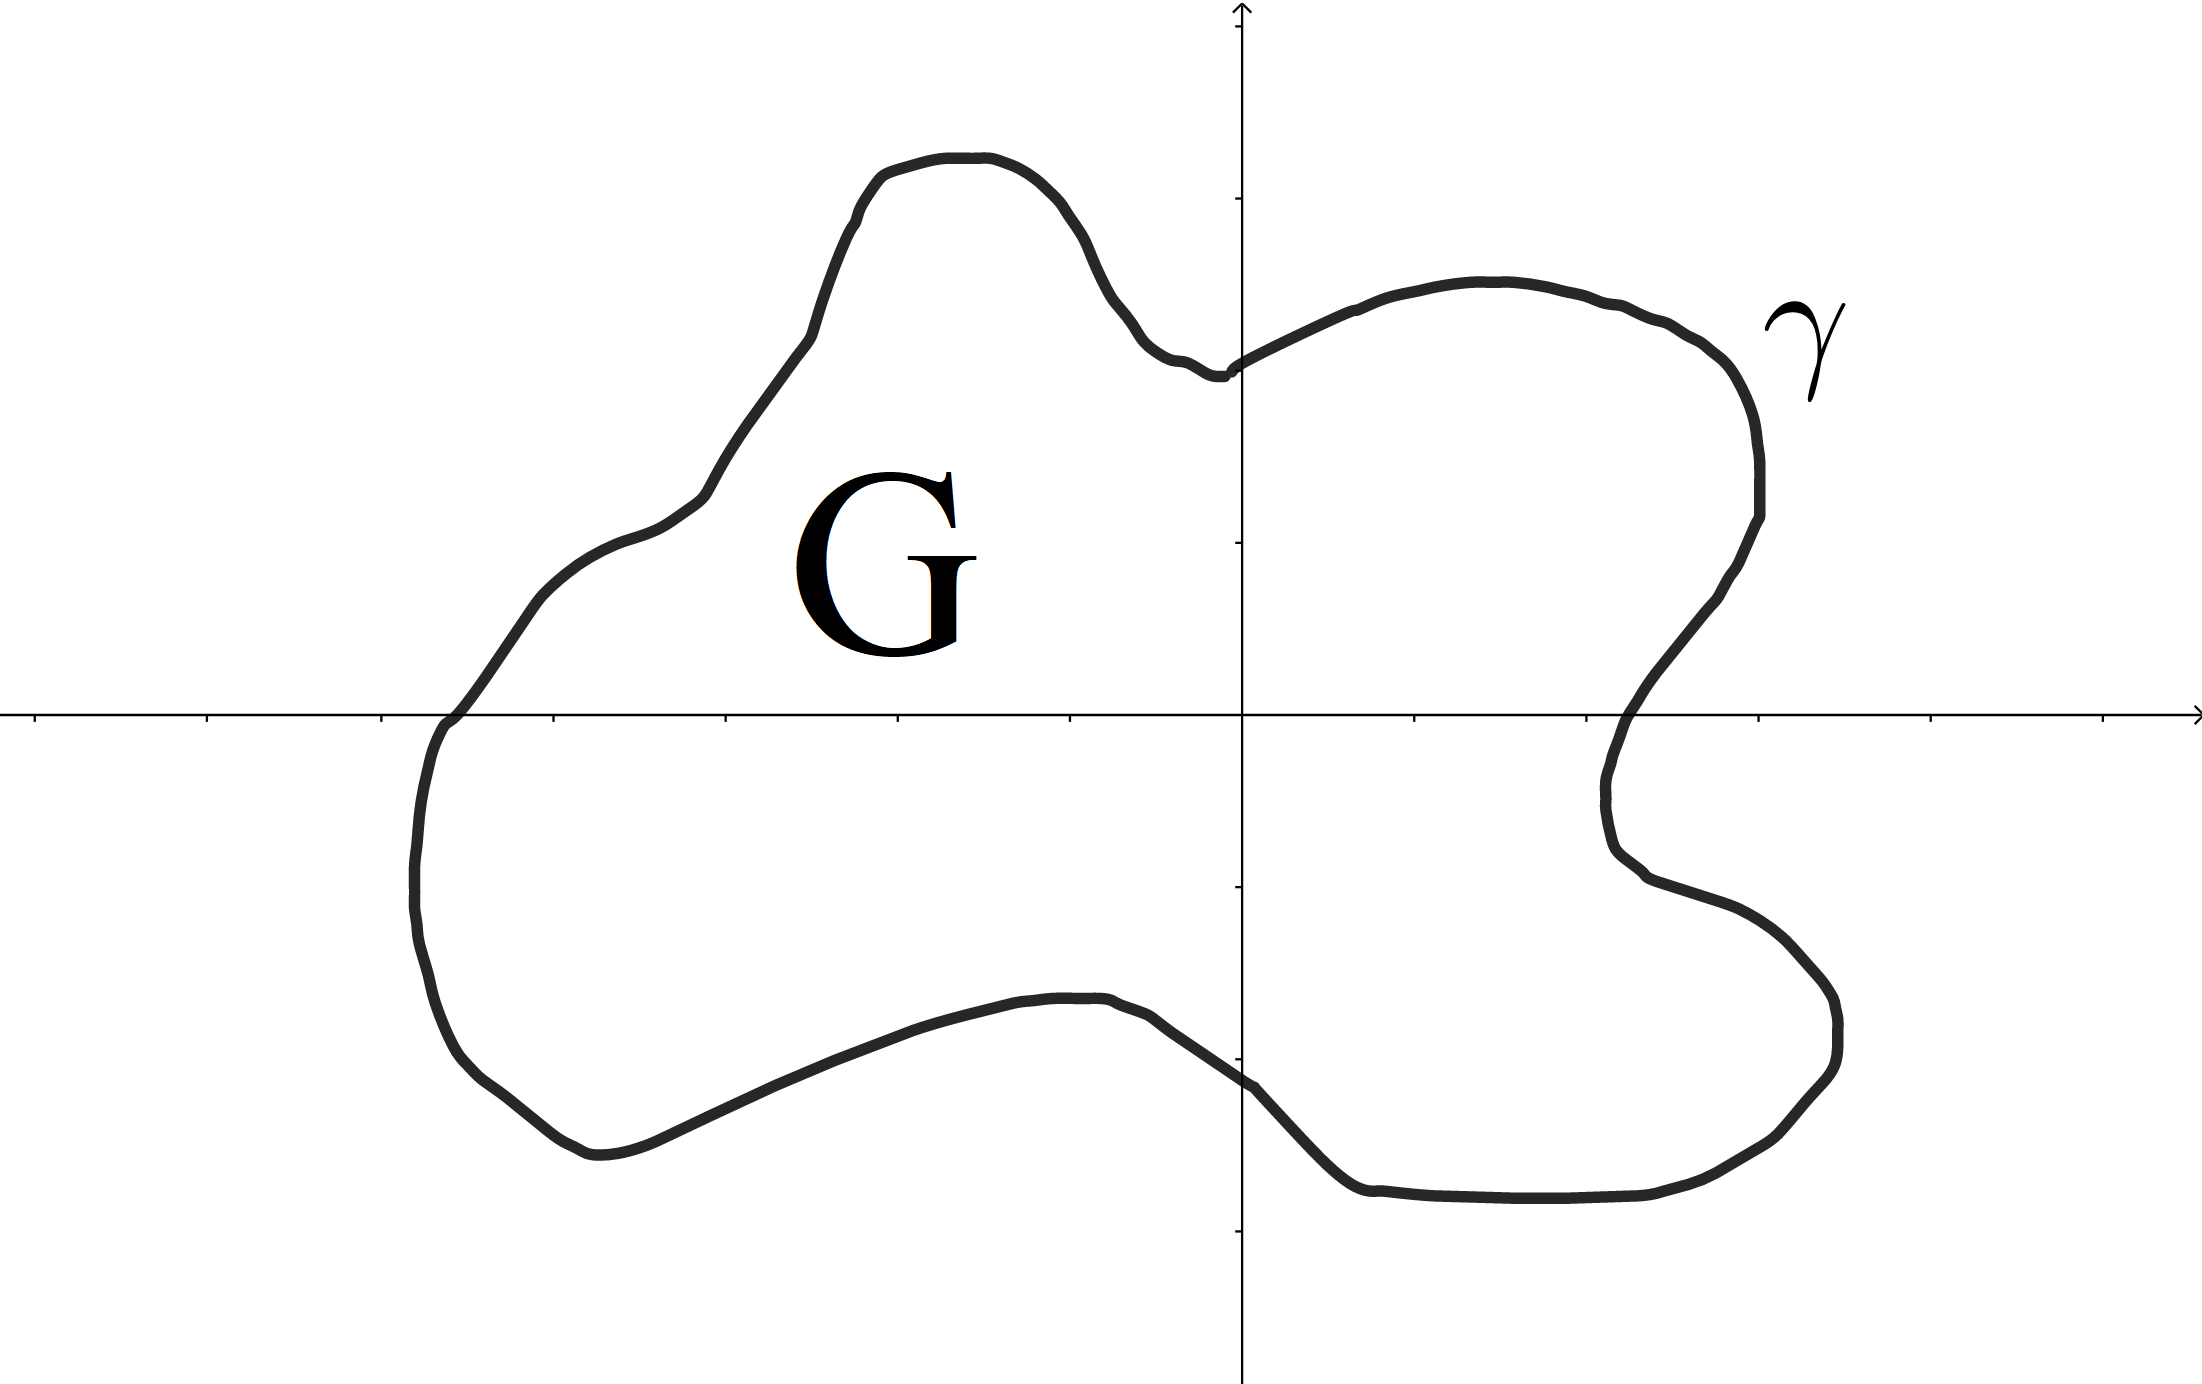
\includegraphics[scale=0.1]{domain.png}
\end{center}
If the function $u$ that satisfy the Laplace equation and is in the set of two dimensional continuous functions on the domain G , $u \in C^2(G)$, 
i.e. all of $\displaystyle u, \frac{\partial u}{\partial x}, \frac{\partial u}{\partial y}, \frac{\partial^2 u}{\partial x^2},\frac{\partial^2 u}{\partial y^2}$,
are continuous functions on G, then the function $u$ is called a harmonic function on G.
\setcounter{equation}{0}
\subsection{Solution of Laplace's Equation on a Circle}

Consider the following Dirichlet problem
\begin{equation}
    \begin{cases}
        \displaystyle \nabla^2 u(x,y) = \frac{\partial^2 u(x,y)}{\partial x^2} + \frac{\partial^2 u(x,y)}{\partial y^2} = 0 \quad,\quad \forall (x,y) \in G
        \\
        \text{I.C} \quad \Longrightarrow \quad u(x,y)|_\gamma = f(x,y)
    \end{cases}
\end{equation}
\begin{center}
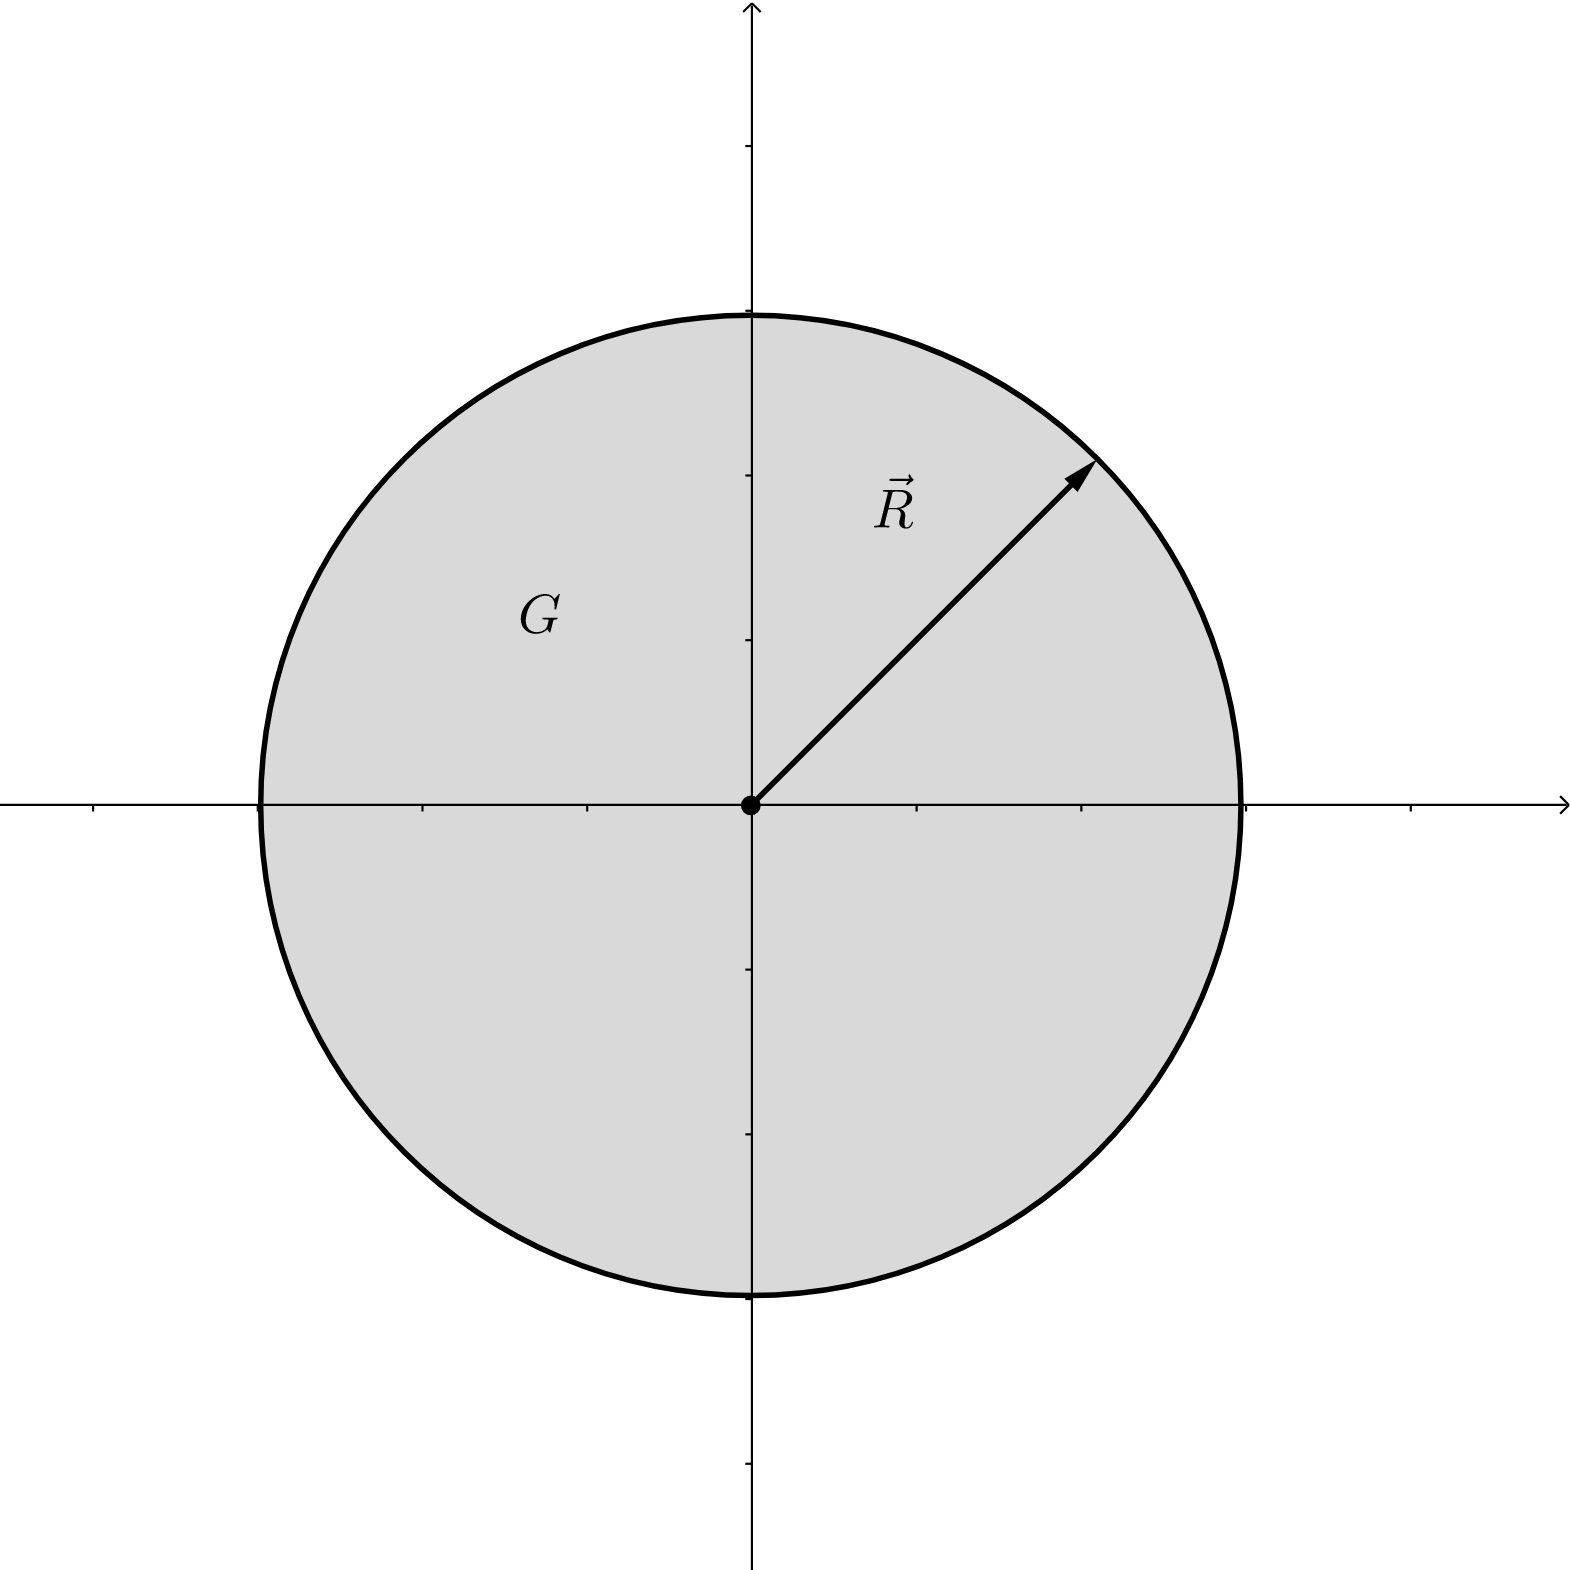
\includegraphics[scale=0.14]{circle.png}
\end{center}
\begin{align*}
G &:= \left\lbrace (x,y):x^2+y^2 < R^2 \right\rbrace
\\
\gamma &:= \left\lbrace (x,y):x^2+y^2 = R^2 \right\rbrace
\end{align*}
By putting $x = r cos(\theta)$ and $y = r sin(\theta)$ and recreate equation (1) using chain rule we can express it as.
\[
    r^2 \frac{\partial^2 u(r,\theta)}{\partial r^2} + r \frac{\partial u(r,\theta)}{\partial r} + \frac{\partial^2 u(r,\theta)}{\partial \theta^2} = 0    
\]
The derivatives of $r$ and $\theta$ can be separated thus utilizing the separation of variables method.
\begin{align*}
u(r,\theta) &= V(r)F(\theta)
\\
\frac{\partial u}{\partial r} &= \frac{d V(r)}{dr}F(\theta)
\\
\frac{\partial^2 u}{\partial r^2} &= \frac{d^2 V(r)}{dr^2}F(\theta)
\\
\frac{\partial^2 u}{\partial \theta^2} &= V(r)\frac{d^2 F(\theta)}{d\theta^2}
\end{align*}
Therefore we get.
\begin{figure*}[b]
    \begin{minipage}[h]{\textwidth}
    \begin{enrichment}{Laplace}{Laplace.jpg}{2.4}{.8}{.17}
        Pierre Simon Laplace (1749-1827) was a French mathematician, astronomer, and physicist 
        In the context of PDEs, Laplace's most influential contributions stem from his work in mathematical physics and celestial mechanics. One of his fundamental achievements was in the development of the theory of potential, where he used PDEs to study the behavior of gravitational and electric fields. Laplace's pioneering work laid the foundation for the study of potential theory and its applications in various branches of science and engineering.
    \end{enrichment}    
\end{minipage}
\end{figure*}
\begin{equation}
r^2F(\theta)\frac{d^2 V(r)}{dr^2} +rF(\theta)\frac{d V(r)}{dr} + V(r)\frac{d^2 F(\theta)}{d\theta^2} = 0
\end{equation}
Dividing (2) by $V(r)F(\theta)$ we get.
\begin{equation}
\frac{r^2}{V(r)}\frac{d^2 V(r)}{dr^2} +\frac{r}{V(r)}\frac{d V(r)}{dr} + \frac{1}{F(\theta)}\frac{d^2 F(\theta)}{d\theta^2} = 0
\end{equation}
\[
    \frac{r^2}{V(r)}\frac{d^2 V(r)}{dr^2} +\frac{r}{V(r)}\frac{d V(r)}{dr} = n^2 = -\frac{1}{F(\theta)}\frac{d^2 F(\theta)}{d\theta^2}    
\]
We start solving for the $F(\theta)$. 
\[
    \frac{d^2 F(\theta)}{d\theta^2} = -n^2F(\theta)    
\]
The solution will be. 
\begin{equation}
F(\theta) = A cos(n\theta)+B sin(n\theta)
\end{equation}
Then solving for $V(r)$.
\[
r^2\frac{d^2 V(r)}{dr^2} +r\frac{d V(r)}{dr} = n^2V(r)    
\]
By putting $r = e^t$
\begin{align*}
\frac{dV(r)}{dr} &= \frac{dV(r)}{dt}\frac{dt}{dr} = e^{-t} \frac{dV(r)}{dt} \quad\Rightarrow  r \frac{dV(r)}{dr}=\frac{dV(r)}{dt}
\\
\frac{d^2V(r)}{dr^2} &= \frac{d}{dr}\left[e^{-t} \frac{dV(r)}{dt}\right]
\\
&=  \frac{d}{dt}\left[e^{-t} \frac{dV(r)}{dt}\right] \frac{dt}{dr} 
\\
&= \frac{d}{dt}\left[e^{-t} \frac{dV(r)}{dt}\right] e^{-t}
\\
&= e^{-2t}\left[-\frac{dV(r)}{dt}+\frac{d^2V(r)}{dt^2}\right] \quad \Rightarrow \quad r^2\frac{d^2V(r)}{dr^2} = \frac{d^2V(r)}{dt^2}-\frac{dV(r)}{dt}
\end{align*}
Substituting will result in.
\begin{align*}
\frac{d^2V(r)}{dt^2}-\frac{dV(r)}{dt}+\frac{dV(r)}{dt}&=n^2V(r)
\\
\frac{d^2V(r)}{dt^2} &= n^2V(r)
\end{align*}
\[
\therefore V(r) = Ce^{nt}+De^{-nt} = Cr^n+Dr^{-n}    
\]
To maintain the continuity of the function we put D=0.
\[
\therefore V(r) = Cr^n
\]
Substituting V and F in u.
\begin{equation}
u(r,\theta) = r^n[A cos(n\theta)+B sin(n\theta)]
\end{equation}
From this the boundary condition becomes a function only in $\theta$.
\begin{equation}
u|_\gamma = H(\theta)
\end{equation}
Taking the sum of all solutions we get.
\[
    u(r,\theta) = a_o + \sum_{n=1}^{\infty} r^n[a_n cos(n\theta)+b_n sin(n\theta)]    
\]
At $\gamma \longrightarrow $ r = 1.
\[
    H(\theta) = a_o + \sum_{n=1}^{\infty} a_n cos(n\theta)+b_n sin(n\theta) 
\]
Then we find the Fourier coefficients.
\begin{align*}
a_o &= \frac{1}{2\pi}\int_{0}^{2\pi} H(\psi ) d\psi 
\\
a_n &=\frac{1}{\pi}\int_{0}^{2\pi} H(\psi ) cos(n\psi ) d\psi 
\\
a_n &=\frac{1}{\pi}\int_{0}^{2\pi} H(\psi ) \sin(n\psi ) d\psi 
\end{align*}
Then we get.
\begin{align*}
u(r,\theta) &= \frac{1}{2\pi}\int_{0}^{2\pi} H(\psi ) d\psi  + \frac{1}{\pi}\sum_{n=1}^{\infty} r^n \int_{0}^{2\pi} H(\psi )[\cos(n\psi )\cos(n\theta) + \sin(n\psi )\sin(n\theta)]d\psi 
\\
u(r,\theta) &= \frac{1}{2\pi}\int_{0}^{2\pi} H(\psi ) d\psi  + \frac{1}{\pi}\sum_{n=1}^{\infty}r^n\int_{0}^{2\pi} H(\psi )\cos[n(\psi  - \theta)]d\psi 
\end{align*}
\begin{enrichment*}{}
    $\cos[A-B] = \cos(A)\cos(B) + \sin(A)\sin(B)$
\end{enrichment*}
From the value of the exponential series we can get.
\[
    S_1 = \sum_{n=1}^{\infty} r^n \cos(n\phi),\quad S_2 =\sum_{n=1}^{\infty}r^n \sin(n\phi), \quad \phi = \psi  - \theta    
\]
\[
    S_1 + i S_2 = \sum_{n=0}^{\infty} r^n e^{in\phi}    
\]
This is the form of a geometric series the value of the summation is
\[
    \sum_{n=0}^{\infty} r^n e^{in\phi} = \frac{r e^{i\phi}}{1- r e^{i\phi}}
\]
We now manipulate the expression to obtain the real part.
\newpage
\begin{align*}
\hspace{4cm}
\frac{r^n e^{i\phi}}{1- r^n e^{i\phi}} &= \frac{r(cos\phi+isin\phi)}{1-r(cos\phi+isin\phi)}
\\
&= \frac{r(cos\phi+isin\phi)}{(1-rcos\phi)-irsin\phi} \cdot \frac{(1-rcos\phi)+irsin\phi}{(1-rcos\phi)+irsin\phi}
\\
&= \frac{rcos\phi - r^2 + ir \sin\phi}{1-2rcos\phi+r^2}
\\
&= \frac{rcos\phi - r^2}{1-2rcos\phi+r^2} + i \frac{\sin\phi}{1-2rcos\phi+r^2}
\end{align*}
We find that.
\[
    S_1 = \frac{rcos\phi - r^2}{1-2rcos\phi+r^2}    
\]
Substituting in the expression for $u$ we get.
\begin{align*}
u(r,\theta) &= \frac{1}{2\pi}\int_{0}^{2\pi} H(\psi ) d\psi  + \frac{1}{\pi}\int_{0}^{2\pi} H(\psi )\frac{rcos(\psi  -\theta) - r^2}{1-2rcos(\psi  -\theta)+r^2}d\psi 
\\
            &= \frac{1}{2\pi}\int_{0}^{2\pi} H(\psi )\frac{2rcos(\psi  -\theta) - 2r^2+1-2rcos(\psi  -\theta)+r^2}{1-2rcos(\psi  -\theta)+r^2}d\psi 
\end{align*}
Simplify.
\[
    u(r,\theta) = \frac{1}{2\pi}\int_{0}^{2\pi} H(\psi )\frac{1-r^2}{1-2rcos(\psi  -\theta)+r^2}d\psi     
\]
And for a circle of radius $R$ we get Poisson's Formula.
\[
    u(r,\theta) = \frac{1}{2\pi R}\int_{0}^{2\pi R} H(\beta)\frac{R^2-r^2}{R^2-2Rrcos(\psi  -\theta)+r^2}d\beta \quad, \quad \beta = R\psi     
\]
We can easily find $u$ in terms of $x$ and $y$, the two forms are equivalent.
\subsection{Harmonic Functions}
We will discuss some properties or theorems of the harmonic function
\begin{observation}
    $u(x,y)$ at the center of the circle where $r=0$ that is when $x=0$ and $y=0$ is
    \[
        u(0,0) = \frac{1}{2\pi R}\int_{0}^{2\pi R} H(\beta)\frac{R^2-(0)^2}{R^2-2R(0)cos(\psi  -\theta)+(0)^2}d\beta =\frac{1}{2\pi R}\int_{0}^{2\pi R} H(\beta)d\beta     
    \]
\end{observation}    
\begin{theorem}[Liouville Theorem]
    A harmonic function of the whole plane, i.e. $(x,y) \in \mathbb{R}^2$, can not be bounded from above or bounded from below unless it is constant.    
\end{theorem}
\begin{proof}[\textcolor{theme}{Proof}]
    Assume the harmonic function is bounded from below, i.e.    
    \[
        u(x,y) \geq m \quad,\quad \forall (x,y) \in \mathbb{R}^2     
    \]
    Without loss of generality $m > 0$ is assumed.
    \\
    We know that $ -1 \leq \cos(\theta) \leq 1$
    \begin{align*}
        \therefore
        \frac{R^2-r^2}{R^2+2Rr+r^2} &\leq \frac{R^2-r^2}{R^2-2Rrcos(\psi  -\theta)+r^2} \leq \frac{R^2-r^2}{R^2-2Rr+r^2}
        \\
        \frac{(R-r)(R+r)}{{(R+r)}^2} &\leq \frac{R^2-r^2}{R^2-2Rrcos(\psi  -\theta)+r^2} \leq \frac{(R-r)(R+r)}{{(R-r)}^2}
        \\
        \frac{R-r}{R+r} &\leq \frac{R^2-r^2}{R^2-2Rrcos(\psi  -\theta)+r^2} \leq \frac{R+r}{R-r}
    \end{align*}
    Therefore
    \[
        \frac{1}{2\pi R}\int_{0}^{2\pi R} H(\beta)\frac{R-r}{R+r} d\beta \leq \frac{1}{2\pi R}\int_{0}^{2\pi R} H(\beta)\frac{R^2-(0)^2}{R^2-2R(0)cos(\psi  -\theta)+(0)^2}d\beta \leq \frac{1}{2\pi R}\int_{0}^{2\pi R} H(\beta)\frac{R+r}{R-r} d\beta    
    \]
    And from observation 5.1 
    \[
        \frac{R-r}{R+r} u(0,0) \leq u(x,y) \leq \frac{R+r}{R-r} u(0,0)    
    \]
    Taking the limit as $R \to \infty$ to include the whole plane we get.
    \[
        u(0,0) \leq u(x,y) \leq u(0,0) \quad \Rightarrow \quad u(x,y) = u(0,0)    
    \]
    Therefore the function is constant when it is bounded from below, the same argument can be used for bounded from above case.
\end{proof}

\begin{theorem}[Regularity Theorem]
    If $u$ is a harmonic and continuous function on $G$ and its boundary $\gamma$, then $u$ is analytic at every point on $G$, i.e. can be represented as as a power series and can be differentiated infinite times.    
\end{theorem}
\begin{proof}[\textcolor{theme}{Proof}]
    We know that.       
    \[
        u(x,y) = \frac{a_o}{2} + \sum_{n=1}^{\infty} r^n[a_n \cos(n\theta)+b_n \sin(n\theta)]    
    \]
    And we know from de Moivre's formula that.
    \[
        \cos(n\theta) = \sum_{k=0}^{n} A_k {(\cos\theta)}^k {(\sin\theta)}^{n-k}    
    \]
    And
    \[
        \sin(n\theta) =  \sum_{k=0}^{n} B_k {(\cos\theta)}^k {(\sin\theta)}^{n-k}    
    \]
    Substituting in $u(x,y)$ we get.
    \[
        u(x,y) = \frac{a_o}{2} + \sum_{n=1}^{\infty} r^n\left[a_n\sum_{k=0}^{n} A_k (cos\theta)^k (sin\theta)^{n-k}\right] + \sum_{n=1}^{\infty} r^n\left[b_n\sum_{k=0}^{n} B_k (cos\theta)^k (sin\theta)^{n-k}\right]    
    \]
    Put $r^n = r^{n-k}r^k $ and we know that $x = rcos\theta$ and $y=rsin\theta$.
    \[
        u(x,y) = \frac{a_o}{2} + \sum_{n=1}^{\infty}\sum_{k=0}^{n} a_n A_k x^k y^{n-k} + \sum_{n=1}^{\infty}\sum_{k=0}^{n}b_n B_k x^k y^{n-k}    
    \]
    \[
        u(x,y) = \frac{a_o}{2} + \sum_{n=1}^{\infty}\sum_{k=0}^{n} C_{n,k} x^k y^{n-k}
    \]
    Therefore the function can be represented as a power series at any point, i.e. is analytical.
\end{proof}
\begin{figure*}[b]
    \begin{minipage}[h]{\textwidth}
    \begin{enrichment*}{Analytic Function}
        Is a Function that can be represented by a convergent power series in a region around each point within its domain. It is a function that is differentiable at every point within this region, and its derivative exists everywhere in that domain. 
        and it can be differentiated nth time for $n \in \mathbb{N}$
        \\
        Example (any Polynomial functions , Exponential function , Trigonometric functions ,etc.)
    \end{enrichment*}        
\end{minipage}
\end{figure*}
\newpage
\setcounter{equation}{0}
\subsection{Green's Identity}
We will study Green's integral in three dimensions but it can be also applied to $n^{\text{th}}$ dimensions.
\begin{center}
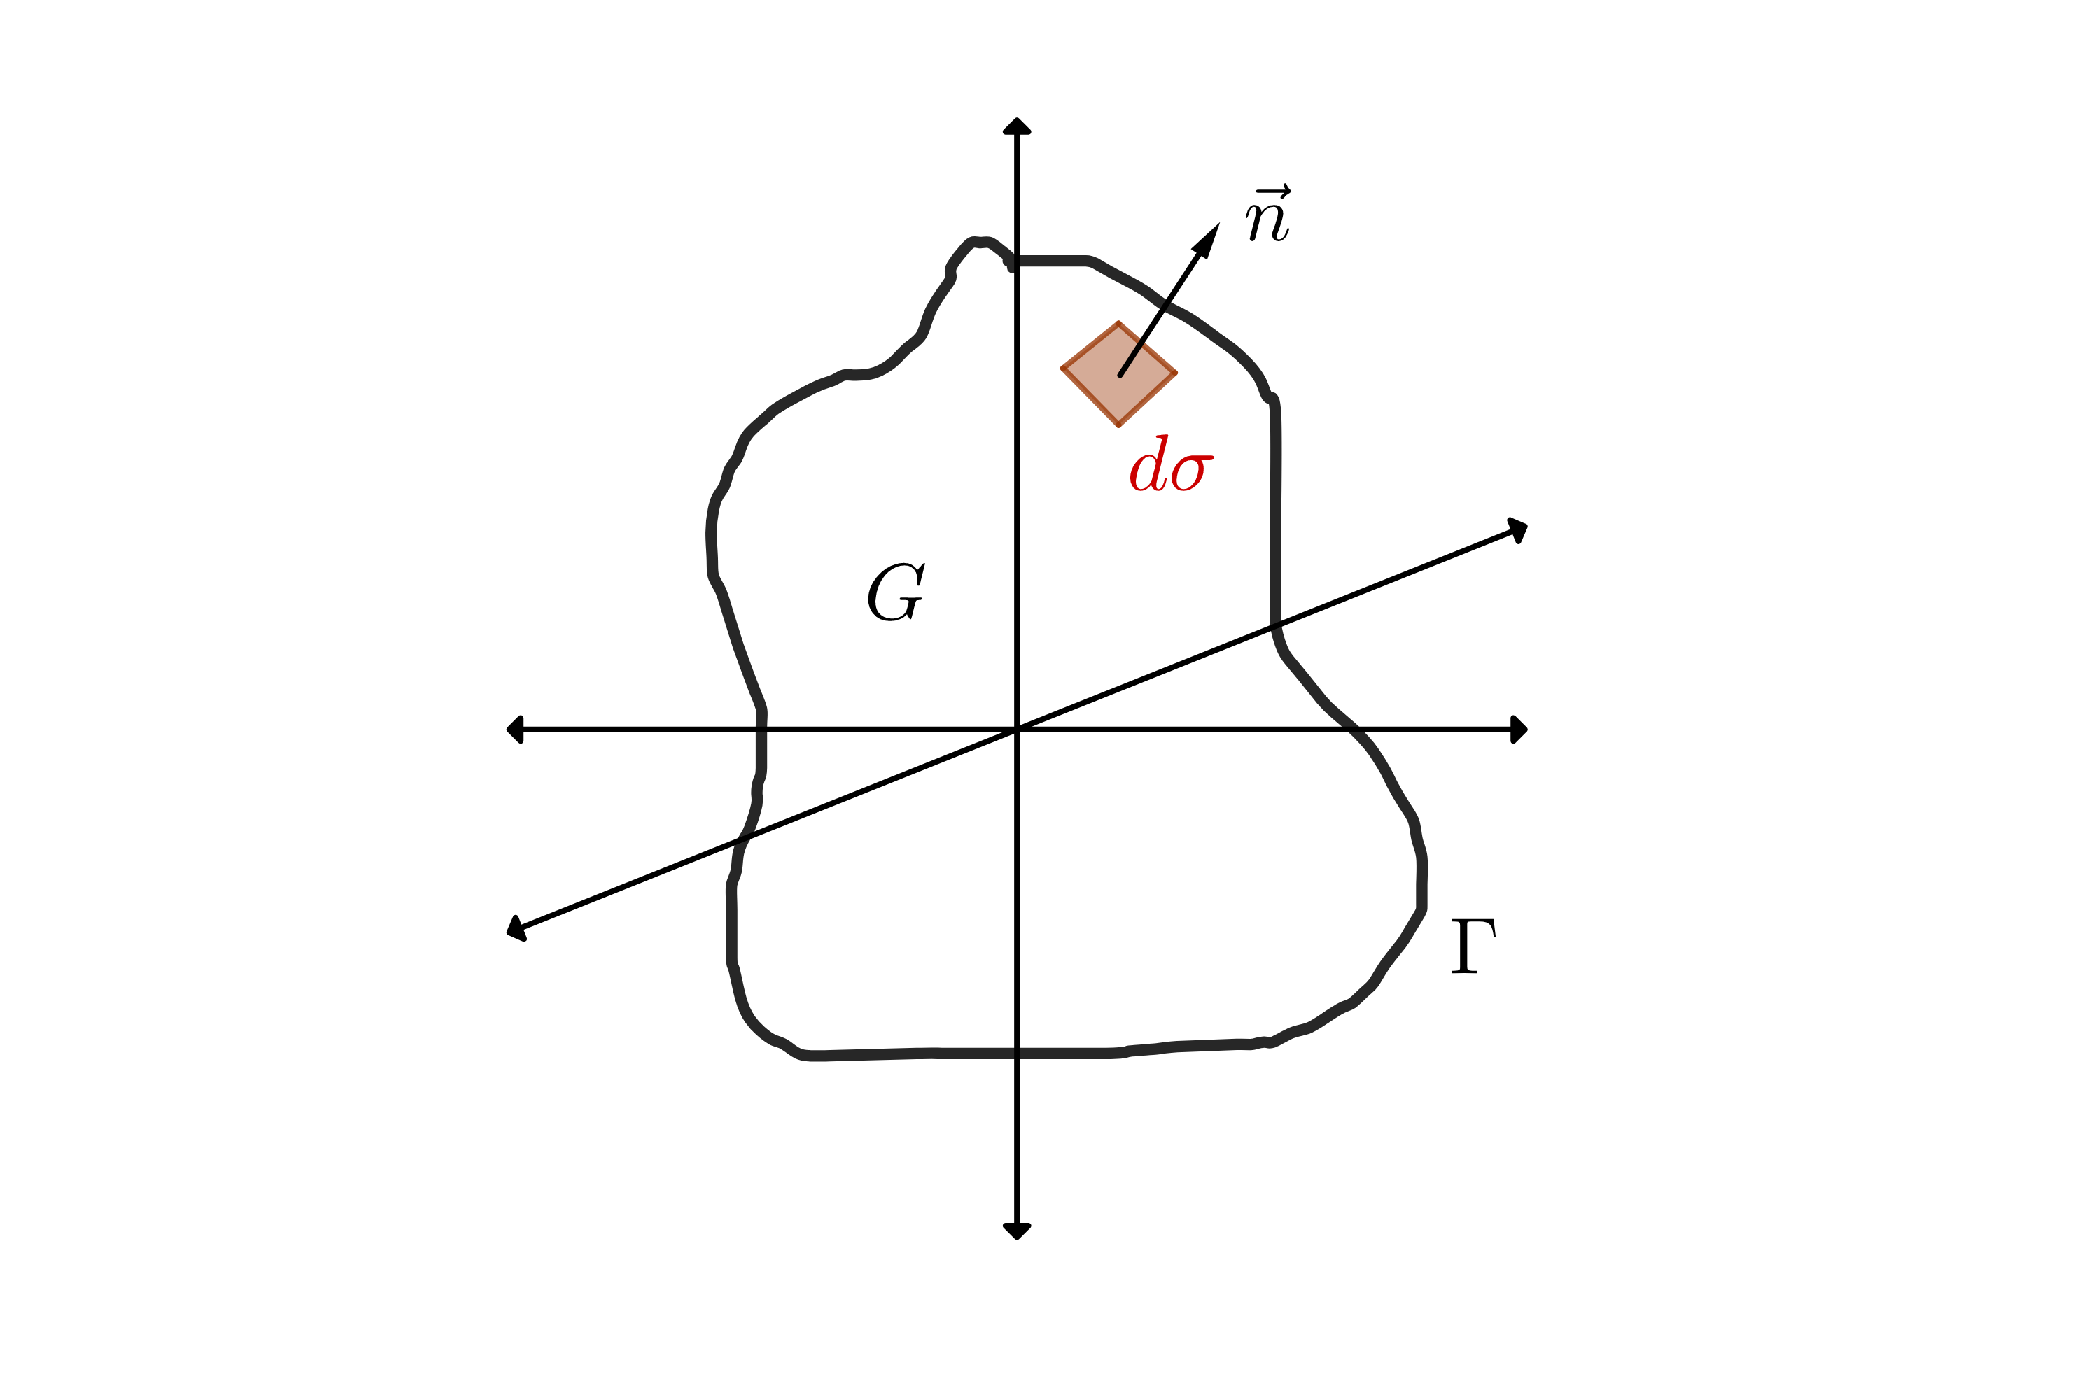
\includegraphics[scale=0.2]{green.png}
\end{center}
For any domain $G$ in three dimensions with boundary $\Gamma$, where the volume element is
\\
$dx = dx_1 dx_2 dx_3$, the surface element is $d\sigma$, and $\vec{n}$ is the normal to the surface, let $v(x_1,x_2,x_3)$, $u(x_1,x_2,x_3)$ be functions such that $v,u\in C^3(G)$ and $v,u\in C^2(G\cup \Gamma)$.
\par
Now we start our treatment by studying the following differentiation. 
\begin{align*}
\frac{\partial }{\partial x_i}\left(v\frac{\partial u}{\partial x_i}\right) &= v\frac{\partial^2 u}{\partial x_{i}^{2}} + \frac{\partial v}{\partial x_i}\frac{\partial u}{\partial x_i}
\\
v\frac{\partial^2 u}{\partial x_{i}^{2}} &= \frac{\partial }{\partial x_i}\left(v\frac{\partial u}{\partial x_i}\right) - \frac{\partial v}{\partial x_i}\frac{\partial u}{\partial x_i}
\end{align*}
Integrating over volume.
\[
    \int_G v\frac{\partial^2 u}{\partial x_{i}^{2}} dx = \int_G \frac{\partial }{\partial x_i}\left(v\frac{\partial u}{\partial x_i}\right) dx - \int_G \frac{\partial v}{\partial x_i}\frac{\partial u}{\partial x_i} dx    
\]
From the divergence theorem we can transform the first integral on the right hand side to a surface integral.
\[
    \int_G v\frac{\partial^2 u}{\partial x_{i}^{2}} dx = \int_\Gamma v\frac{\partial u}{\partial x_i}cos(\vec{n},x_i) d\sigma - \int_G \frac{\partial v}{\partial x_i}\frac{\partial u}{\partial x_i} dx    
\]
Summing over i.
\begin{align}
\int_G v\sum_{i=1}^{3}\frac{\partial^2 u}{\partial x_{i}^{2}} dx &= \int_\Gamma v\sum_{i=1}^{3}\frac{\partial u}{\partial x_i}cos(\vec{n},x_i) d\sigma - \sum_{i=1}^{3}\int_G \frac{\partial v}{\partial x_i}\frac{\partial u}{\partial x_i} dx 
\nonumber
\\ 
\int_G v\nabla^2 u dx &= \int_\Gamma v\frac{\partial u}{\partial \vec{n}} d\sigma - \sum_{i=1}^{3}\int_G \frac{\partial v}{\partial x_i}\frac{\partial u}{\partial x_i} dx
\end{align}
In the same manner we can find.
\begin{equation}
\int_G u\nabla^2 v dx = \int_\Gamma u\frac{\partial v}{\partial \vec{n}} d\sigma - \sum_{i=1}^{3}\int_G \frac{\partial u}{\partial x_i}\frac{\partial v}{\partial x_i} dx
\end{equation}
Subtracting (2) from (1) results in.
\[
    \int_G \left[v\nabla^2 u - u\nabla^2 v\right]dx = \int_\Gamma \left[v\frac{\partial u}{\partial \vec{n}}-u\frac{\partial v}{\partial \vec{n}}\right] d\sigma    
\]
This equation is Green's Identity.

\begin{theorem}[Oleinik's Theorem (maximum principle)]
    If $u(x,y)$ is a harmonic function on G and $u(x,y)$ is continuous on $G \cup \gamma$, then $u(x,y)$ attains its maximum or minimum value on $\gamma$    
\end{theorem}
\begin{proof}[\textcolor{theme}{Proof}]
    Suppose that the maximum value of u on $G \cup \gamma$ is M, and the minimum value of u on $G \cup \gamma$ is m, then it is clear that $M \geq m$.
    \par
    We want to proof that $M = m$ 
    \par
    Suppose that $M > m$ 
    \par
    We first define
    \[
        v(x,y) = u(x,y) + \frac{M-m}{2d^2}\left[(x-x_{1})^2+(y-y_{1})^2\right]    
    \]
    \begin{center}
        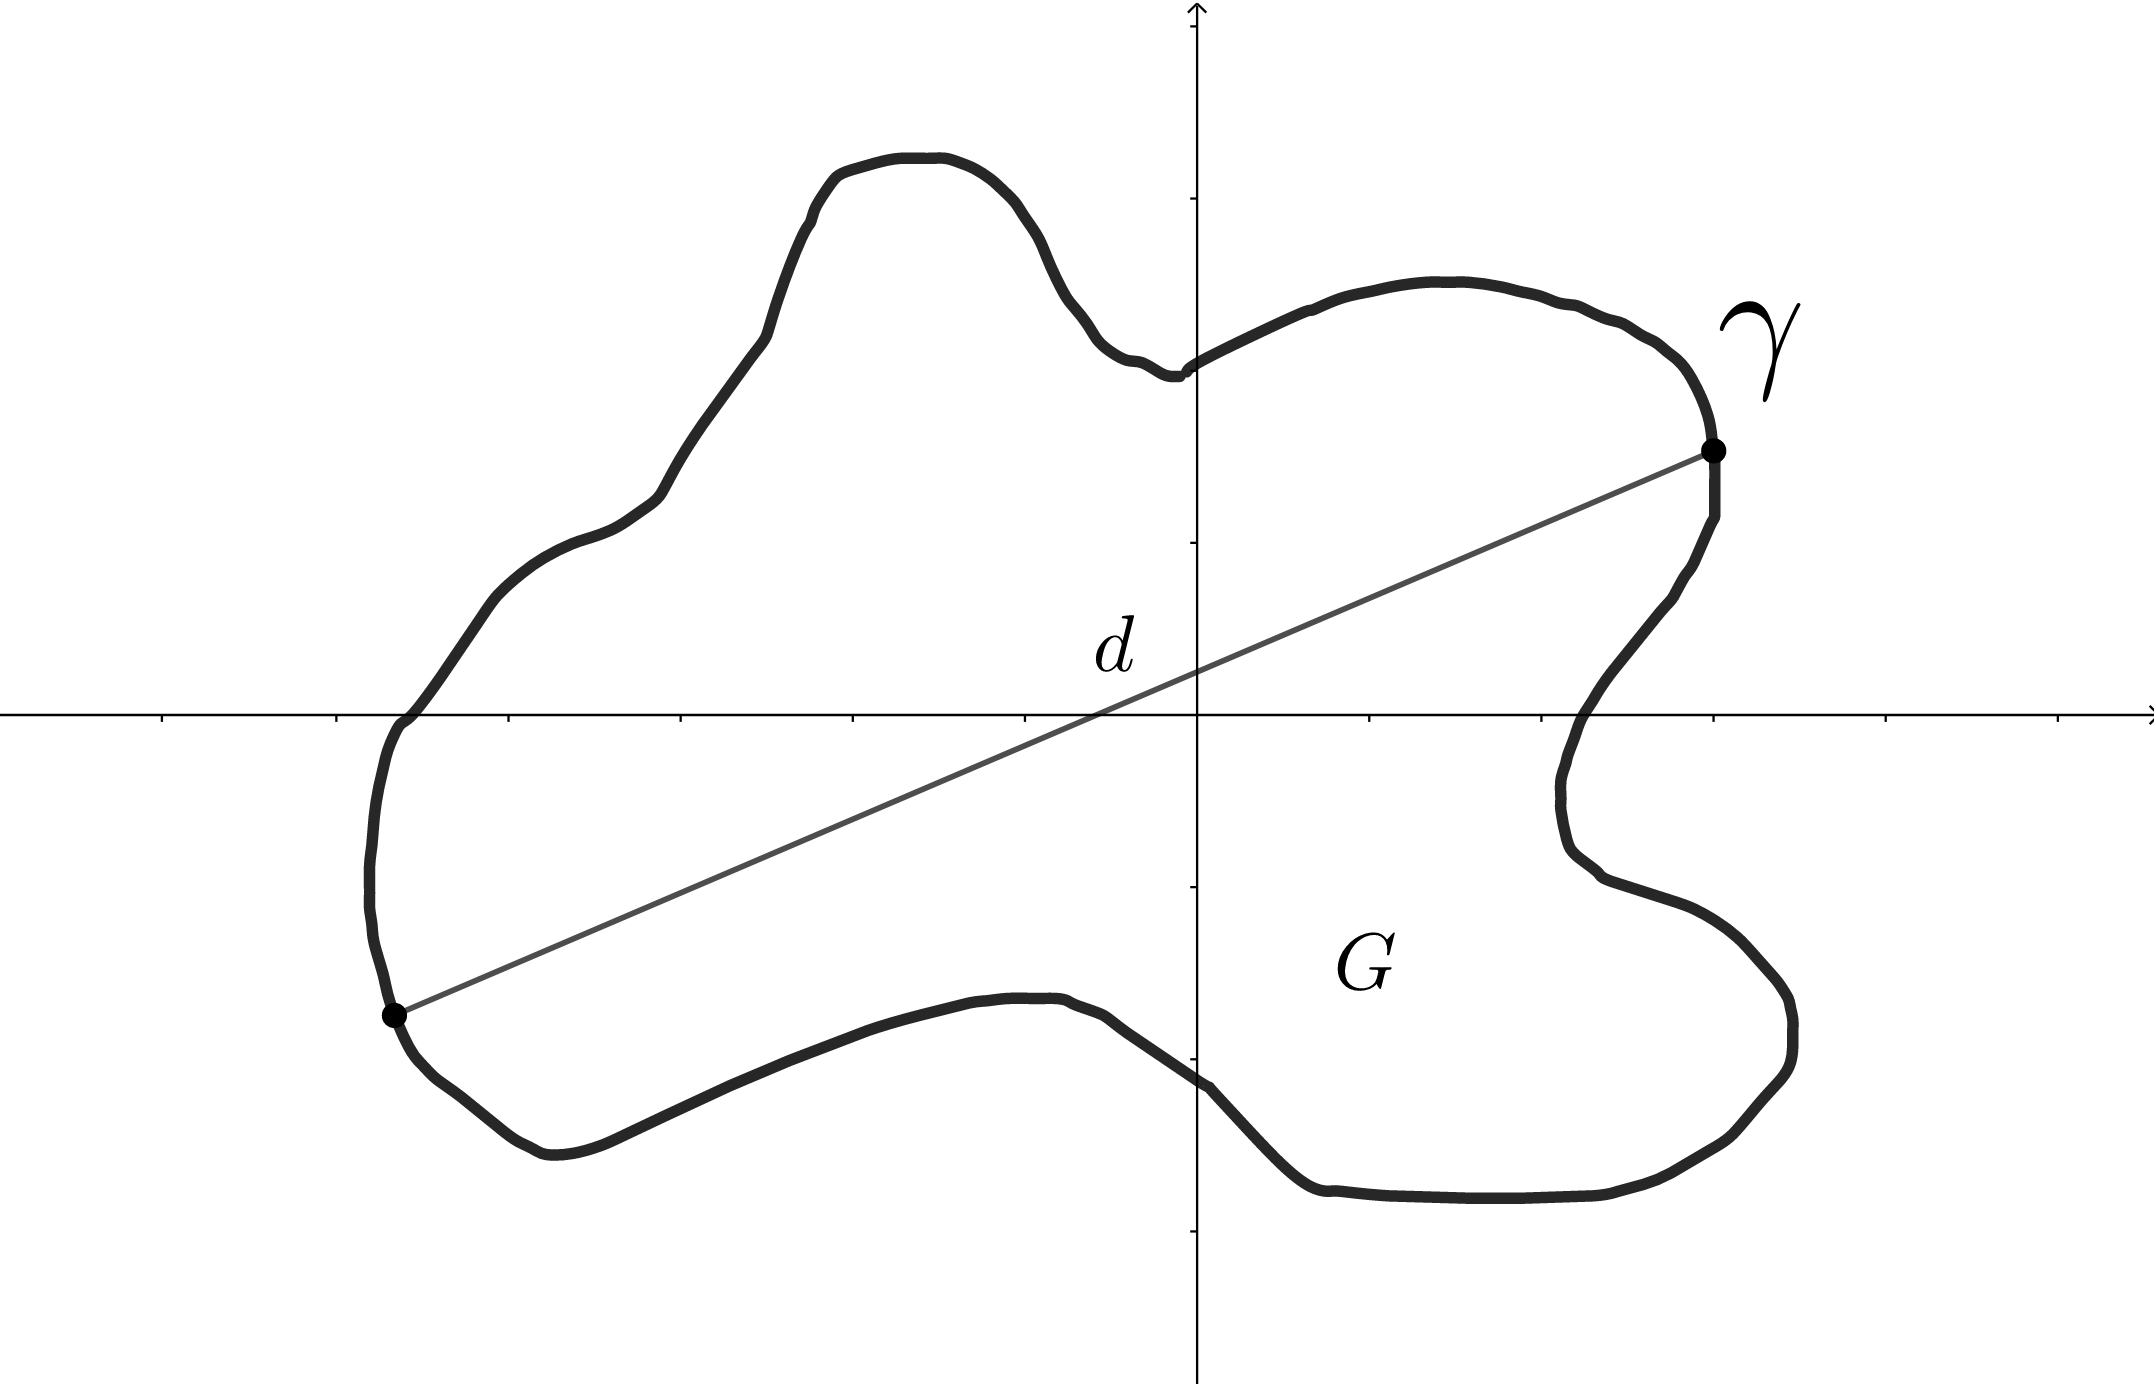
\includegraphics[scale=0.1]{diameter.png}
    \end{center}
    Where d is the diameter of the domain G or the longest distance between two point, 
    and $(x_1,y_1)$ is a point inside G such that, $u(x_1,y_1) = M$, thus we have.
    \[
        v(x_1,y_1) = u(x_1,y_1) = M    
    \]
    And on $\gamma$ we find
    \begin{align*}
        v(x,y) &\leq m+\frac{M-m}{2}
        \\
        &\leq \frac{M+m}{2} < \frac{M+M}{2}
        \\
        &< M
    \end{align*}
    This means that $v$ attains a maximum value at a point call it $(x_2,y_2)$ inside G thus we have.
    \[
        \frac{\partial^2 v(x_2,y_2)}{\partial x^2} \leq 0 \quad \text{and} \quad \frac{\partial^2 v(x_2,y_2)}{\partial y^2} \leq 0    
    \]
    \setcounter{equation}{0}
    \begin{equation}
        \therefore  \nabla^2 v(x_2,y_2) =  \frac{\partial^2 v(x_2,y_2)}{\partial x^2}+\frac{\partial^2 v(x_2,y_2)}{\partial y^2} \leq 0
    \end{equation}
    From the definition of v we obtain
    \begin{align*}
        \frac{\partial^2 v}{\partial x^2} &= \frac{\partial^2 u}{\partial x^2} + \frac{M-m}{d^2}
        \\
        \frac{\partial^2 v}{\partial y^2} &= \frac{\partial^2 u}{\partial y^2} + \frac{M-m}{d^2}
        \\
        \nabla^2 v = \frac{\partial^2 v}{\partial x^2} + \frac{\partial^2 v}{\partial x^2} &= \nabla^2 u + \frac{2(M-m)}{d^2}
        \\
        \because u(x,y) &\text{ is harmonic}\dquad \Longrightarrow \therefore \nabla^2 u = 0
        \\\tag{2}
        \nabla^2 v &= \frac{2(M-m)}{d^2} > 0 
    \end{align*}
    Which is a contradiction from (1) and (2)
    \\
    Therefore M must equal m 
\end{proof}
\begin{theorem}[Uniqueness of Dirichlet Problem]
    If there exist a solution of Laplace's equation 
    with a boundary condition (Dirichlet problem)
    \[
    \exists u \in C^2(G) \quad,\quad u \in C(G \cup \gamma) \quad,\quad \text{such that} \quad \nabla^2 u =0 \quad \text{and} \quad u|_\gamma = f
    \]
    Then the solution is unique.
\end{theorem}
\begin{proof}[\textcolor{theme}{Proof}]
Assuming the two function $u_1$ and $u_2$ are harmonic functions on G with boundary $\gamma$, i.e. 
\begin{align*}
    u_1 ,u_2 \in C^2(G) \quad&,\quad u_1 , u_2 \in C(G \cup \gamma)
    \\
    \nabla^2 u_1 = \nabla^2 u_2 =0 \quad&,\quad u_1|_\gamma = u_2|_\gamma = f    
\end{align*}
We define the function $w$ as follow
\begin{alignat*}{2}
    &w = u_1-u_2 \Rightarrow w\in C^2(G) \quad&,\quad &w \in C(G \cup \gamma)
    \\
    &\nabla^2 w =0 \quad&,\quad &w|_\gamma = f-f = 0
\end{alignat*}
The value of the function attains its maximum or minimum value on its boundary according to the maximum principle thus we have
\[
    \min(w) = 0 \leq w(x) \leq 0= \max(w) \forall x \in G \quad \text{thus} \quad w = 0 \Rightarrow u_1 = u_2     
\]
\end{proof}

\begin{theorem}[Stability Theorem]
    Supposing the two functions $u_1$, $u_2$, are harmonic on domain G with boundary $\gamma$, and have the boundary conditions, 
    \\
    $u_1|_\gamma = f_1$ and $u_2|_\gamma = f_2$, if $|f_1 - f_2| \leq \epsilon  \quad \forall \epsilon > 0$ then $|u_1(x) - u_2(x)| \leq \epsilon \quad \forall x \in G \cup \gamma $
\end{theorem}
\begin{proof}[\textcolor{theme}{Proof}]
    According to he maximum principle $-\epsilon \leq u_1 - u_2 \leq \epsilon \quad \Rightarrow \quad |u_1 - u_2| \leq \epsilon$
\end{proof}
\newpage
\setcounter{equation}{0}
\subsection{Representation Formula}
We will utilize Green's identity and the potential function for solving Laplace's equation Dirichlet problem. 
\\
Due to the singularity of the potential function an issue arises, 
thus we will apply the identity to the pair of functions $u$ and $E$ on the region $G$ 
with a sphere of radius $\epsilon$ cutout with the singularity being the center of the sphere, 
then take the limit of $\epsilon$ to zero to find our final answer.

\begin{enrichment*}{Potential Function}
    The inverse square law's occurrence is frequent in physics, most notably in the classical theory of gravitation where the gravitational force is inversely proportional to the square of the separation between two masses.
\[
    F_g = G\frac{m_1 m_2}{r^2}    
\]
And in classical electrostatics where cloumb's law for the electrical force between stationary charges is.
\[
    F_e = K\frac{q_1 q_2}{r^2}    
\]
In general we find that $\displaystyle F \propto \frac{1}{r^2}$ is frequently occurring in physics and since the potential energy is the integration of force
= $\displaystyle -\int F dr$ we find that potential energy is proportional to the inverse of or separation distance $\displaystyle PE \propto \frac{1}{r}$, thus the need for studying such functions is as important as potential energy which showed to be very important.
\par
Now we define a general function called $E(x,y)$ which is proportional to the inverse of or separation, the most general will be.
\[
    E(x,y) = \frac{1}{r} \quad \text{where} \quad r = \sqrt{(y_1-x_1)^2 + (y_2-x_2)^2 + (y_3-x_3)^2}    
\]
It is easy to show that $E(x,y)$ is harmonic on $\mathbb{R}^3$.
\[
    \nabla_{x}^{2} E(x,y) = 0 \tquad \text{and} \tquad \nabla_{y}^{2} E(x,y) = 0    
\]
Where $\nabla_{x}^{2}$ and $\nabla_{y}^{2}$ is the Laplacian with respect to $x$ and $y$ respectively
\end{enrichment*}

\begin{figure}[h]
\begin{center}
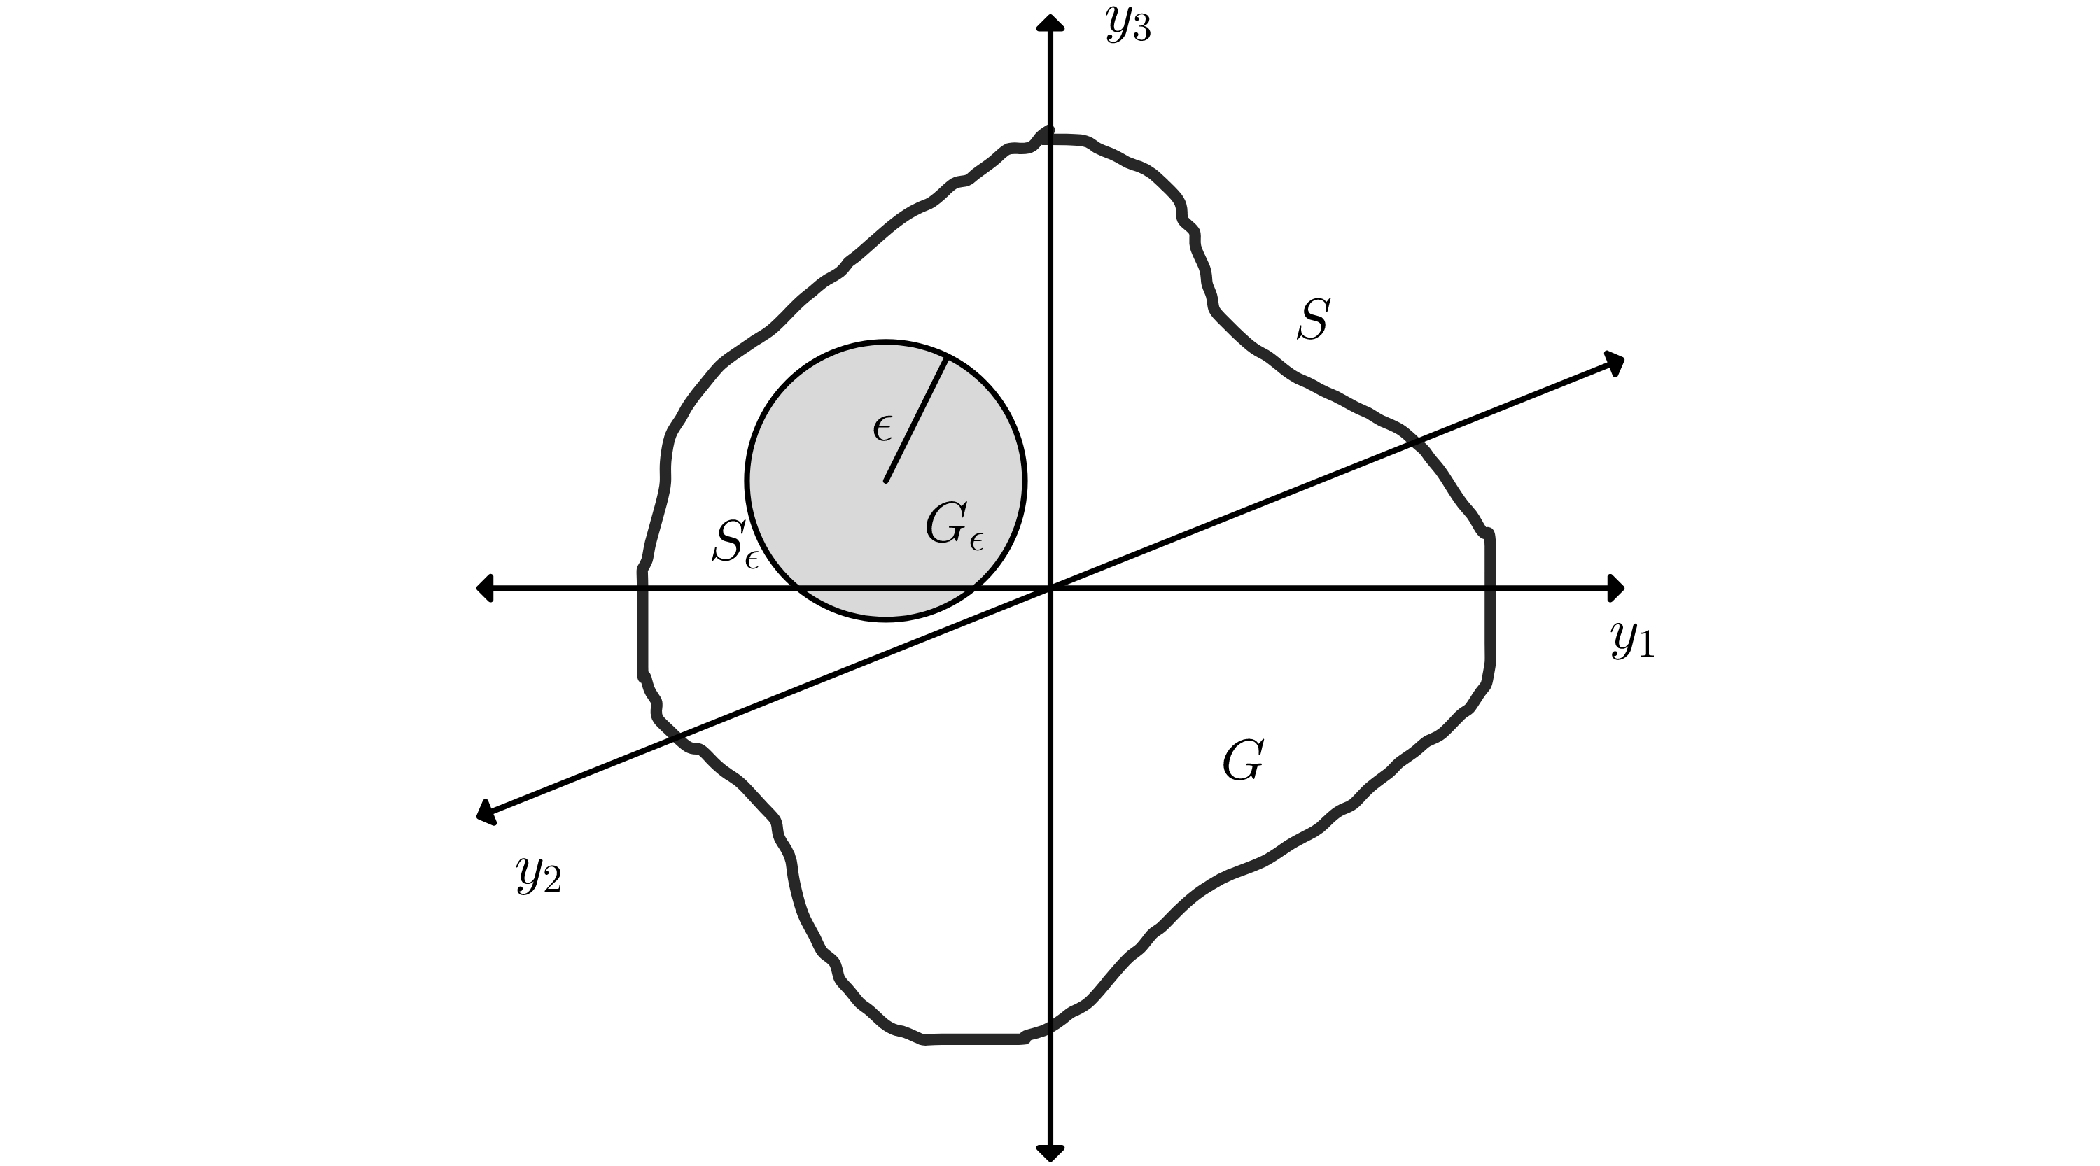
\includegraphics[scale=0.15]{rep.png}
\captionlabelfalse
\caption{The domain}
\end{center}
\end{figure}
\par
The domain $G$ is any continuous closed volume, with surface $S$, the domain $G_\epsilon$ is a sphere inside our volume, i.e. $G_\epsilon \in G$, with its center $x = (x_1,x_2,x_3)$, radius $\epsilon$, and surface $S_\epsilon$.    
\begin{align}
\nabla_{y}^{2} u(y) =0
\end{align}
Where
\begin{align}
u(y) \in C^3(G) \quad,\quad u(y) \in C^2(G\cup S)
\end{align}
From (2) the condition for using Green's identity between the pair of function $u$ and the potential function $E$ is satisfied since they are both continuous on our domain. 
\\
Thus using the identity yields.
\[
    \int_G \left[E(x,y)\nabla_{y}^{2} u(y) - u(y)\nabla_{y}^{2} E(x,y)\right]dx = \int_\Gamma \left[E(x,y)\frac{\partial u(y)}{\partial \vec{n}}-u(y)\frac{\partial E(x,y)}{\partial \vec{n}}\right] d\sigma    
\]
\[
  \because \nabla_{y}^{2} E(x,y) = 0  \quad,\quad  \nabla_{y}^{2} u(y) =0
\]
\[
    \int_\Gamma \left[E(x,y)\frac{\partial u(y)}{\partial \vec{n}}-u(y)\frac{\partial E(x,y)}{\partial \vec{n}}\right] d\sigma = 0    
\]
Since a sphere cutout was proposed then our region of study has two surfaces with the normal being opposite in direction thus the surface integral at hand can be split in two and we get.
\[
    \int_S \left[E(x,y)\frac{\partial u(y)}{\partial \vec{n}}-u(y)\frac{\partial E(x,y)}{\partial \vec{n}}\right] d\sigma - \int_{S_\epsilon} \left[E(x,y)\frac{\partial u(y)}{\partial \vec{n_\epsilon}}-u(y)\frac{\partial E(x,y)}{\partial \vec{n_\epsilon}}\right] d\sigma_\epsilon  = 0    
\]
The first term in the second integral vanishes due to spherical symmetry, 
\\and on $S_\epsilon$ we have $r=\epsilon$ then $E = \frac{1}{\epsilon}$ therefore $\displaystyle \frac{\partial E(x,y)}{\partial \vec{n_\epsilon}} = \frac{\partial}{\partial \epsilon}\frac{1}{\epsilon} = -\frac{1}{\epsilon^2}$
thus we are left with.
\[
    \int_S \left[E(x,y)\frac{\partial u(y)}{\partial \vec{n}}-u(y)\frac{\partial E(x,y)}{\partial \vec{n}}\right] d\sigma  = \frac{1}{\epsilon^2} \int_{S_\epsilon} u(y) d\sigma_\epsilon    
\]
By adding and subtracting $\displaystyle \frac{1}{\epsilon^2} \int_{S_\epsilon} u(x) d\sigma_\epsilon$ the following term from the right hand side.
\begin{align}
\int_S \left[E(x,y)\frac{\partial u(y)}{\partial \vec{n}}-u(y)\frac{\partial E(x,y)}{\partial \vec{n}}\right] d\sigma  &= \frac{1}{\epsilon^2} \left[\int_{S_\epsilon} (u(y) - u(x)) d\sigma_\epsilon + \int_{S_\epsilon} u(x) d\sigma_\epsilon\right]
\end{align}
We now show that the first integral on the right hand side vanishes as $\epsilon \to 0$.
\[
    \left|\int_{S_\epsilon} u(y)-u(x) d\sigma_\epsilon \right| \leq \int_{S_\epsilon} |u(y)-u(x)| d\sigma_\epsilon \leq \delta(\epsilon)\int_{S_\epsilon} d\sigma_\epsilon \leq 4\pi \delta(\epsilon)    
\]
As $\epsilon \to 0$ , $\delta(\epsilon) \to 0$
\\
Because the absolute value of the integral is $\leq$ 0 then it's equal 0. Now we evaluate the second integral.
\[
    \int_{S_\epsilon} u(x)d\sigma_\epsilon = u(x)\int_{S_\epsilon}d\sigma_\epsilon = u(x) 4\pi\epsilon^2
\]
Substituting in (3) we finally get the representation formula
\[
    u(x) = \frac{1}{4\pi} \int_S \left[E(x,y)\frac{\partial u(y)}{\partial \vec{n}}-u(y)\frac{\partial E(x,y)}{\partial \vec{n}}\right] d\sigma    
\]
\newpage
\setcounter{equation}{0}
\subsection{Laplace's Equation in Cylindrical Coordinates}
Considering the Dirichlet problem.
\[
    \begin{cases}
        \displaystyle \nabla^2 u(r,z) &= \frac{\partial^2 u(r,z)}{\partial z^2} + \frac{1}{r}\frac{\partial}{\partial r}\left[r\frac{\partial u(r,z)}{\partial r}\right] = 0 \;\; , \quad r >0
        \\
        \text{I.C} \quad &\Longrightarrow \quad u(r,0) = f(r)
        \\
        \text{B.C} \quad &\Longrightarrow \quad \lim_{r\rightarrow\infty} u(r,z) =0
    \end{cases}
\]
\begin{enrichment*}{Hanckel Transform}
    Let $f$ be a function in $r$ on the interval $[0,\infty]$, then the Hanckel transform is defined as.
    \[
        \hat{f}(\rho) = \int_{0}^{\infty} r J_o(r\rho) f(r) dr    
    \]
    Where $J_o$ is the Bessel function 
    \[
        J_o(z) = \frac{1}{2\pi}\int_{0}^{\infty} \cos(zcos\theta)d\theta     
    \]
    Which has the property 
    \[
        z J_o''(z) + J_o'(z)+ zJ_o(z) = 0     
    \]
    And the inverse Hanckel Transform is 
    \[
        f(r) = \int_{0}^{\infty} \rho J_o(r\rho) \hat{f}(\rho) d\rho    
    \]
\end{enrichment*}
By taking Hankel transformation for both sides
\begin{align*}
\frac{\partial^2 }{\partial z^2}\int_{0}^{\infty} rJ_o(r\rho)u(r,z) dr &+ \int_{0}^{\infty}rJ_o(r\rho)\frac{1}{r}\frac{\partial}{\partial r}\left[r\frac{\partial u(r,z)}{\partial r}\right]dr = 0
\\
\frac{\partial^2 \hat{u}(\rho,z)}{\partial z^2} &+ \int_{0}^{\infty}J_o(r\rho)\frac{\partial}{\partial r}\left[r\frac{\partial u(r,z)}{\partial r}\right]dr = 0
\\
\frac{\partial^2 \hat{u}(\rho,z)}{\partial z^2}  &= -\int_{0}^{\infty}J_o(r\rho)\frac{\partial}{\partial r}\left[r\frac{\partial u(r,z)}{\partial r}\right]dr    
\end{align*}
Now we write the right hand side as.
\begin{align*}
-\int_{0}^{\infty}J_o(r\rho)\frac{\partial}{\partial r}\left[r\frac{\partial u(r,z)}{\partial r}\right]dr &= -\int_{0}^{\infty}\frac{\partial}{\partial r}\left[J_o(r\rho)r\frac{\partial u(r,z)}{\partial r}\right]dr + \int_{0}^{\infty} r\frac{\partial u(r,z)}{\partial r} \rho J_o'(r\rho)dr
\\
&= -\left[rJ_o(r\rho)\frac{u(r,z)}{\partial r}\right]_{0}^{\infty} + \int_{0}^{\infty} r\rho\frac{\partial u(r,z)}{\partial r} J_o'(r\rho)dr
\\
&= \int_{0}^{\infty} r\rho\frac{\partial u(r,z)}{\partial r} J_o'(r\rho)dr
\end{align*}
The first term vanishes since Bessel functions tend to zero when $r$ approaches infinity
\begin{align*}
\int_{0}^{\infty} r\rho\frac{\partial u(r,z)}{\partial r} J_o'(r\rho)dr
&= \int_{0}^{\infty} \frac{\partial}{\partial r}\left[ r\rho\frac{\partial u(r,z)}{\partial r} J_o'(r\rho)\right]dr 
- \int_{0}^{\infty} \left[\rho J_o'(r\rho)+ r\rho^2 J_o''(r\rho)\right] u(r,z)dr
\\
&= \left[ r\rho\frac{\partial u(r,z)}{\partial r} J_o'(r\rho)\right]_{0}^{\infty} - \int_{0}^{\infty} \frac{1}{r}\left[r\rho J_o'(r\rho)+ r^2\rho^2 J_o''(r\rho)\right] u(r,z)dr
\\
&= - \int_{0}^{\infty} \frac{1}{r}\left[r\rho J_o'(r\rho)+ r^2\rho^2 J_o''(r\rho)\right] u(r,z)dr
\end{align*}
From the bassel function property we get.
\begin{align*}
- \int_{0}^{\infty} \frac{1}{r}\left[r\rho J_o'(r\rho)+ r^2\rho^2 J_o''(r\rho)\right] u(r,z)dr &= \int_{0}^{\infty} \frac{1}{r}\left[r^2\rho^2 J_o(r\rho)\right] u(r,z)dr
\\
&= \rho^2 \int_{0}^{\infty} r J_o(r\rho) u(r,z)dr = \rho^2 \hat{u}(\rho,z)
\end{align*}
Therefore we can get.
\[
    \frac{\partial^2 \hat{u}(\rho,z)}{\partial z^2} = \rho^2 \hat{u}(\rho,z)    
\]
Which have the solution. 
\[
\hat{u}(\rho,z) = A e^{\rho z} + Be^{-\rho z}    
\]
And from the boundary condition after taking the Hankel transformation for it $\hat{u}(\rho,z)$ is convergent as $\rho \to \infty$
\[
\therefore A = 0    
\]
And preforming the Hankel transform on the initial condition.
\[
\hat{u}(\rho,0) = B = \hat{f}(\rho)    
\]
\[
\hat{u}(\rho,z) = \hat{f}(\rho)e^{-\rho z}    
\]
Now to find $u$ we preform the inverse Hankel Transform.
\[
u(r,z) = \int_{0}^{\infty} \rho J_o(r\rho)\hat{f}(\rho)e^{-\rho z} d\rho    
\]

\newpage
\setcounter{equation}{0}
\section{Burger's Equation}
Burger's equation  is a partial differential equation occurring in various areas of applied mathematics. 
It has many forms, we will be studying the solution of one of its forms
the viscous Burger's equation Cauchy problem, occurring in fluid dynamics, 
the viscous equation is non linear thus needs a different approach than those used earlier. 
We will be using the method of Hopf-Cole.
\begin{equation}
    \begin{cases}
        \displaystyle \frac{\partial u(x,t)}{\partial t} + u(x,t)\frac{\partial u(x,t)}{\partial x} = \gamma \frac{\partial^2 u(x,t)}{\partial x^2} \tquad \gamma > 0 , x \in \mathbb{R}
        \\
        \text{I.C} \quad \Longrightarrow \quad u(x,0) = f(x)
    \end{cases}
\end{equation}
\begin{enrichment*}{}
    if $\gamma = 0$ the equation is called the in-viscous Burger's equation
\end{enrichment*}
We start our treatment by defining a new function
\[
v(x,t) = e^{\alpha\phi(x,t)}  \quad \Longrightarrow \quad \phi(x,t) = \frac{1}{\alpha}\ln(v(x,t))
\]
We try to find the function $\phi$ such that $v$ satisfy
\begin{equation}
    \begin{cases}
        \displaystyle \frac{\partial v}{\partial t} = \gamma \frac{\partial^2 v}{\partial x^2}
        \\
        \text{I.C} \quad \Longrightarrow \quad v(x,0) = g(x)
    \end{cases}
\end{equation}
We start finding the terms of the equation (2) in terms of $\phi$
\begin{align*}
\hspace{2cm}
\frac{\partial v}{\partial t} &= \alpha e^{\alpha\phi} \frac{\partial \phi}{\partial t}
\\
\frac{\partial v}{\partial x} &= \alpha e^{\alpha\phi} \frac{\partial \phi}{\partial x} 
\\
\frac{\partial^2 v}{\partial x^2} &= \alpha^2 e^{\alpha \phi} {\left(\frac{\partial \phi}{\partial x}\right)}^2 + \alpha e^{\alpha\phi} \frac{\partial^2 \phi}{\partial x^2}
\end{align*}
Substitute in (2)
\begin{align}
\alpha e^{\alpha\phi} \frac{\partial \phi}{\partial t} &= \gamma\left(\alpha^2 e^{\alpha \phi} {\left(\frac{\partial \phi}{\partial x}\right)}^2 + \alpha e^{\alpha\phi} \frac{\partial^2 \phi}{\partial x^2}\right)\nonumber
\\
\frac{\partial \phi}{\partial t} &= \gamma\alpha {\left(\frac{\partial \phi}{\partial x}\right)}^2 + \gamma \frac{\partial^2 \phi}{\partial x^2}
\end{align}
Differentiating with respect to $x$ and changing the order of differentiation on the left hand side
\[
    \frac{\partial }{\partial t}\left[ \frac{\partial \phi}{\partial x}\right] = 2\gamma\alpha \frac{\partial\phi}{\partial x}\frac{\partial^2 \phi }{\partial x^2} + \gamma\frac{\partial^3 \phi}{\partial x^3}    
\]
Now put $\displaystyle u(x,t) = \frac{\partial \phi(x,t)}{\partial x}$
\[
    \frac{\partial u }{\partial t} = 2\gamma\alpha u\frac{\partial u}{\partial x} + \gamma\frac{\partial^2 u}{\partial x^2}    
\]
Set $2\gamma\alpha = -1$ we get
\[
    \frac{\partial u }{\partial t} + u\frac{\partial u}{\partial x} = \gamma\frac{\partial^2 u}{\partial x^2}    
\]
Means that $\displaystyle \frac{\partial \phi(x,t)}{\partial x}$ is a solution for the burger equation 
\\
We know that problem (2) is the heat equation Cauchy problem that we solved before using Poisson's formula and we know that the solution is 
\[
v(x,t) = \frac{1}{\sqrt{4\pi \gamma t}} \int_{-\infty}^{\infty} e^{\textstyle -\frac{(x-y)^2}{4\gamma t}} g(y)dy    
\]
Finding $v$ will get us $\phi$ from the relation $\displaystyle \phi(x,t) = \frac{1}{\alpha}\ln(v(x,t))$ then differentiating it with respect to $x$ to finally find $u$.

\section{Introduction To Integral Equations}
\
\begin{definition}[Integral equations]
    Are equations in which an unknown function appears under an integral sign.
\end{definition}
There is a close connection between differential and integral equations, 
there are some differential equations problems can be transform to integral equations and the other way around.

\subsection{Successive Approximation}
\
\begin{definition}[Successive Approximation Method]
    Is a numerical technique used to solve equations or find the roots of functions that cannot be solved analytically. It is an iterative process in which you start with an initial guess for the solution and then repeatedly refine that guess to get closer and closer to the actual solution.
\end{definition}

In the context of integral equations, the successive approximation method is a powerful technique for solving integral equations of the form:
\[
\phi(x) = f(x) + \lambda\int_{a}^{b} K(x,t) \phi(t)dt    
\]
Where $\phi(x)$ is the unknown function to be determined,
$f(x)$  is a given function, $K(x,y)$ is the kernel of the integral equation,
And $\lambda$ is a constant parameter.

The successive approximation method is an iterative approach that allows us to find an approximate solution to this integral equation by breaking it down into simpler steps. Here's how it works:

\begin{enumerate}[itemsep=10pt]
    \item \textbf{Choose an Initial Guess}: Start with an initial guess $\phi_0(x)$ for the unknown function $\phi(x)$. This guess can be any reasonable function that satisfies any known boundary or initial conditions most of the time it's chosen to be 0 or $f(x)$.
    \item \textbf{Update the Guess}: Substitute the initial guess for $\phi(x)$ into the integral equation and calculate an updated function $\phi_1(x)$ :
    \[
       \phi_1(x) = f(x) + \lambda\int_{a}^{b} K(x,t) \phi_0(t)dt     
    \]
    \item \textbf{Check for Convergence}: Check the difference between the updated function $\phi_1(x)$ and the previous approximation. If the difference is below a certain tolerance level or satisfies a convergence criterion, stop the iterations and consider $\phi_1(x)$ as the final approximation. Otherwise, continue to the next step.
    \item \textbf{Repeat the Process}: Use $\phi_1(x)$ as the new approximation and repeat the process. Substitute $\phi_1(x)$ into the integral equation to find a new approximation $\phi_2(x)$ , and so on. Continue iterating until the solution converges to the desired accuracy.
    \item \textbf{Termination Criteria}: Decide on a termination condition to stop the iterations, similar to the termination criteria in the general successive approximation method. This could be based on a maximum number of iterations or reaching a desired level of accuracy.    
    \item \textbf{Final Result}: Once the termination condition is met, the last obtained approximation $\phi_n(x)$ is considered the solution to the integral equation.
\end{enumerate}
It's important to note that the convergence of the successive approximation method for integral equations 
may not always be guaranteed
depends on various factors, including the nature of the kernel $K(x,y)$, the choice of the initial guess, 
and the value of the parameter 

$\lambda$. In some cases, convergence may be slow or may not occur at all. In such situations, other numerical methods tailored for specific types of integral equations may be more appropriate.


\subsection{Fredholm's Integral Equation}
Consider the following integral equation.
\[
u(x) = f(x) + \lambda\int_{a}^{b} K(x,y) u(y)dy    
\]
Where $f(x)$ and $K(x,y)$ are given continuous function on $[a,b]\times[c,d]$ and
\[
    G := \left\{ (x,y) | \quad a\leq x\leq b \quad \text{and} \quad c\leq y\leq d \right\}
\]
We try to determine the function $u(x)$ using the successive approximation method.
\begin{align*}
u_1(x) &= f(x) + \lambda\int_{a}^{b} K(x,y) u_o(y)dy
\\
u_2(x) &= f(x) + \lambda\int_{a}^{b} K(x,y) u_1(y)dy
\\
\vdots
\\
u_{n+1}(x) &= f(x) + \lambda\int_{a}^{b} K(x,y) u_n(y)dy
\end{align*}
Let us choose.
\[
u_o(x) = f(x)    
\]
Then.
\begin{align*}
u_1(x) &= u_o(x) + \lambda\int_{a}^{b} K(x,y) u_o(y)dy
\\
u_1(x)- u_o(x) &= \lambda\int_{a}^{b} K(x,y) u_o(y)dy
\end{align*}
Since the integral is finite and the functions are continuous on the limits of integration 
this can be considered as the inner product of the two functions 
that will be less than or equal to their magnitudes where $|K(x,y)| = M$ and $|f(x)| = m$.
\begin{enrichment*}{}
    The inner product of two functions on the space of continuous functions is defined as 
    \[
        <f,g> = \int f(x)g(x)dx \leq |f(x)||g(x)|
    \]
    Remember the inner product of vectors $\vec{v}\cdot \vec{u} = vu \cos(\theta) \leq vu$
\end{enrichment*}
\begin{align*}
    \left|u_1(x)- u_o(x)\right| &= |\lambda|\left|\int_{a}^{b} K(x,y) u_o(y)dy\right|    
    \\
    & \leq |\lambda|\int_{a}^{b}|K(x,y)||u_o(y)|dy = |\lambda|Mm\int_{a}^{b}dy
    \\
    & \leq |\lambda|Mm(b-a)
\end{align*}
We also have in the same manner. 
\begin{align*}
u_2(x) &= f(x) + \lambda\int_{a}^{b} K(x,y) u_1(y)dy
\\
u_2(x) - u_1(x)&= \lambda\int_{a}^{b} K(x,y) [u_1(y)-u_o(y)]dy
\\
|u_2(x) - u_1(x)| &= |\lambda|\left|\int_{a}^{b} K(x,y) [u_1(y)-u_o(y)]dy\right| 
\\
&\leq |\lambda|M |\lambda|Mm(b-a) \int_{a}^{b}dy = |\lambda|^2M^2{(b-a)}^2 m
\end{align*}
And by induction we can find.
\[
    |u_{k}(x) - u_{k-1}(x)| \leq |\lambda|^kM^k {(b-a)}^k m    
\]
We note that.
\begin{align*}
u_o(x) + \sum_{k=1}^{n} [u_{k}(x) - u_{k-1}(x)] &= u_o + u_1 - u_o + u_2 - u_1 + u_3 - u_2 + ...+u_n - u_{n-1}
\\
&= u_n(x)
\end{align*}
We can find the solution $u(x)$ by taking the limit to $\infty$
\[
    \lim_{n\to\infty} u_n(x) = u(x) = u_o(x) + \sum_{k=1}^{\infty} [u_{k}(x) - u_{k-1}(x)] \leq u_o(x) + m\sum_{k=1}^{\infty} {(|\lambda|M(b-a))}^k    
\]
This is geometric series if $|\lambda|M(b-a) < 1$ then the series converges absolutely and uniformally
\begin{example}
    Consider the Fredholm integral equation 
    \[
        u(x) = e^x + e^{-1}\int_{0}^{1}u(y)dy    
    \]
    We can select any real value function for the initial guess then we set 
    \[
    u_0(x) =f(x) =e^x 
    \]
    Now to get $u_1(x)$
    \[
        u_1(x) = e^x + e^{-1}\int_{0}^{1}e^y dy        
    \]
    And that gives us the first approximation of $u(x)$ by
    \[
        u_1(x) = e^x + 1 - e^{-1} 
    \]
    Now to get $u_2(x)$
    \[
        u_2(x) = e^x + e^{-1}\int_{0}^{1}e^y + 1 - e^{-1}dy = e^x + 1 - e^{-2}
    \]
    This gives us the second approximation of $u(x)$
    \\
    Continue in the same manner we find the third approximation of $u(x)$
    \[
        u_3(x) = e^x + 1 - e^{-3}
    \]
    Proceeding as before we can obtain the $n^{\text{th}}$ approximation
    \[
        u_n(x) = e^x + 1 - e^{-n} , \quad n \geq 1
    \]
    Now to get the solution taking the limit as $n \to \infty$
    \begin{align*}
        u(x) &= \lim_{n\to\infty} u_n(x)
        \\
        &= \lim_{n\to\infty} e^x + 1 - e^{-n}
        \\
        &= e^x + 1
    \end{align*}
\end{example}
\begin{example}
    Consider the Fredholm integral equation 
    \[
        u(x) = x + \lambda\int_{0}^{1} xt u(t)dt
    \]
    For the zeroth approximation we set 
    \[
    u_0(x) = x
    \]
    Then we get get $u_1(x)$
    \[
        u_1(x) = x + \lambda\int_{0}^{1} xt^2dt
    \]
    And that gives us the first approximation of $u(x)$ by
    \[
        u_1(x) = x + \frac{\lambda}{3}x
    \]
    Now to get $u_2(x)$
    \[
        u_2(x) = x + \lambda\int_{0}^{1} xt\left(t + \frac{\lambda}{3}t\right)dt = x +\frac{\lambda}{3} x +\frac{\lambda^2}{9} x
    \]
    This gives us the second approximation of $u(x)$
    \\
    Proceeding as before we can obtain the $n^{\text{th}}$ approximation
    \[
        u_n(x) = x +\frac{\lambda}{3} x +\frac{\lambda^2}{9} x + \dots + \frac{\lambda^{n-1}}{3^{n-1}} x , \quad n \geq 1
    \]
    \[
        u_n(x) = x\sum_{k=0}^{n} {\left(\frac{\lambda}{3}\right)}^{k}
    \]
    Now to get the solution taking the limit as $n \to \infty$
    \begin{align*}
        u(x) &= \lim_{n\to\infty} u_n(x)
        \\
        &= x\sum_{k=0}^{\infty} {\left(\frac{\lambda}{3}\right)}^{k}
    \end{align*}
    This is geometric series if $|\lambda| < 3$ and $\lambda \neq 0$ it's value will be 
    \[
    u(x) = \frac{3}{3-\lambda}x, \quad  |\lambda| < 3,\lambda \neq 0
    \]
\end{example}
\subsection{Volttera Integral Equation}
Volterra integral equations have wide applications in areas like control theory, 
population dynamics, signal processing, and modeling dynamic systems. 
There are different forms of it, such as Volterra integral equations of the second kind, exist to address specific scenarios and applications.
\par 
Consider the following  integral equation.
\[
u(x) = f(x) + \int_{0}^{x} K(x,y) u(y)dy
\]
Where the functions $f(x)$ is a given function, often called the "forcing function" or "input function."
and $K(x,y)$ is a given kernel function
\\
To solve this equation we use, as we did with Fredholm's integral equation, the method f successive approximation. We first define a sequence.
\[
u_n(x) = f(x) + \int_{0}^{x} K(x,y) u_{n-1}(y)dy    
\]
We can choose our first term arbitrary but here we choose it to be $u_0(x) = f(x)$ then we getting.
\begin{align*}
u_1(x) &= u_0(x) + \int_{0}^{x} K(x,y) u_0(y)dy
\\
u_1(x) - u_0(x) &= \int_{0}^{x} K(x,y) f(y)dy
\end{align*}
From this as before we can see that.
\[
|u_1(x) - u_0(x)| \leq mMx
\]
\[
\because M=\sup|K(x,y)| \quad , \quad m=\sup |f(x)|        
\]
Then we continue in the same way.
\begin{align*}
u_2(x) - u_1(x) &= \int_{0}^{x} k(x,y) [u_1(x) - u_0(x)] dy
\\
|u_2(x) - u_1(x)| &\leq mM^2\frac{x^2}{2}
\end{align*}
And by induction we find that.
\[
|u_n(x) - u_{n-1}(x)| \leq mM^n\frac{x^n}{n!}    
\]
Now we study the series.
\begin{align*}
u_0 + \sum_{k=1}^{n} [u_k-u_{k-1}] &= u_0 + u_1 - u_0 +u_2 - u_1 + \cdots +u_{n-1}-u_{n-2}+ u_n - u_{n-1} 
\\
&= u_n
\end{align*}
Taking the limit as n approaches infinity
\begin{align*}
u(x) = \lim_{n\to \infty} u_n(x) &= u_0 + \sum_{k=1}^{\infty} [u_k-u_{k-1}]    
\\
& \leq m\sum_{k=1}^{\infty} \frac{{(xM)}^k}{k!} = m e^{xM}
\end{align*}
And we can deduce that the sum is uniformally convergent and we can find $u(x)$ because the factorial is more powerful that the exponential.

\newpage
\subsection{Abel Integral Equation}
Abel integral equation belongs to the class of Volterra equations of the first kind
it's expressed in the following general form:
\[
f(x) = \int_{0}^{x} \frac{\phi(\tau)}{{(x-\tau )}^\alpha} d\tau
\]
Where $0<\alpha<1$ is known constants, $f(x)$ is a known function and $\phi(\tau)$ is unknown function,
The expression ${(x-\tau )}^\alpha$  is called the kernel of the Abel integral equation, or Abel kernel
\\
Now by multiplying both sides with $\displaystyle \frac{1}{{(t-x)}^{1-\alpha}}$
\[
\frac{f(x)}{{(t-x)}^{1-\alpha}} = \frac{1}{{(t-x)}^{1-\alpha}} \int_{0}^{x} \frac{\phi(\tau)}{{(x-\tau)}^\alpha} d\tau
\]
And integrating with respect to $x$ from $0 \to t$
\[
\int_{0}^{t} \frac{f(x)}{{(t-x)}^{1-\alpha}} dx=  \int_{0}^{t} \frac{1}{{(t-x)}^{1-\alpha}} \int_{0}^{x} \frac{\phi(\tau)}{{(x-\tau)}^\alpha} d\tau dx
\]
By switching the order of the integration 

\begin{center}
        \begin{tikzpicture}
            \draw[->] (0,0,0) -- (3,0,0) node[right]{$x$};
            \draw[->] (0,0,0) -- (0,3,0) node[above]{$\tau$};
            \draw[->, blue] (0,0,0) -- (2.5,2.5,0) node[above right]{$\tau = x $};
            \draw[->, orange] (0,2.2,0) -- (2.7,2.2,0) node[right]{$\tau = t$};
		
            \draw[-,red] (0,1,0)--(1,1,0);
            \draw[-,red] (0,1.2,0)--(1.2,1.2,0);

            \fill [oblique lines] (0,1,0) -- (1,1,0) -- (1.2,1.2,0) -- (0,1.2,0);
            \fill [oblique lines] (1,1,0) -- (1,2.2,0) -- (1.2,2.2,0) -- (1.2,1.2,0);

            \draw[-,red] (1,1,0)--(1,2.2,0);
            \draw[-,red] (1.2,1.2,0)--(1.2,2.2,0);

            \draw (-.2,1.1,0) node{$d\tau$};
            \draw (1.1,2.4,0) node{$dx$};
	\end{tikzpicture}
\end{center}
\[
\int_{0}^{t} \frac{f(x)}{{(t-x)}^{1-\alpha}} dx= \int_{0}^{t}\int_{\tau}^{t} \frac{1}{{(t-x)}^{1-\alpha}{(x-\tau)}^\alpha} dx \phi(\tau) d\tau
\]
Taking the inner integral and put $x = \tau + (t-\tau)\xi \Longrightarrow dx = (t-\tau)d\xi$
\begin{align*}
    \int_{0}^{1} \frac{(t-\tau)}{{(t-\tau)}^\alpha \xi^{\alpha} {(t-\tau-(t-\tau)\xi)}^{1-\alpha}} d\xi 
    &= \int_{0}^{1} \frac{(t-\tau)}{{(t-\tau)}^\alpha \xi^\alpha {(t-\tau)}^{-\alpha}{(1-\xi)}^{1-\alpha}} d\xi
    \\
    &= \int_{0}^{1} \frac{1}{\xi^{\alpha} {(1-\xi)}^{1-\alpha} } d\xi
\end{align*}
this is the form of the $\beta$ function
\begin{align*}
    \int_{0}^{1} \frac{1}{\xi^{\alpha} {(1-\xi)}^{1-\alpha} } d\xi &= \int_{0}^{1} \xi^{-\alpha} {(1-\xi)}^{\alpha-1} d\xi
    \\
    &=\beta (1-\alpha,\alpha) = \frac{\pi}{\sin(\alpha\pi)}
\end{align*}
Then
\[
\int_{0}^{t} \frac{f(x)}{{(t-x)}^{1-\alpha}} dx = \int_{0}^{t} \frac{\pi}{\sin(\alpha\pi)} \phi(\tau) d\tau
\]
Taking the derivative for $t$ 
\[
\frac{d}{dt} \int_{0}^{t} \frac{f(x)}{{(t-x)}^{1-\alpha}} dx = \frac{\pi}{\sin(\alpha\pi)} \phi(t)
\]
Therefore $\phi(t)$ can be written as 
\[
\phi(t) = \frac{\sin(\alpha\pi)}{\pi}  \frac{d}{dt} \int_{0}^{t} \frac{f(x)}{{(t-x)}^{1-\alpha}} dx
\]
This is the solution of Abel Integral equation

\newpage

\section{Energy Integral}
\
\begin{definition} [The Energy Integral]
    Is a mathematical expression that represents the total energy of a vibrating string.
\end{definition}
$E(t)$ in one dimension is defined as :
\[
E(t)  =  \frac{\rho}{2} \int {\left(\frac{\partial u}{\partial t}\right)}^2 dx + \frac{\mu}{2} \int {\left(\frac{\partial u}{\partial x}\right)}^2 dx
\] 
\begin{itemize}
    \item $\rho$ is the constant density
    \item $\mu$ is the coefficient of tension of the string
    \item $\displaystyle \frac{\rho}{2} \int {\left(\frac{\partial u}{\partial t}\right)}^2 dx $ corresponds to the "kinetic energy" of the body (in analogy with $\frac{1}{2}mv^2$, the kinetic energy of a particle of mass m and velocity v)
    \item $\displaystyle \frac{\mu}{2} \int {\left(\frac{\partial u}{\partial x}\right)}^2 dx $ corresponds to the "potential energy".
\end{itemize}

The energy integral is essential because it helps us understand how energy is distributed in the wave as it propagates through space and time. It also plays a crucial role in analyzing the behavior of waves, their interactions with other waves or boundaries, and studying the overall dynamics of wave phenomena in various physical systems.

\subsection{Energy Conservation For 1D Wave Equation}
To prove that the energy integral is conservative over the wave equation in 1D,
we need to show that the total energy of the system remains constant over time, i.e., the derivative of the energy with respect to time is zero.
\par
Let's consider the wave equation
\[
    \frac{\partial^2 u(x,t)}{\partial t^2} = c^2 \frac{\partial^2 u(x,t)}{\partial x^2} \dquad c^2 = \frac{\mu}{\rho} \dquad x \in [a,b] \text{ (string length)}
\]
\vspace*{-.2cm}
\begin{theorem}
    Let $g : \mathbb{R}\times\mathbb{R} \to \mathbb{R}$ be a continuous function such that $\displaystyle \frac{\partial g(x,t)}{\partial t}$ exist and is continuous.
    \\
    Suppose $\displaystyle \int_{-\infty}^{\infty} |g(x,t)| dx $  and   $\displaystyle \int_{-\infty}^{\infty} |\frac{\partial g(x,t)}{\partial t}| dx $ exists for each $t$
    and that $\displaystyle \int_{|x|>R} |\frac{\partial g(x,t)}{\partial t}| dx \to 0 $ as $R \to \infty$ uniformly in $t$ on every interval $[a,b]$.\
    \\
    Then $\displaystyle \int_{-\infty}^{\infty} g(x,t) dx $ is differentiable with :
    \[
        \frac{\partial}{\partial t} \int_{-\infty}^{\infty} g(x,t) dx = \int_{-\infty}^{\infty} \frac{\partial g(x,t)}{\partial t} dx
    \]
\end{theorem}
By differentiate $E(t)$ and let's say for now that 
$\displaystyle {\left(\frac{\partial u}{\partial t}\right)}^2$
And
$\displaystyle {\left(\frac{\partial u}{\partial x}\right)}^2$
satisfies theorem 8.1 it will be explained later 
\[
E'(t) = \frac{\rho}{2} \int_{a}^{b} 2\frac{\partial u}{\partial t}\frac{\partial^2 u}{\partial t^2} dx + \frac{\mu}{2} \int_{a}^{b} 2\frac{\partial u}{\partial x}\frac{\partial^2 u}{\partial t\partial x} dx    
\]
By integrating by parts for the second integral 
\[
E'(t) = \rho \int_{a}^{b} \frac{\partial u}{\partial t}\frac{\partial^2 u}{\partial t^2} dx +\mu\left[\frac{\partial u}{\partial x}\frac{\partial u}{\partial t}\right]_{a}^{b} -\mu \int_{a}^{b} \frac{\partial u}{\partial t}\frac{\partial^2 u}{\partial x^2} dx    
\]
Assuming that initial conditions on the derivatives are
$\displaystyle \frac{\partial u(a,t)}{\partial t} = \frac{\partial u(b,t)}{\partial t} = 0$
In other words the ends are fixed so there is no movement and hence no velocity
\[
\therefore E'(t) = \rho \int_{a}^{b} \frac{\partial u}{\partial t}\frac{\partial^2 u}{\partial t^2} dx -\mu \int_{a}^{b} \frac{\partial u}{\partial t}\frac{\partial^2 u}{\partial x^2} dx    
\]
From the wave equation we get 
\begin{align*}
    E'(t) &= \rho c^2 \int_{a}^{b} \frac{\partial u}{\partial t}\frac{\partial^2 u}{\partial x^2} dx -\mu \int_{a}^{b} \frac{\partial u}{\partial t}\frac{\partial^2 u}{\partial x^2} dx    
    \\
    &= \mu \int_{a}^{b} \frac{\partial u}{\partial t}\frac{\partial^2 u}{\partial x^2} dx -\mu \int_{a}^{b} \frac{\partial u}{\partial t}\frac{\partial^2 u}{\partial x^2} dx = 0
\end{align*}
That shows us that $E(t)$ is constant for all $t$
\par
In a more general context by starting with the kinetic energy
\[
K.E = \frac{\rho}{2} \int_{-\infty}^{\infty} {\left(\frac{\partial u}{\partial t}\right)}^2 dx    
\]
To get convergence of the integral we have to assume that the integrand vanishes
outside of some large interval $|x| \leq R$.
To see whether the K.E is conserved in time
we differentiate with respect to time and we get
\[
\frac{d}{dt}K.E = \frac{\rho}{2} \int_{-\infty}^{\infty} 2\frac{\partial u}{\partial t}\frac{\partial^2 u}{\partial t^2} dx = \mu \int_{-\infty}^{\infty} \frac{\partial u}{\partial t}\frac{\partial^2 u}{\partial x^2} dx
\]
The final integral does not look like it would be zero but if we integrate by
parts we come up with something useful:
\[
    \mu \int_{-\infty}^{\infty} \frac{\partial u}{\partial t}\frac{\partial^2 u}{\partial x^2} dx = \mu \left[\frac{\partial u}{\partial t}\frac{\partial u}{\partial x}\right]_{-\infty}^{\infty} - \mu \int_{-\infty}^{\infty} \frac{\partial u}{\partial x}\frac{\partial^2 u}{\partial x \partial t} dx
\]
Now $\displaystyle \left[\frac{\partial u}{\partial t}\frac{\partial u}{\partial x}\right]_{-\infty}^{\infty} $ should vanish because the derivatives ought to approach zero in the limit. So we are left with:
\[
\frac{d}{dt}K.E = -\frac{d}{dt}\left(\frac{\mu}{2} \int_{-\infty}^{\infty} {\left(\frac{\partial u}{\partial t}\right)}^2 dx\right)
\]
And because the potential Energy is defined as 
\[
P.E = \frac{\mu}{2} \int_{-\infty}^{\infty} {\left(\frac{\partial u}{\partial t}\right)}^2 dx
\]
Then 
\[
   \frac{d}{dt}K.E = \frac{d}{dt}P.E 
\]
Or 
\[
\frac{d}{dt} \left(K.E + P.E \right) = 0    
\]
Then that says that the total energy $E(t)$ is conservative
\subsubsection*{Differentiating Under Integral}
As can be seen from the Theorem, we need continuity of 
$\displaystyle \frac{\partial g(x, t)}{\partial t}$
Where $g(x,t)$ is 
$\displaystyle {\left(\frac{\partial u}{\partial t}\right)}^2$
And
$\displaystyle {\left(\frac{\partial u}{\partial x}\right)}^2$. 
From physical considerations the energy is finite so that we should have existence of
$\displaystyle \int_{a}^{b} |g(x,t)|dx$. As for the integral
$\displaystyle \int_{-\infty}^{\infty} \left|\frac{\partial g(x,t)}{\partial x}\right|dx$
, it has to exist for each $t$. In our case there is a finite spatial interval of integration
[a, b] so that given the continuity of the derivatives on this interval there ought
to be no blow ups so we can assume this condition is satisfied for all t. 
The final condition in the theorem requires
$\displaystyle \int_{|x|>R} |\frac{\partial g(x,t)}{\partial t}| dx \to 0 $ as $R \to \infty$
and since we are dealing with a finite spatial interval this should also be satisfied.
Hence, differentiating under the integral sign is acceptable.

\subsection{Energy Conservation For 3D Wave Equation}
Let's consider the wave equation in 3d
\[
u_{tt} = \nabla_x^2 u \quad,\quad B.C \Longrightarrow  u(x,y)|_\Gamma = 0
\]
The Energy Integral will be as following
\[
    E = \iiint_{D}(u_t^2 + |\nabla_x u|^2) dx
\]
Suppose $u$ is smooth so that $u_{x_{i}t}=u_{t x_{i}}$, 
and the energy is bounded, then we can put the differentiation inside the integral sign:
\[
\frac{dE}{dt} = \iiint_{D}(  2 u_t u_{tt} + 2 \nabla_x u \cdot (\nabla_x u)_t) dx
\]
Now because $u_{tt} = \nabla_x^2 u$ then
\[
    \frac{dE}{dt} = \iiint_{D}(  2 u_t \nabla_x^2 u + 2 \nabla_x u \cdot (\nabla_x u)_t) dx
\]
Use Green's identities (integration by parts using divergence theorem):
\[
    \iiint_{D} \psi \nabla^2 \phi dx = -\iiint_{D} \nabla \psi \cdot \nabla \phi dx + \iint \psi (\nabla \phi \cdot n )dS
\]
Where $\psi = u_t $ and  $\phi = u$
\[
    \frac{dE}{dt} = \iiint_{D}( -2 \nabla_x u \cdot \nabla_x (u_t) + 2\nabla_x u \cdot (\nabla_x u)_t) dx  + \iint u_t(\nabla_x u \cdot n )d\Gamma
\]
From the boundary condition $u=0$ on $\Gamma$ then 
\[
    u_t(\nabla_x u \cdot n ) = 0
\]
\[
  \therefore  \frac{dE}{dt} = \iiint_{D}( -2 \nabla_x u \cdot \nabla_x (u_t) + 2\nabla_x u \cdot (\nabla_x u)_t) dx
\]
And because $u$ is smooth thus $\nabla_x (u_t) =(\nabla_x u)_t$
\[
  \therefore  \frac{dE}{dt} = \iiint_{D}( -2 \nabla_x u \cdot \nabla_x (u_t) + 2 \nabla_x u \cdot \nabla_x (u_t)) dx
\]
\[
    \therefore  \frac{dE}{dt} = 0
\]
Therefore the energy $E(t)$ is conservative on 3D wave equation and same method can be applied with 
$n^{\text{th}}$ dimension 